\documentclass[text01.tex]{subfiles}
\begin{document}
%
% section 1.2
%
\section{ラズベリーパイになれよう（１）}

%
% subsection 1.2.1
%
\subsection{ファイルとフォルダ}

コンピュータやラズベリーパイの中にあるデータ（音楽、動画、写真、テキストなど）はすべてファイルとして\ruby{扱}{あつか}われています。
ファイルには.(ドット)から始まる「\ruby{拡張子}{かくちょうし}」がついています。
拡張子は、どんな種類のファイルかを表します。
例えば\ruby{画像}{がぞう}ファイルには.jpgや.png、動画ファイルには.mp4、テキストファイルには.txt、ホームページには.htmlなどが使われます。

ファイルの他にフォルダがあります。フォルダはファイルをまとめて\ruby{保存}{ほぞん}するための入れ物のようなものです。
ファイルを書類とすると、フォルダはそれをまとめるバインダに例えることができます。
フォルダの中にフォルダを入れることもできます。

\begin{figure}[hb]
  \centering
    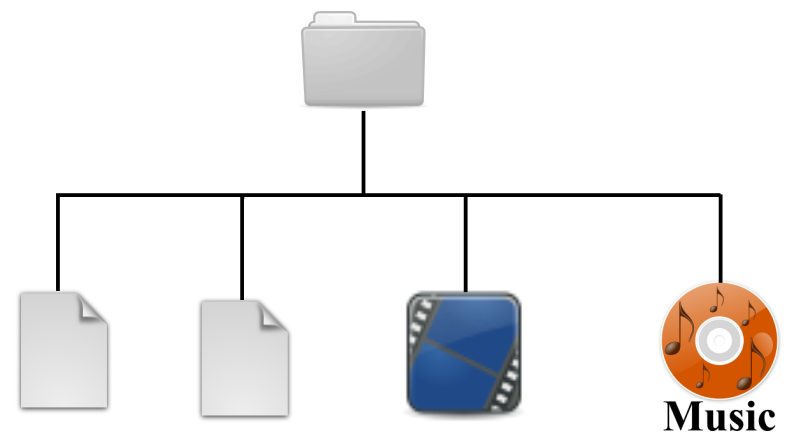
\includegraphics[keepaspectratio, height=50mm]{../../asset/image/figure15.png}
    \caption{フォルダとファイルの関係}
    \label{fig:19}
\end{figure}

% \begin{figure}[htbp]
%   \begin{minipage}[b]{0.32\linewidth}
%     \centering
%     \textbf{左 クリック}
%     \newline
%     カチッ
%     \newline
%     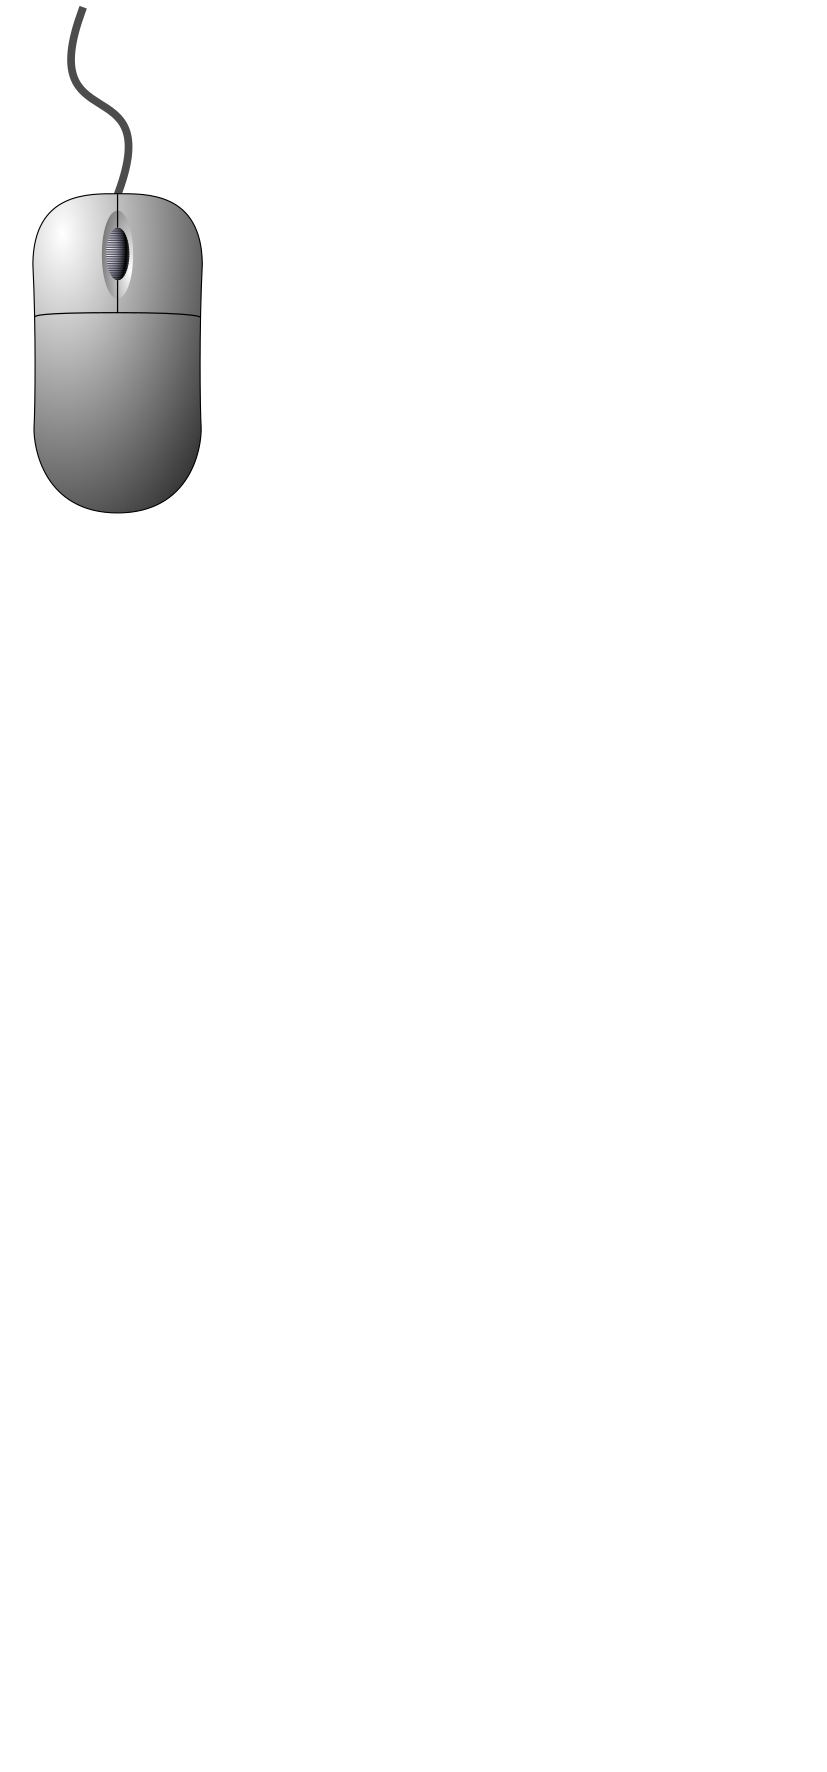
\includegraphics[keepaspectratio, height=30mm]{../../asset/image/textbook-img076.eps}
%     % \newline
%     % \small{1. ラズベリーパイ}
%     % \newline
%   \end{minipage}
%   %
%   \begin{minipage}[b]{0.32\linewidth}
%     \centering
%     \textbf{ダブルクリック}
%     \newline
%     カチッ カチッ
%     \newline
%     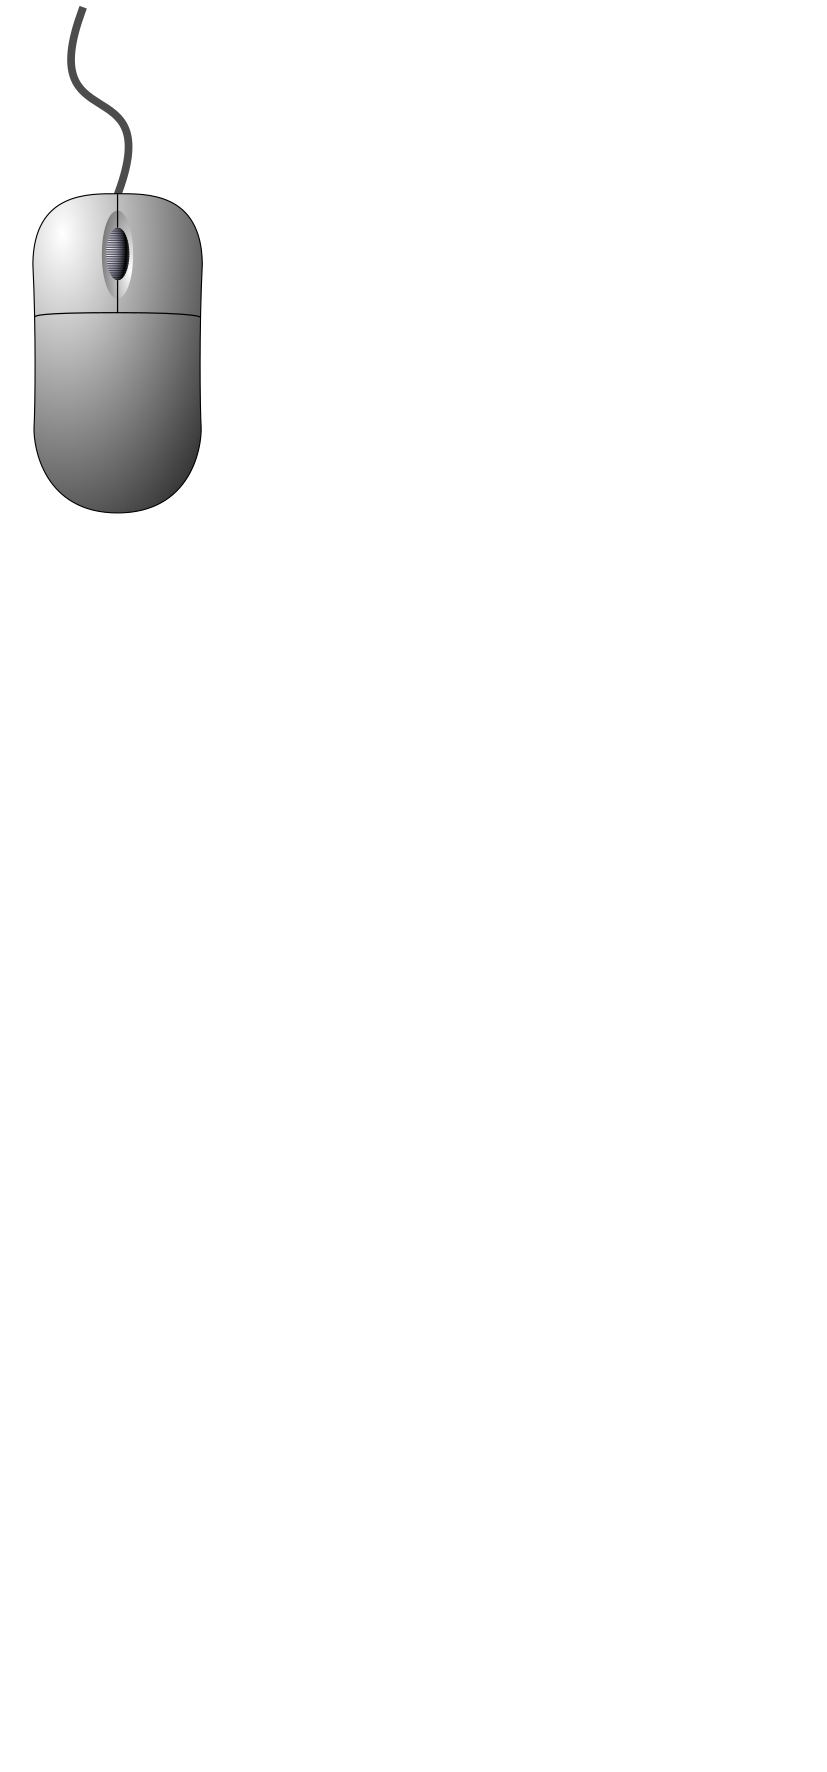
\includegraphics[keepaspectratio, height=30mm]{../../asset/image/textbook-img076.eps}
%     % \newline
%     % \small{2. SDカード}
%     % \newline
%   \end{minipage}
%   %
%   \begin{minipage}[b]{0.32\linewidth}
%     \centering
%     \textbf{右 クリック}
%     \newline
%     カチッ
%     \newline
%     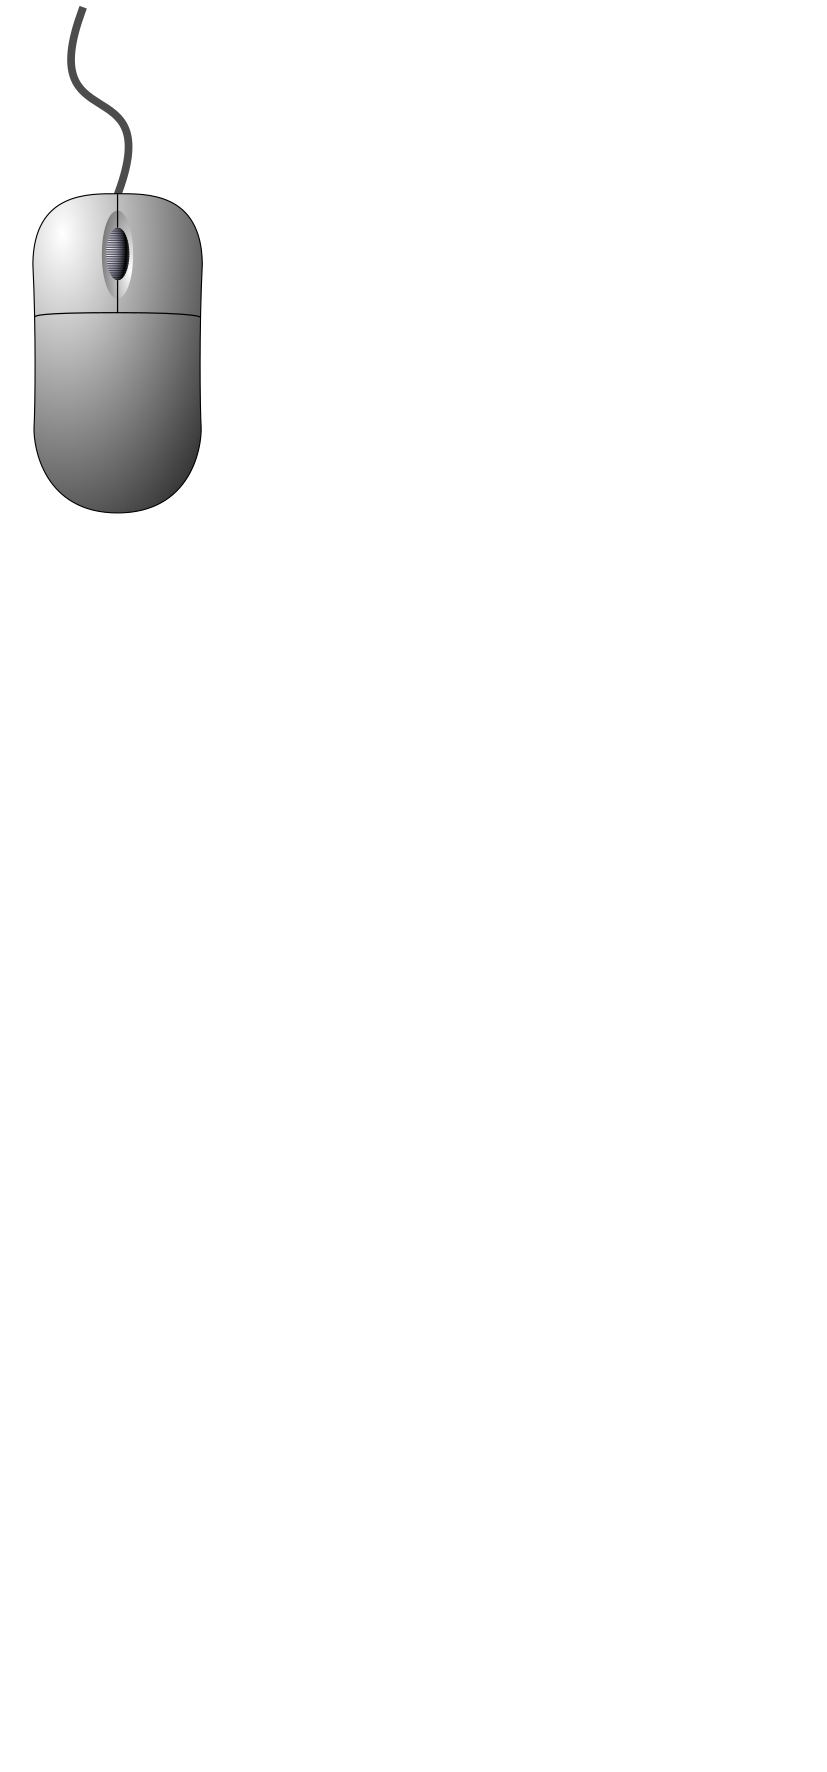
\includegraphics[keepaspectratio, height=30mm]{../../asset/image/textbook-img076.eps}
%     % \newline
%     % \small{3. 電源ケーブル}
%     % \newline
%   \end{minipage}
%   \label{fig:20}
%   %
% \end{figure}


% %後で修正　上がそろわない
% \begin{figure}
%   \begin{tabular}{ccc}
%     \begin{minipage}{0.33\textwidth}
%       \centering
%       \textbf{（左）クリック}
%       \flushleft
  
%       カチッ\\
%       \centering
%       \raisebox{20mm}{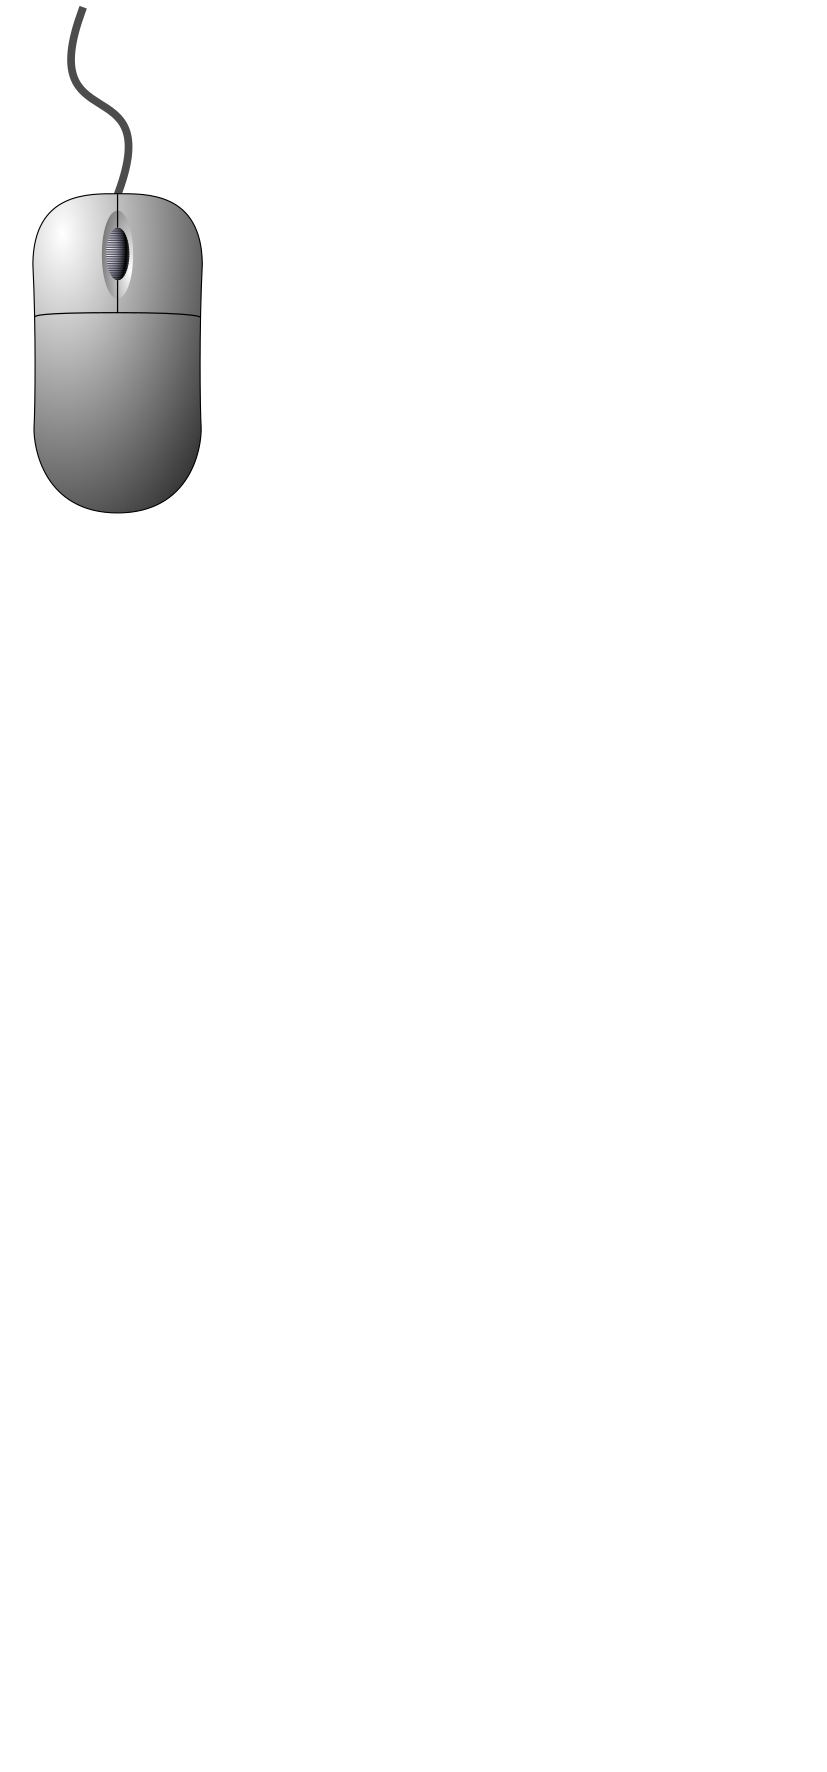
\includegraphics[width=1.651cm,height=3.53cm]{../../asset/image/textbook-img076.eps}}
  
%       \flushleft
%       マウスの左側を一度\ruby{押}{お}すこと、アプリなど開きたいときに使おう
%     \end{minipage}
  
%     \begin{minipage}{0.33\textwidth}
%       \centering
%       \textbf{ダブルクリック}
%       \flushleft
  
%       カチカチッ\\
%       \centering
%       \raisebox{20mm}{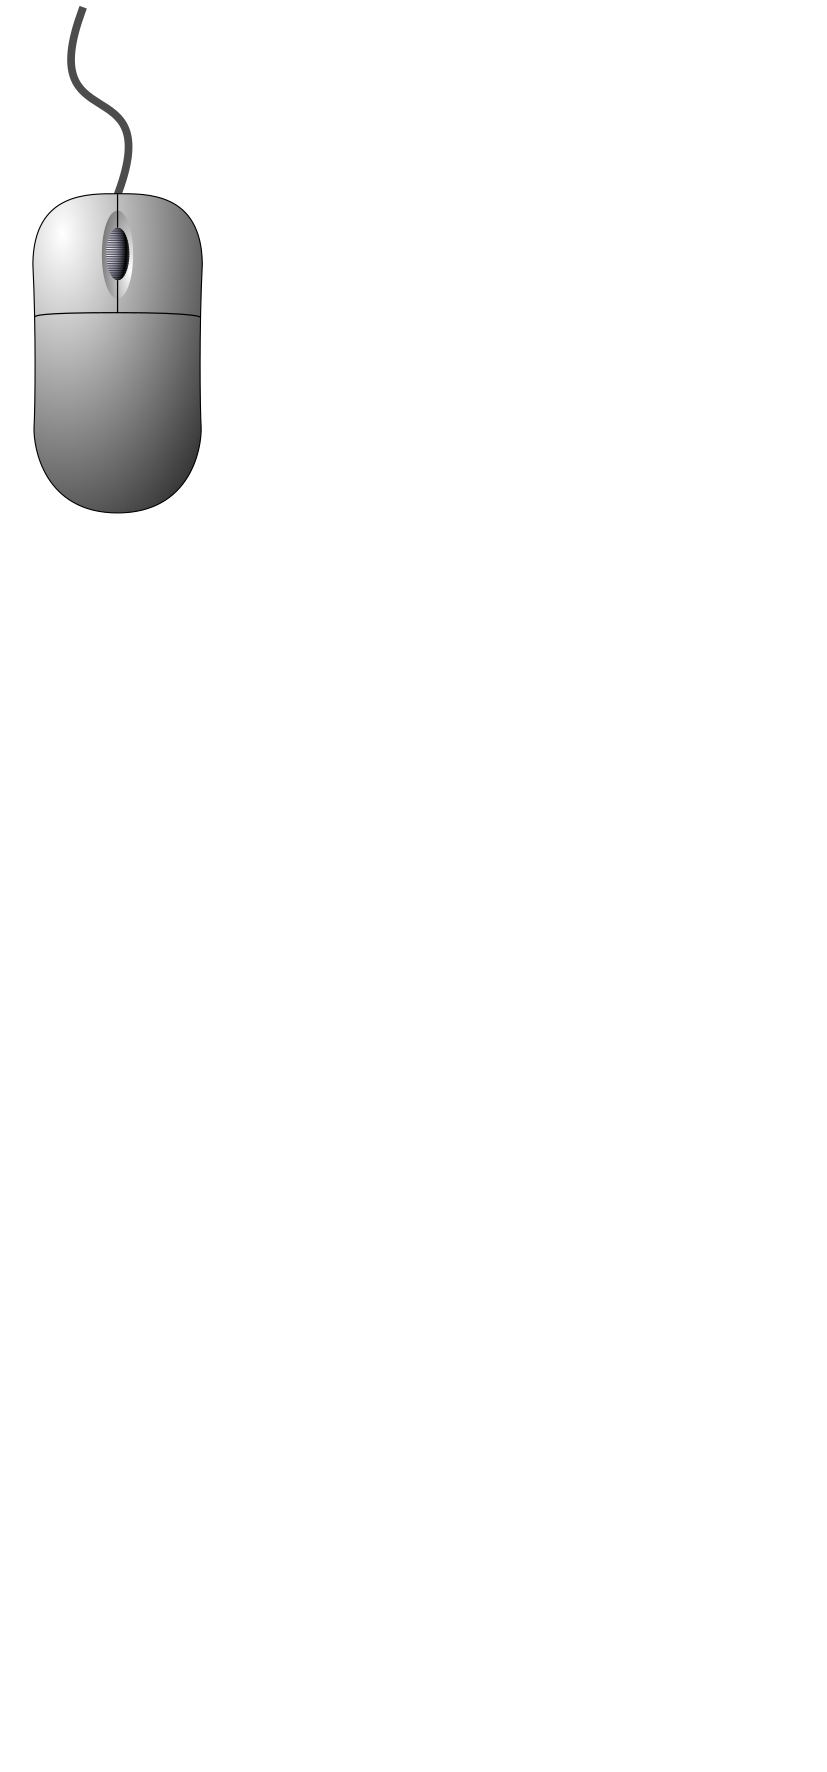
\includegraphics[width=1.651cm,height=3.53cm]{../../asset/image/textbook-img076.eps}}
  
%       \flushleft
%       マウスの左側を二回続けて\ruby{押}{お}すこと。　デスクトップのフォルダなどを開くときに使うよ
%     \end{minipage}
  
%     \begin{minipage}{0.33\textwidth}
%       \centering
%       \textbf{~~~~~右クリック}
%       \flushleft
  
%       \hspace{3cm} カチッ\\
%       \centering
%       \raisebox{20mm}{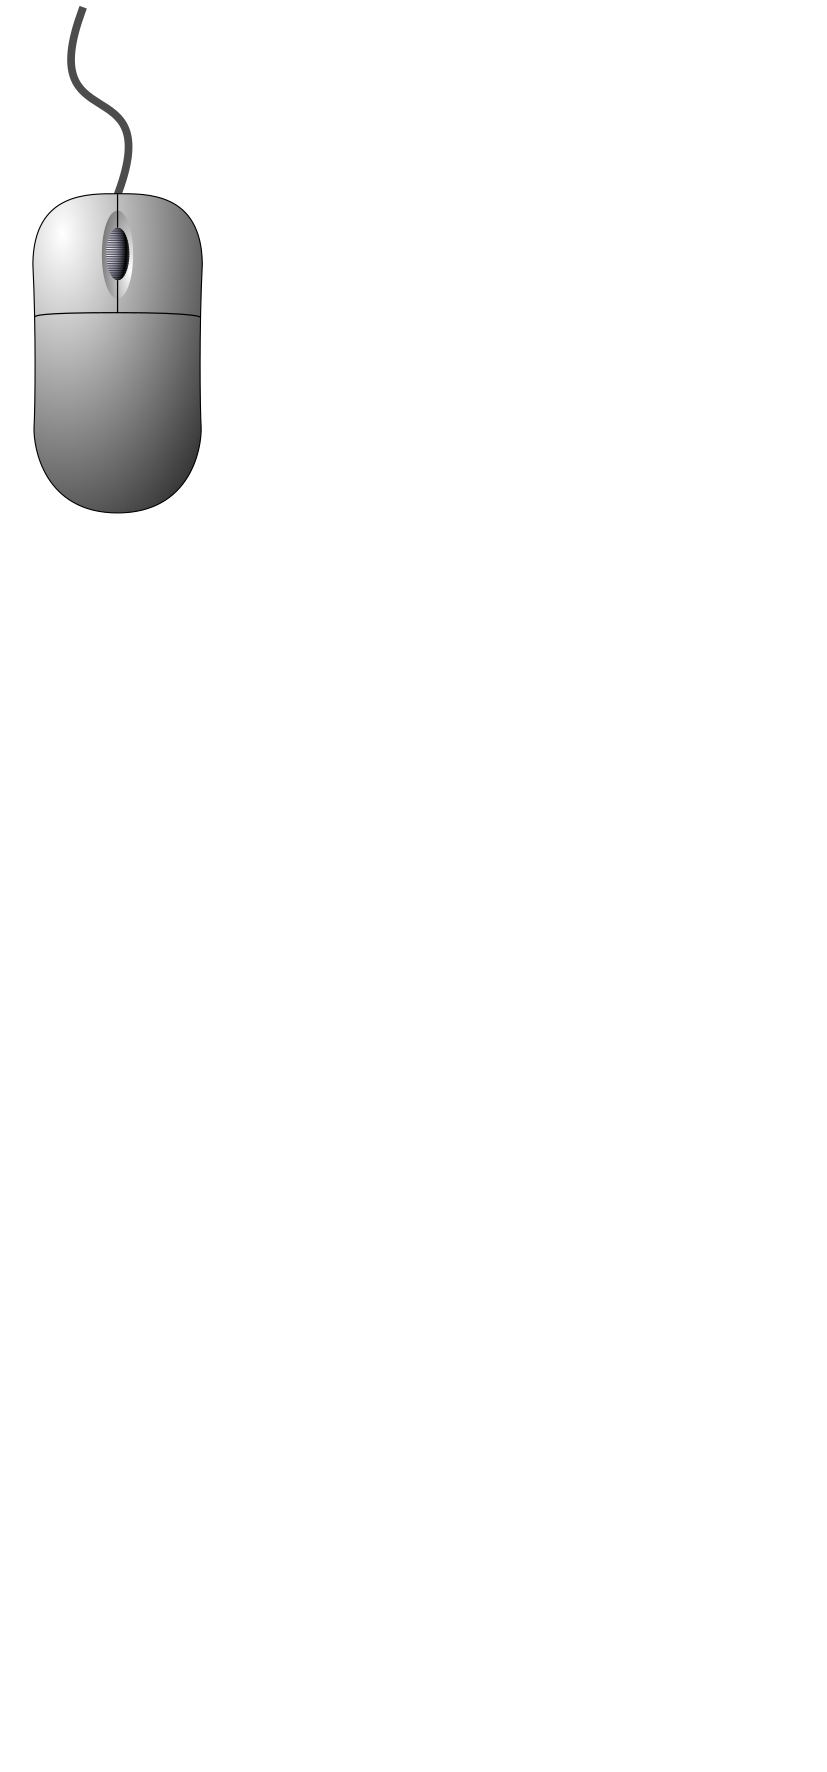
\includegraphics[width=1.651cm,height=3.53cm]{../../asset/image/textbook-img076.eps}}
  
%       \flushleft
%       マウスの右側を一度\ruby{押}{お}すこと。メニューなどを\ruby{表示}{ひょうじ}したいときに使うよ
%     \end{minipage}
    
%   \end{tabular}
% \end{figure}
% \clearpage



%
% subsubsection 1
%
\subsubsection{自分のフォルダを\ruby{確認}{かくにん}しよう}
\hrule\vspace*{5mm}

まず、みなさんがこの\ruby{授業}{じゅぎょう}で使う「自分のフォルダ」を\ruby{確認}{かくにん}しましょう。
さきほど、みなさんには「ユーザ名」と「パスワード」を\ruby{設定}{せってい}してもらいました。
そのとき\ruby{設定}{せってい}した「ユーザ名」によって、みなさんひとりひとりの「自分のフォルダ」の名前が変わります。
どこが変わるのか、じっさいに見てみましょう。\\

% \clearpage

{\bf 確認する手順}

% \begin{figure}[H]
  \begin{minipage}[t]{0.49\columnwidth}
    % \vspace*{-30mm}
    \textcircled{\scriptsize{1}}\\
    ディスプレイ左上の黄色いアイコン（ファイルマネージャ）をクリック
  \end{minipage}\hfill
  %
  \begin{minipage}[t]{0.49\columnwidth}
    \centering
    \vbox to 0pt{\vskip-3mm
      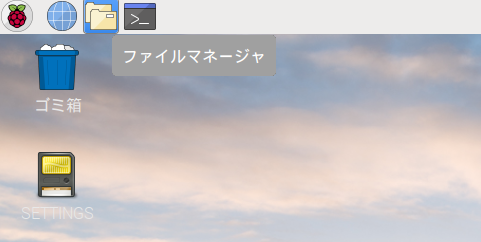
\includegraphics[keepaspectratio, height=30mm]{../../asset/image/textbook-img032.png}
    \vss}
    \vspace{40mm}
  \end{minipage}
  %
% \end{figure}
%

% \begin{figure}[H]
  \begin{minipage}[t]{0.49\linewidth}
    \textcircled{\scriptsize{2}}\\
    ファイルマネージャーが開いて、自分のフォルダの中が\ruby{表示}{ひょうじ}されます。
    （ウィンドウの色が\ruby{違}{ちが}うかもしれませんが、色はあとで変えられます。）
  \end{minipage}\hfill
  %
  \begin{minipage}[t]{0.49\linewidth}
    \centering
    \vbox to 0pt{\vskip-3mm
      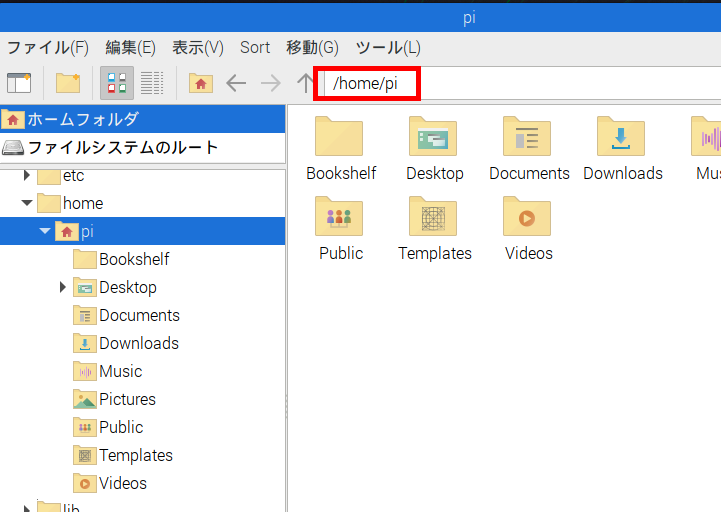
\includegraphics[keepaspectratio, height=50mm]{../../asset/image/textbook-img1020.png}
    \vss}
    \vspace{60mm}
  \end{minipage}
% \end{figure}
%


% {\bf \large 考え方}\\
% \begin{figure}[ht]
%   \begin{minipage}{\textwidth}
%     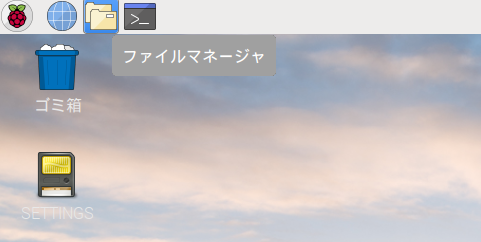
\includegraphics[width=0.4\textwidth]{../../asset/image/textbook-img032.png}
%     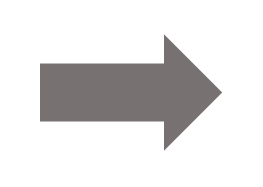
\includegraphics[width=2cm]{../../asset/image/textbook-img035.png}
%     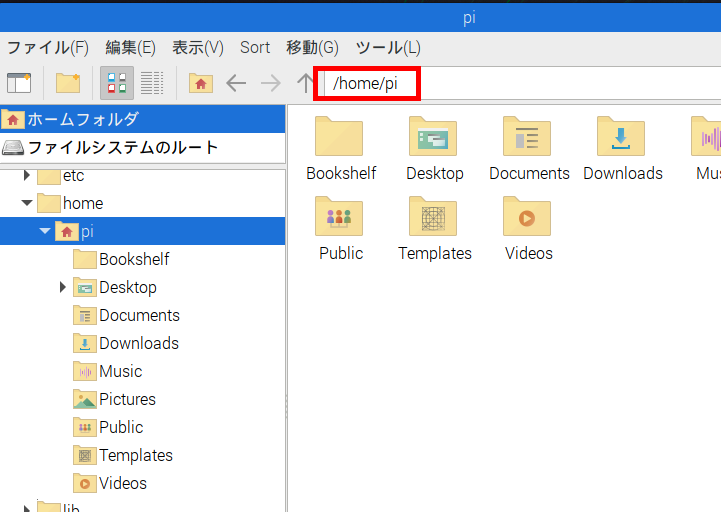
\includegraphics[width=0.5\textwidth]{../../asset/image/textbook-img1020.png}
%   \end{minipage}
%   \begin{minipage}{0.4\textwidth}
%     1
%     ディスプレイの左上の、黄色いアイコンをクリック
%   \end{minipage}
%   \hspace{2cm}
%   \vspace{20pt}
%   \begin{minipage}{0.5\textwidth}
%     \vspace{20pt}
%     2
%     ファイルマネージャーが開いて、自分のフォルダが\ruby{表示}{ひょうじ}されます。（ウィンドウの色が\ruby{違}{ちが}うかもしれませんが、色はあとで変えられます）
%   \end{minipage}
% \end{figure}

% \noindent

ファイルマネージャーのウィンドウの左側には、フォルダがツリー\ruby{表示}{ひょうじ}されます。
右側には、ツリーで選択されているフォルダ内のファイルが\ruby{表示}{ひょうじ}されます。
ファイルマネージャーは、\ruby{起動}{きどう}すると、\ruby{最初}{さいしょ}に自分のフォルダを\ruby{表示}{ひょうじ}します。
赤\ruby{枠}{わく}で囲まれたところに、自分のフォルダのパスが書いてあります。
パスについての\ruby{詳}{くわ}しい説明は、\ruby{以降}{いこう}の回で出てくるので、
今はとりあえずフォルダ、ファイルの「住所」と考えてください。
この例では、\verb|/home/pi|と表示されていますが、みなさんの場合は\ruby{違}{ちが}うパスが表示されていると思います。
\textbf{\color{red}ここに、最初に\ruby{設定}{せってい}した「ユーザ名」が反映されます。}
例えば、「\verb|chiba|」というユーザ名を\ruby{設定}{せってい}した場合は、赤\ruby{枠}{わく}の中に、
\verb|/home/chiba| と表示されます。
\vspace{20pt}

\begin{tcolorbox}[title=\useOmetoi,breakable]
  自分のフォルダのパスを見てみよう。
  \begin{enumerate}
    \addquiz{自分のフォルダのパスを下の\ruby{記入欄}{きにゅうらん}に記入してみましょう。}
  \end{enumerate}
\end{tcolorbox}
\clearpage


% \noindent \textbf{問題 1-6}\\
% 自分のフォルダのパス（右上の\ruby{画像}{がぞう}の赤い\ruby{枠}{わく}で囲まれた部分）を、下の\ruby{空欄}{くうらん}に書き写してみよう\\
% \vskip\baselineskip
% \underline{答え：\hspace{13.5cm}}
% \clearpage


%
% subsubsection 2
%
\subsubsection{フォルダを作成しよう}
\hrule\vspace*{5mm}

\texttt{Documents}フォルダの中に\texttt{taro}という名前のフォルダを作成しましょう。\\

{\bf 作成する手順}

% \begin{figure}[H]
  \begin{minipage}[t]{0.44\columnwidth}
    % \vspace*{-30mm}
    \textcircled{\scriptsize{1}}\\
    ウィンドウマネージャーの左側で、自分のフォルダの中の\texttt{Documents}フォルダをクリックした後、
    右側の空白部分で右クリックして、「New Folder」にカーソルを合わせてクリックする
  \end{minipage}\hfill
  %
  \begin{minipage}[t]{0.55\columnwidth}
    \centering
    \vbox to 0pt{\vskip-3mm
      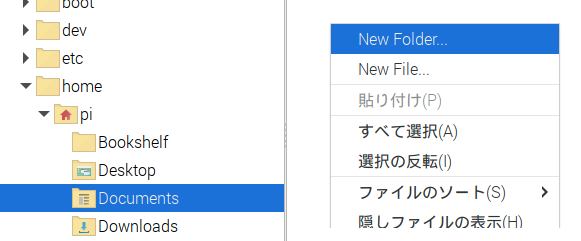
\includegraphics[keepaspectratio, height=35mm]{../../asset/image/textbook-img034x.png}
    \vss}
    \vspace{45mm}
  \end{minipage}
  %
% \end{figure}
%

% \begin{figure}[H]
\begin{minipage}[t]{0.44\columnwidth}
  % \vspace*{-30mm}
  \textcircled{\scriptsize{2}}\\
  フォルダの新規作成ウィンドウが表示されるので、テキストボックスに作成したいフォルダの名前（\texttt{taro}）を入力してOKをクリックする
\end{minipage}\hfill
%
\begin{minipage}[t]{0.55\columnwidth}
  \centering
  \vbox to 0pt{\vskip-3mm
    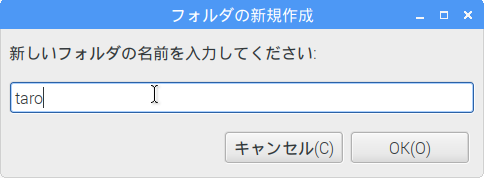
\includegraphics[keepaspectratio, height=30mm]{../../asset/image/textbook-img039x.png}
  \vss}
  \vspace{40mm}
\end{minipage}
%
% \end{figure}
%

% \begin{figure}[H]
\begin{minipage}[t]{0.44\columnwidth}
  % \vspace*{-30mm}
  \textcircled{\scriptsize{3}}\\
  入力した名前（\texttt{taro}）のフォルダが作成できていることを確認しよう
\end{minipage}\hfill
%
\begin{minipage}[t]{0.55\columnwidth}
  \centering
  \vbox to 0pt{\vskip-3mm
    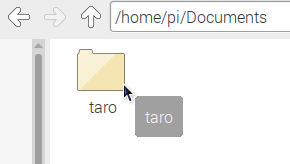
\includegraphics[keepaspectratio, height=30mm]{../../asset/image/textbook-img040x.png}
  \vss}
  \vspace{40mm}
\end{minipage}
%
% \end{figure}
%

たくさんのファイルをあつかう場合、フォルダはとても大切です。
フォルダには、\ruby{画像}{がぞう}やプログラムのコードなど、いろいろなファイルを\ruby{保存}{ほぞん}しておきますので、
わかりやすく\ruby{関係性}{かんけいせい}のある名前を付けてあげましょう。
なお、ファイルやフォルダの名前には、プログラムからあつかいやすいように、空白の入らない半角のアルファベットを使いましょう。
\vspace{20pt}

\begin{tcolorbox}[title=\useOmetoi,breakable]
  % 上の説明と同じ方法で、新しいフォルダを作成してみよう。
  \begin{enumerate}
    \addex{\texttt{Desktop}フォルダの中に、\texttt{space1}という名前のフォルダを作りましょう。}
    \addex{\texttt{Desktop}フォルダの中に、\texttt{space2}という名前のフォルダを作りましょう。}
    % \addex{Desktopフォルダの中に、\verb*space1*という名前のフォルダを作りましょう。}
    % \addex{Desktopフォルダの中に、\verb*space2*という名前のフォルダを作りましょう。}
  \end{enumerate}

\end{tcolorbox}



% {\bf \large 考え方}
% \begin{figure}[ht]
%   \centering
%   \begin{minipage}{0.9\textwidth}
%     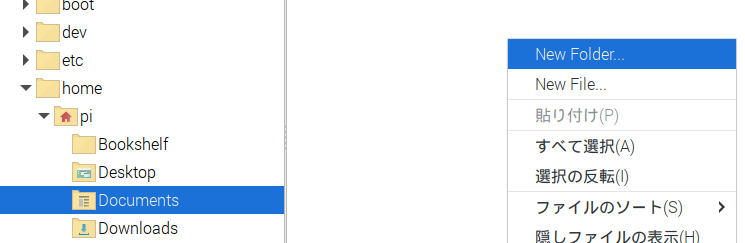
\includegraphics[width=\linewidth]{../../asset/image/textbook-img034.png}
%     1 ファイルマネージャーの空白部分で右クリックし、「New Folder」にカーソルを合わせてクリック
%      \vspace{60pt}
%   \end{minipage}

%   \centering
%   \begin{minipage}{0.9\textwidth}
%     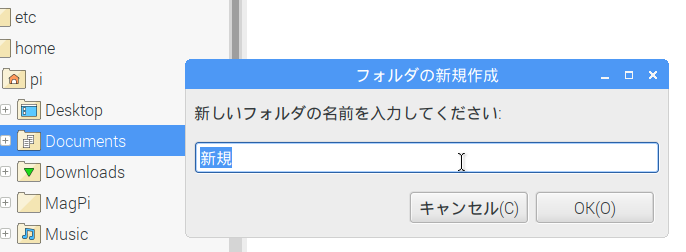
\includegraphics[width=\linewidth]{../../asset/image/textbook-img036.png}
%     2 フォルダ名の入力を求められるので、付けたい名前を入力しよう
%   \end{minipage}
% \end{figure}
% \clearpage




% {\bf\large 考え方(続き)}
% \begin{figure}[hb]
%   \centering
%   \begin{minipage}{0.9\textwidth}
%   %[Warning: Image ignored] % Unhandled or unsupported graphics:
%    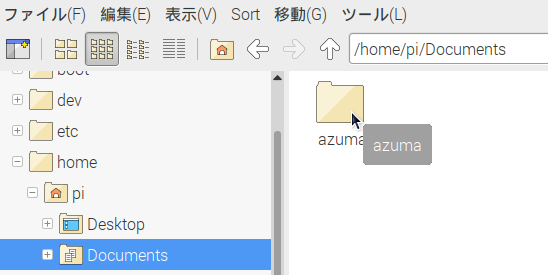
\includegraphics[width=\linewidth]{../../asset/image/textbook-img038.png}
%     3 名前を入力し、OKを\ruby{押}{お}すと上の\ruby{画像}{がぞう}のようにフォルダが作成されます
%   \end{minipage}
% \end{figure}


% \begin{figure}[hb]
%   \centering
%   \begin{minipage}{0.9\textwidth}
%     {	\large
%       フォルダは大事です。

%       フォルダに、\ruby{画像}{がぞう}やプログラムのコードを\ruby{保存}{ほぞん}しておくので、わかりやすく\ruby{関係性}{かんけいせい}のある名前を付けてあげましょう
%       \vskip.5\baselineskip
%       ファイルやフォルダの名前は、空白の入らない半角ローマ字にしておくと、後でプログラムから使う時に便利だよ
%     }
%   \end{minipage}
% \end{figure}
% \clearpage

% \begin{figure}[ht]
%   \flushleft{\bf\large 答え}
%   \vspace{8mm}\\
%   \centering
%   \begin{minipage}{0.8\textwidth}
%    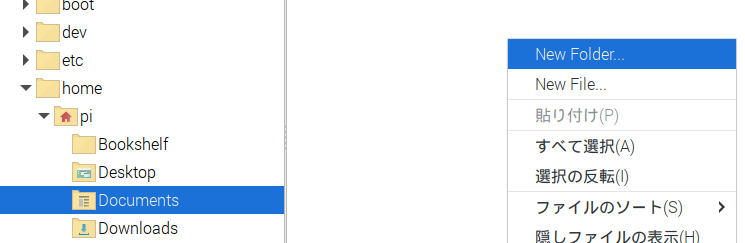
\includegraphics[width=\linewidth]{../../asset/image/textbook-img034.png}
%     1
%     \ 左上のフォルダアイコンをクリックし

%     フォルダマネージャー上で右クリックし、上の\ruby{画像}{がぞう}のようにしよう
%   \end{minipage}
%   \vspace{\baselineskip}

%   \centering
%   %[Warning: Image ignored] % Unhandled or unsupported graphics:
%   \begin{minipage}{0.8\textwidth}
%    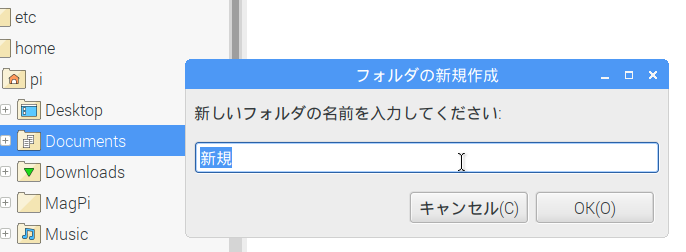
\includegraphics[width=\linewidth]{../../asset/image/textbook-img036.png}
%     2
%     \ 「New Folder」を選び、名前\ruby{設定}{せってい}に行こう
%   \end{minipage}
%   \vspace{\baselineskip}

%   \centering
%   %[Warning: Image ignored] % Unhandled or unsupported graphics:
%   \begin{minipage}{0.8\textwidth}
%   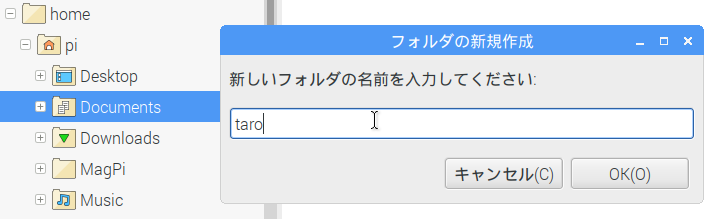
\includegraphics[width=\linewidth]{../../asset/image/textbook-img039.png}
%     3
%     \ taroと名前を入力し、OKを\ruby{押}{お}す
%   \end{minipage}
%   \vspace{\baselineskip}

%   \centering
%   %[Warning: Image ignored] % Unhandled or unsupported graphics:
%   \begin{minipage}{0.8\textwidth}
%   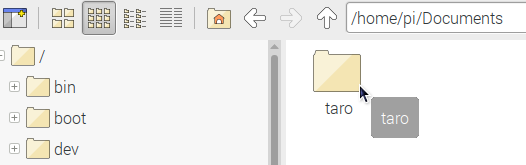
\includegraphics[width=\linewidth]{../../asset/image/textbook-img040.png}
%     4
%     \ taroというフォルダを作成できていることを\ruby{確認}{かくにん}しよう
%   \end{minipage}

% \end{figure}
% \clearpage



% \begin{figure}
%   \flushleft{\bf\large
%     答え(続き)}\\
%   \vspace{10mm}
%   \centering
%   %[Warning: Image ignored] % Unhandled or unsupported graphics:
%   \begin{minipage}{0.8\textwidth}
%   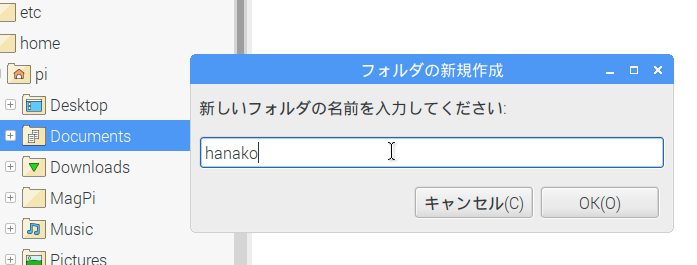
\includegraphics[width=\linewidth]{../../asset/image/textbook-img041.png}
%     5
%     \ 先ほどと同じように右クリックから「New Folder」を選び、hanakoという名前でフォルダを作成
%   \end{minipage}
%   \vspace{\baselineskip}

%   \centering
%   %[Warning: Image ignored] % Unhandled or unsupported graphics:
%   \begin{minipage}{0.8\textwidth}
%   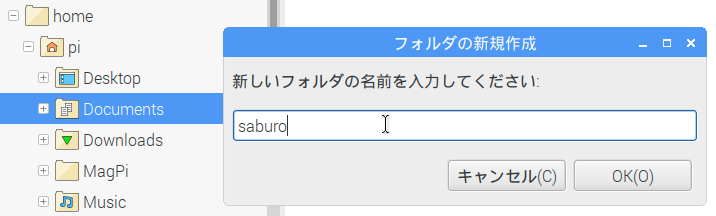
\includegraphics[width=\linewidth]{../../asset/image/textbook-img042.png}
%     6
%     \ saburoというフォルダを先ほどと同じ方法で作成
%   \end{minipage}
%   \vspace{\baselineskip}

%   \centering
%   %[Warning: Image ignored] % Unhandled or unsupported graphics:
%   \begin{minipage}{0.8\textwidth}
%   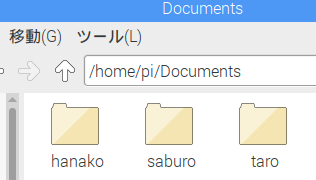
\includegraphics[width=\linewidth]{../../asset/image/textbook-img043.png}
%     7 
%     \ taro , hanako , saburoのフォルダが作成されていることを\ruby{確認}{かくにん}してみよう
%   \end{minipage}
%   \vspace{10mm}
%   \flushleft

%   \noindent \textbf{問題 1-7}\\
%   例題と同じ方法で、akahoshi、imaoka、hamanakaという名前のフォルダを作ろう
%   % \refstepcounter{Question}\theQuestion\label{Q:hasAnswer02-1}

%   % 例題と同じ方法で、akahoshi、imaoka、hamanakaという名前のフォルダを作ろう

% \end{figure}
% \clearpage


%
% subsubsection 3
%
\subsubsection{フォルダを\ruby{移動}{いどう}しよう}
\hrule\vspace*{5mm}

まずは、\texttt{Desktop}フォルダの中にある\texttt{space1}フォルダの中に、新しく\texttt{move}フォルダを作ります。
そして、この\texttt{move}フォルダを\texttt{space2}フォルダの中に移動します。
（\texttt{space1}と\texttt{space2}は、直前の問題で作成したフォルダです。）\\

{\bf フォルダを移動する手順}

\begin{minipage}[t]{0.49\columnwidth}
  \textcircled{\scriptsize{1}}\\
  ウィンドウ左側の\texttt{Desktop}をクリックして、\texttt{space1}と\texttt{space2}フォルダがあることを確認する（フォルダがない時は、作成してください）
\end{minipage}\hfill
%
\begin{minipage}[t]{0.49\columnwidth}
  \centering
  \vbox to 0pt{\vskip-3mm
    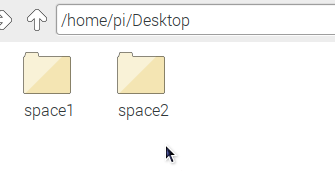
\includegraphics[keepaspectratio, height=30mm]{../../asset/image/textbook-img051.png}
  \vss}
  \vspace{35mm}
\end{minipage}


\begin{minipage}[t]{0.49\columnwidth}
  \textcircled{\scriptsize{2}}\\
  \texttt{sapce1}をダブルクリックして\texttt{space1}の中に移動し、\texttt{move}フォルダを作成する
\end{minipage}\hfill
%
\begin{minipage}[t]{0.49\columnwidth}
  \centering
  \vbox to 0pt{\vskip-3mm
    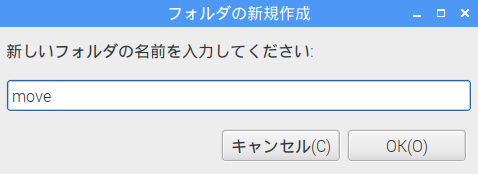
\includegraphics[keepaspectratio, height=25mm]{../../asset/image/textbook-img050.png}
  \vss}
  \vspace{35mm}
\end{minipage}


\begin{minipage}[t]{0.49\columnwidth}
  \textcircled{\scriptsize{3}}\\
  \texttt{move}フォルダ上で右クリックして、メニューから切り取りをクリックする
\end{minipage}\hfill
%
\begin{minipage}[t]{0.49\columnwidth}
  \centering
  \vbox to 0pt{\vskip-3mm
    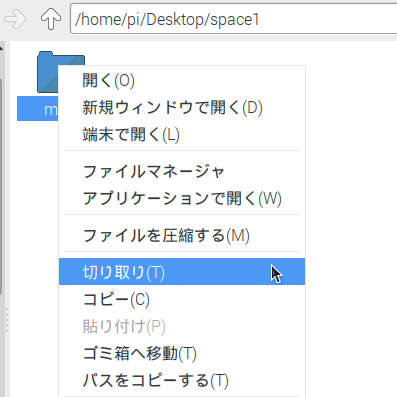
\includegraphics[keepaspectratio, height=55mm]{../../asset/image/textbook-img048x.png}
  \vss}
  \vspace{60mm}
\end{minipage}


\begin{minipage}[t]{0.49\columnwidth}
  \textcircled{\scriptsize{4}}\\
  \texttt{sapce2}をダブルクリックして\texttt{space2}の中に移動し、右側の空白部分で右クリックして、メニューから\ruby{貼}{は}り付けをクリックする
\end{minipage}\hfill
%
\begin{minipage}[t]{0.49\columnwidth}
  \centering
  \vbox to 0pt{\vskip-3mm
    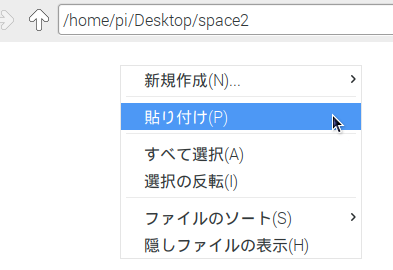
\includegraphics[keepaspectratio, height=40mm]{../../asset/image/textbook-img046xx.png}
  \vss}
  \vspace{45mm}
\end{minipage}


\begin{minipage}[t]{0.49\columnwidth}
  \textcircled{\scriptsize{5}}\\
  これで、\texttt{space1}の中にあった\texttt{move}フォルダが\texttt{sapce2}の中に移動しました
\end{minipage}\hfill
%
\begin{minipage}[t]{0.49\columnwidth}
  \centering
  \vbox to 0pt{\vskip-3mm
    % 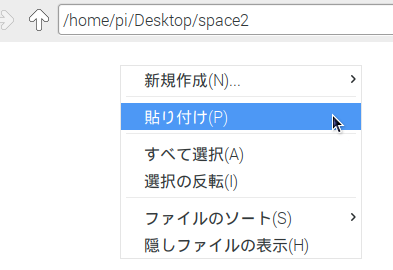
\includegraphics[keepaspectratio, height=40mm]{../../asset/image/textbook-img046xx.png}
  \vss}
  \vspace{20mm}
\end{minipage}
% \vspace{20pt}

\begin{tcolorbox}[title=\useOmetoi,breakable]
  \begin{enumerate}
    \addex{\texttt{space1}フォルダの中に、\texttt{rasp}という名前のフォルダを作り、さらにそのフォルダ内に\texttt{berry}という名前のフォルダを作成しよう。}
    \addex{\texttt{rasp}フォルダを\texttt{space2}フォルダの中に移動して、その中身を確認しよう。}
  \end{enumerate}

\end{tcolorbox}



% \begin{figure}[htbp]
%   \subsection{例題 1-7 フォルダを\ruby{移動}{いどう}しよう}
%   Desktop直下に「space1」と「space2」を作り、「space1」の中に「move」フォルダを作り、「move」フォルダを「space2」に\ruby{移動}{いどう}しよう

%   \flushleft{\bf\large 考え方} 
%   \centering
%   %[Warning: Image ignored] % Unhandled or unsupported graphics:
%   \includegraphics[width=0.8\textwidth]{../../asset/image/fig15-1.eps}
%   \begin{minipage}{15.297cm}
%     フォルダやファイルは後からでも動かすことができるよ。
%   \end{minipage}

%   % \begin{minipage}{5.963cm}
%   \begin{minipage}{0.4\textwidth}
%     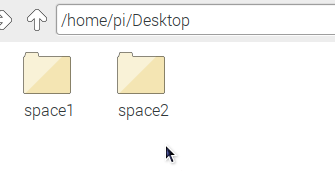
\includegraphics[width=\linewidth]{../../asset/image/textbook-img051.png}
%     {\flushleft
%       1 左側のDesktopをクリックし、space1とspace2を作成
%     }
%   \end{minipage}
%   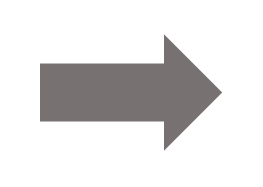
\includegraphics[width=2cm]{../../asset/image/textbook-img052.png}
%   \begin{minipage}{0.4\textwidth}
%     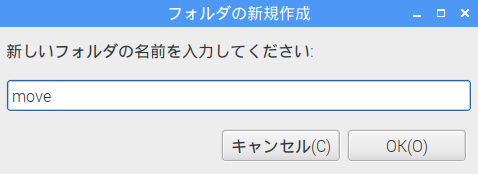
\includegraphics[width=\linewidth]{../../asset/image/textbook-img050.png}
%     {\flushleft
%       2 space1の中にmoveフォルダを作成
%     }
%   \end{minipage}

%   \centering
%   \begin{minipage}{0.4\textwidth}
%     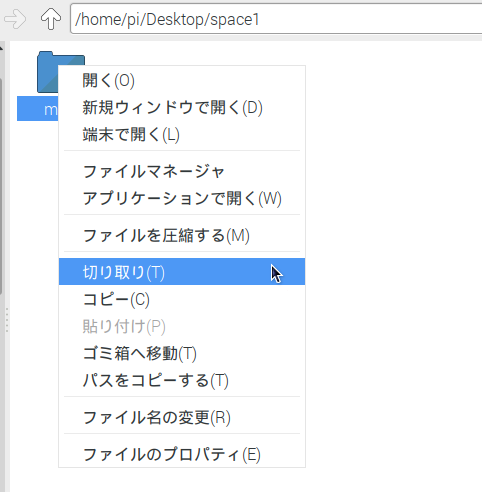
\includegraphics[width=\linewidth]{../../asset/image/textbook-img048.png}
%     {\flushleft
%       3 moveフォルダ上で右クリックし、切り取りをクリック
%     }
%   \end{minipage}
%   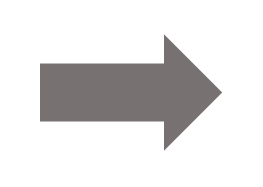
\includegraphics[width=2cm]{../../asset/image/textbook-img049.png}
%   \begin{minipage}{0.4\textwidth}
%     %
\includegraphics[width=2.168cm,height=1.542cm]{textbook-img047.png}
%     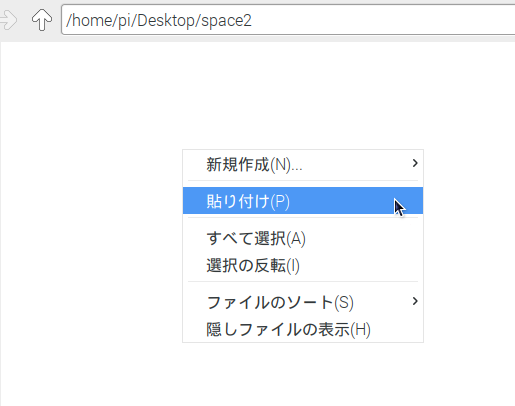
\includegraphics[width=\linewidth]{../../asset/image/textbook-img046.png}
%     {\flushleft
%       4 space2の中で右クリック、\ruby{貼}{は}り付けをクリック
%     }
%   \end{minipage}

%   %[Warning: Image ignored] % Unhandled or unsupported graphics:
%   \begin{minipage}{6.589cm}
%     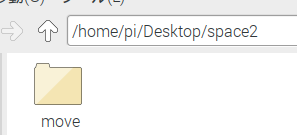
\includegraphics[width=7.218cm]{../../asset/image/textbook-img045.png}
%     {\flushleft
%       5 space1の中にあったmoveフォルダがspace2に\ruby{移動}{いどう}しました
%     }
%   \end{minipage}

%   \flushleft
%   \noindent \textbf{問題 1-8}\\
%   「space1」フォルダ内に「rasp」フォルダを作り、さらにそのフォルダ内に「berry」フォルダを作成して「rasp」フォルダを「space2」フォルダに\ruby{移動}{いどう}させよう。そして中身を\ruby{確認}{かくにん}しよう
  
% \end{figure}

% \clearpage






%
% subsubsection 4
%
\subsubsection{ファイル名・フォルダ名を\ruby{変更}{へんこう}しよう}
\hrule\vspace*{5mm}


\texttt{before}という名前のフォルダを\texttt{Documents}直下に作り、作成した後でそのフォルダ名を\texttt{after}に変えよう。
ファイル名もフォルダ名も同じ手順で変えることができます。
これは、間違えたファイル名・フォルダ名を変えたいときなどに使います。\\

{\bf ファイル名・フォルダを変更する手順}

\begin{minipage}[t]{0.49\columnwidth}
  \textcircled{\scriptsize{1}}\\
  ウィンドウ左側の\texttt{Documents}をクリックして、\texttt{before}フォルダを作成する
\end{minipage}\hfill
%
\begin{minipage}[t]{0.49\columnwidth}
  \centering
  \vbox to 0pt{\vskip-3mm
    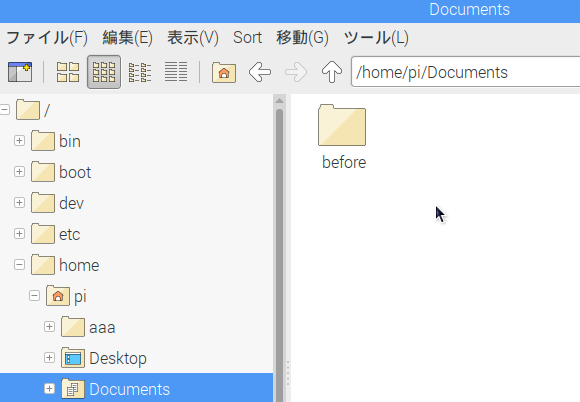
\includegraphics[keepaspectratio, height=45mm]{../../asset/image/textbook-img058.png}
  \vss}
  \vspace{50mm}
\end{minipage}

\begin{minipage}[t]{0.49\columnwidth}
  \textcircled{\scriptsize{2}}\\
  \texttt{before}フォルダ上で右クリックして、メニューからファイル名の変更をクリック
\end{minipage}\hfill
%
\begin{minipage}[t]{0.49\columnwidth}
  \centering
  \vbox to 0pt{\vskip-3mm
    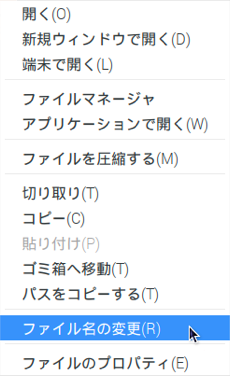
\includegraphics[keepaspectratio, height=45mm]{../../asset/image/textbook-img057x.png}
  \vss}
  \vspace{50mm}
\end{minipage}

\begin{minipage}[t]{0.49\columnwidth}
  \textcircled{\scriptsize{3}}\\
  名前を\texttt{after}に変更してOKをクリック
\end{minipage}\hfill
%
\begin{minipage}[t]{0.49\columnwidth}
  \centering
  \vbox to 0pt{\vskip-3mm
    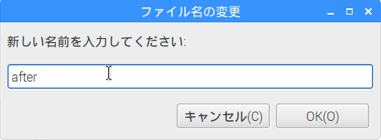
\includegraphics[keepaspectratio, height=25mm]{../../asset/image/textbook-img055x.png}
  \vss}
  \vspace{30mm}
\end{minipage}

\begin{tcolorbox}[title=\useOmetoi,breakable]
  \begin{enumerate}
    \addex{\texttt{Documents}フォルダの中に、\texttt{wrong}という名前のフォルダを作り、その後でフォルダ名を\texttt{correct}に変えよう。}
  \end{enumerate}
\end{tcolorbox}



% \begin{figure}[ht]
%   \flushleft{\bf\large 考え方}

%   \centering
%   %[Warning: Image ignored] % Unhandled or unsupported graphics:
%   \begin{minipage}{1.978cm}
%     
\includegraphics[width=1.5cm]{../../asset/image/textbook-img044.png}
%     frog
%   \end{minipage}
%   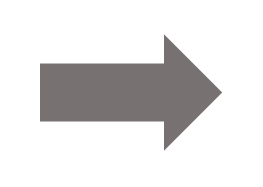
\includegraphics[width=2cm]{../../asset/image/textbook-img052.png}
%   \begin{minipage}{1.978cm}
%     
\includegraphics[width=1.5cm]{../../asset/image/textbook-img044.png}
%     dog
%   \end{minipage}
%   \begin{minipage}{6.319cm}
%     まちがったフォルダ名をつけたとき、名前を変えたいときなどに使います。
%   \end{minipage}

%   \begin{minipage}{0.4\textwidth}
%     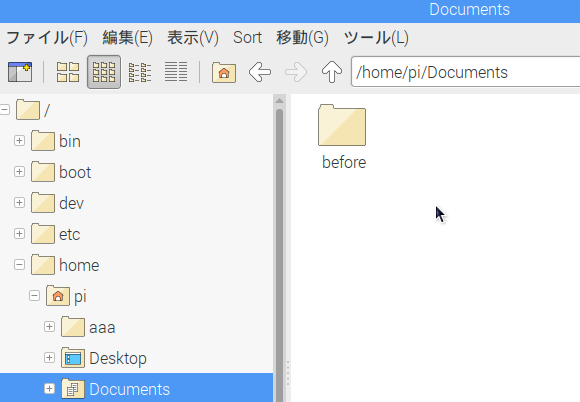
\includegraphics[width=\linewidth]{../../asset/image/textbook-img058.png}
%     \flushleft
%     1 左側のDocumentsをクリックし「before」フォルダを作成
%   \end{minipage}
%   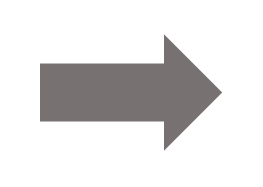
\includegraphics[width=2cm]{../../asset/image/textbook-img052.png}
%   \begin{minipage}{0.4\textwidth}
%     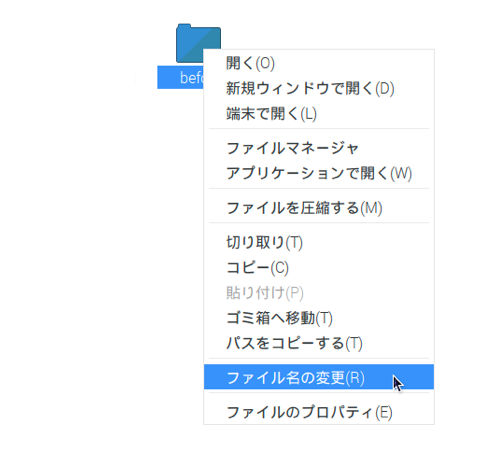
\includegraphics[width=\linewidth]{../../asset/image/textbook-img057.png}
%     \flushleft
%     2 フォルダ上で右クリックし、

%     ファイル名の\ruby{変更}{へんこう}をクリック
%   \end{minipage}
%   %[Warning: Image ignored] % Unhandled or unsupported graphics:

%   \begin{minipage}{0.4\textwidth}
%     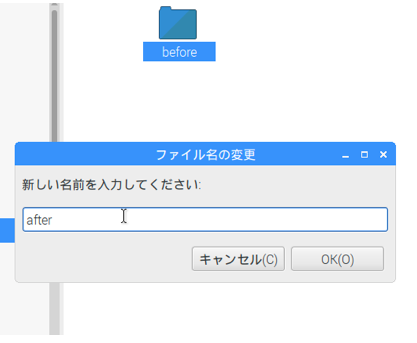
\includegraphics[width=\linewidth]{../../asset/image/textbook-img055.png}
%     3 名前を「after」に\ruby{変更}{へんこう}

%     OKをクリック
%   \end{minipage}
%   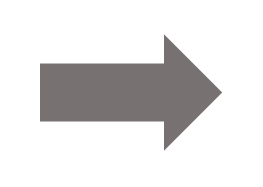
\includegraphics[width=2cm]{../../asset/image/textbook-img053.png}
%   \begin{minipage}{0.4\textwidth}
%     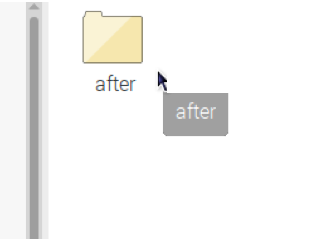
\includegraphics[width=\linewidth]{../../asset/image/textbook-img056.png}
%     4 変更を\ruby{確認}{かくにん}
%   \end{minipage}
%   \centering

%   \begin{minipage}{5.751cm}
%     フォルダ名の\ruby{変更}{へんこう}は、よく使うので覚えておこう
%   \end{minipage}

%   \flushleft
%   \noindent \textbf{問題 1-9}\\
%   miss\_name」という名前のフォルダを１つ作り、その作成した後でフォルダ名を「success\_name」に変えよう

% \end{figure}


\clearpage

%
% subsection 1.2.2
%
\subsection{文字の入力}

テキストエディタ（Mousepad）を開き、アルファベットをa〜zまで入力しましょう。
その後で、「こんにちは」「こんばんは」「ごきげんよう」「さようなら」「ありがとう」をそれぞれ一行に入力しましょう。
日本語を入力するときには、英字入力モードから日本語入力モードに切り\ruby{替}{か}える必要があります。
英字入力と日本語入力のモードを切り\ruby{替}{か}えるには、下図の赤わくで囲んだCtrlキーとスペースキーを同時に\ruby{押}{お}します。

\begin{figure}[hb]
  \centering
    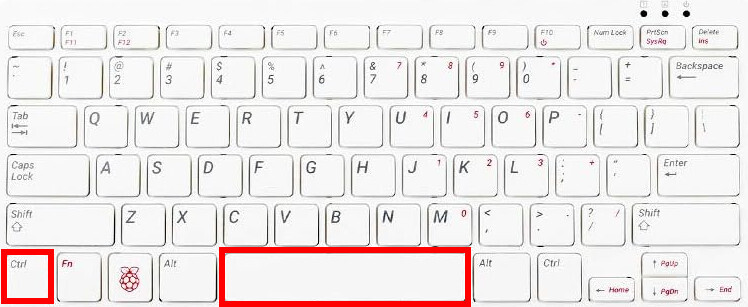
\includegraphics[keepaspectratio, height=40mm]{../../asset/image/2024_keyboard.jpg}
    \caption{入力モードの切り替え}
    \label{fig:20}
\end{figure}




{\bf 文字入力の手順}

\begin{minipage}[t]{0.49\columnwidth}
  \textcircled{\scriptsize{1}}\\
  左上のラズベリーのアイコンをクリックして表示されるメニューから、[アクセサリ]->[Text Editor（Mousepad）]をクリックします
\end{minipage}\hfill
%
\begin{minipage}[t]{0.49\columnwidth}
  \centering
  \vbox to 0pt{\vskip-3mm
    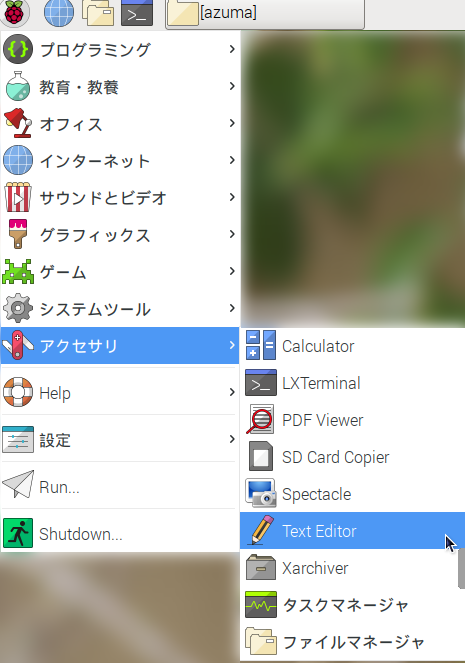
\includegraphics[keepaspectratio, height=45mm]{../../asset/image/textbook-img064x.png}
  \vss}
  \vspace{50mm}
\end{minipage}

\begin{minipage}[t]{0.49\columnwidth}
  \textcircled{\scriptsize{2}}\\
  テキストエディタのウィンドウをクリックして、左上（右図の赤線）のカーソルが\ruby{点滅}{てんめつ}していることを確認してください
\end{minipage}\hfill
%
\begin{minipage}[t]{0.49\columnwidth}
  \centering
  \vbox to 0pt{\vskip-3mm
    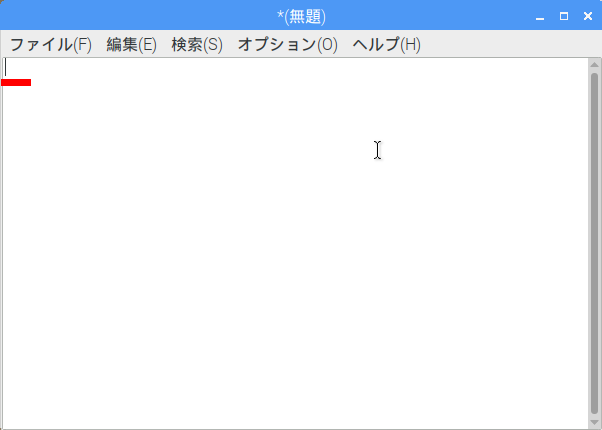
\includegraphics[keepaspectratio, height=40mm]{../../asset/image/textbook-img063.png}
  \vss}
  \vspace{45mm}
\end{minipage}

\begin{minipage}[t]{0.49\columnwidth}
  \textcircled{\scriptsize{3}}\\
  Ctrlキーを\ruby{押}{お}しながらスペースキーを\ruby{押}{お}して文字入力を切り替えよう
  （タスクバーの右上のアイコンが、英字入力の場合は「キーボード」アイコンに、日本語入力の場合は「あ」アイコンに\ruby{替}{か}わります）
\end{minipage}\hfill
%
\begin{minipage}[t]{0.49\columnwidth}
  \centering
  \vbox to 0pt{\vskip-3mm
    % 
\includegraphics[keepaspectratio, width=0.8\columnwidth]{../../asset/image/textfig_001.png}
    % 
\includegraphics[keepaspectratio, width=0.8\columnwidth]{../../asset/image/textfig_002.png}
    
\includegraphics[scale=0.8]{../../asset/image/textfig_001.png}
    
\includegraphics[scale=0.8]{../../asset/image/textfig_002.png}
  \vss}
  \vspace{35mm}
\end{minipage}

\begin{minipage}[t]{0.49\columnwidth}
  \textcircled{\scriptsize{4}}\\
  まずはアルファベットを入力したいので、「キーボード」アイコンに切り\ruby{替}{か}えて、a～zまで入力しよう
\end{minipage}\hfill
%
\begin{minipage}[t]{0.49\columnwidth}
  \centering
  \vbox to 0pt{\vskip-3mm
    % 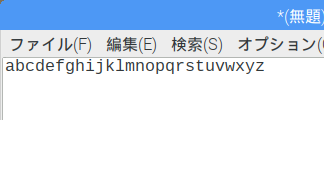
\includegraphics[keepaspectratio, height=33mm]{../../asset/image/textbook-img061x.png}
    % 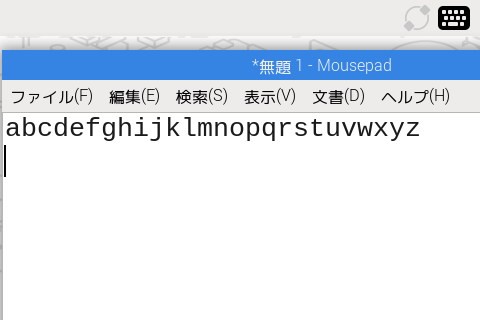
\includegraphics[keepaspectratio, width=0.7\columnwidth]{../../asset/image/textfig_003.png}
    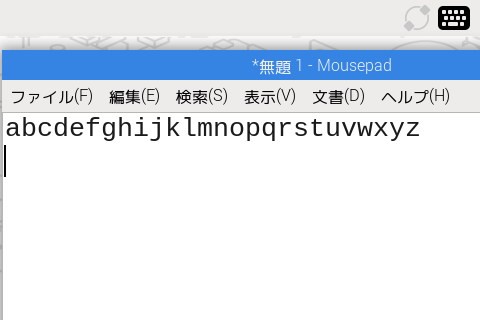
\includegraphics[scale=0.5]{../../asset/image/textfig_003.png}
  \vss}
  \vspace{45mm}
\end{minipage}

\begin{minipage}[t]{0.49\columnwidth}
  \textcircled{\scriptsize{5}}\\
  次に日本語を入力したいので、「あ」アイコンに切り\ruby{替}{か}えて、こんにちは～ありがとうまでを入力しよう
\end{minipage}\hfill
%
\begin{minipage}[t]{0.49\columnwidth}
  \centering
  \vbox to 0pt{\vskip-3mm
    % 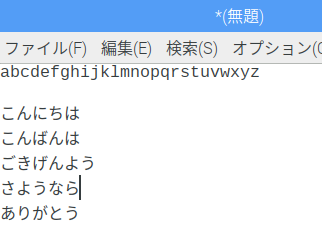
\includegraphics[keepaspectratio, height=40mm]{../../asset/image/textbook-img060.png}
    % 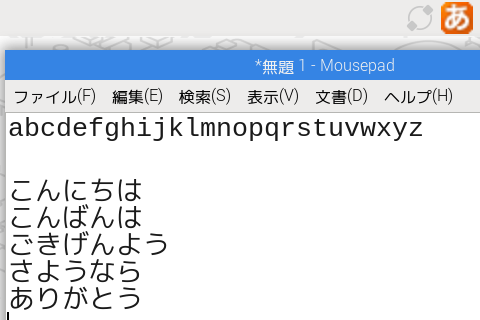
\includegraphics[keepaspectratio, width=0.7\columnwidth]{../../asset/image/textfig_004.png}
    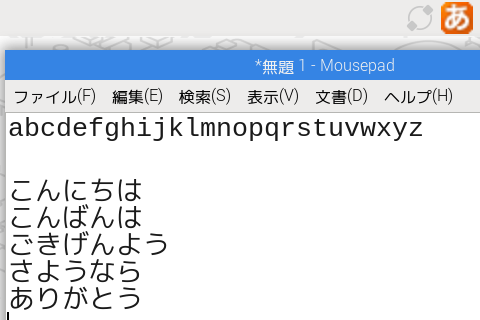
\includegraphics[scale=0.5]{../../asset/image/textfig_004.png}
  \vss}
  \vspace{45mm}
\end{minipage}

\begin{tcolorbox}[title=\useOmetoi,breakable]
  \begin{enumerate}
    \addex{テキストエディタで\texttt{A}～\texttt{Z}を入力しよう（ヒント：大文字を入力するにはshiftキーを\ruby{押}{お}しながらアルファベットキーを打つ）。}
  \end{enumerate}
\end{tcolorbox}



% \begin{figure}[ht]
%   \subsection{例題 1-9 日本語入力と英字入力について}
%   \flushleft
%   Mousepadを開き、アルファベットをa〜zまで入力しよう。その後「こんにちは」「こんばんは」「ごきげんよう」「さようなら」「ありがとう」をそれぞれ一行に入力しましょう。
  
%   {\bf\large 考え方}

%   \centering
%   \begin{minipage}{\textwidth}
%     % 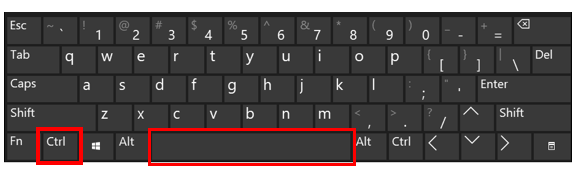
\includegraphics[width=0.4\textwidth]{../../asset/image/textbook-img065.png}
%     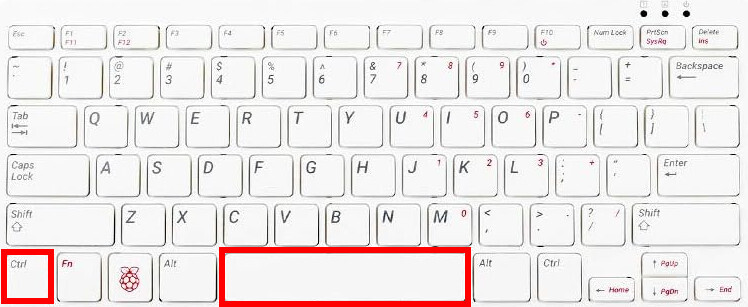
\includegraphics[width=0.4\textwidth]{../../asset/image/2024_keyboard.jpg}
%     \raisebox{10mm}
%     {
%       \begin{minipage}{0.5\textwidth}
%         赤わくで囲んだCtrlとスペースを同時に\ruby{押}{お}すことで
%         英字入力と日本語入力を切り\ruby{替}{か}えることができるよ
%       \end{minipage}
%     }
%   \end{minipage}

%   \begin{minipage}{0.3\textwidth}
%     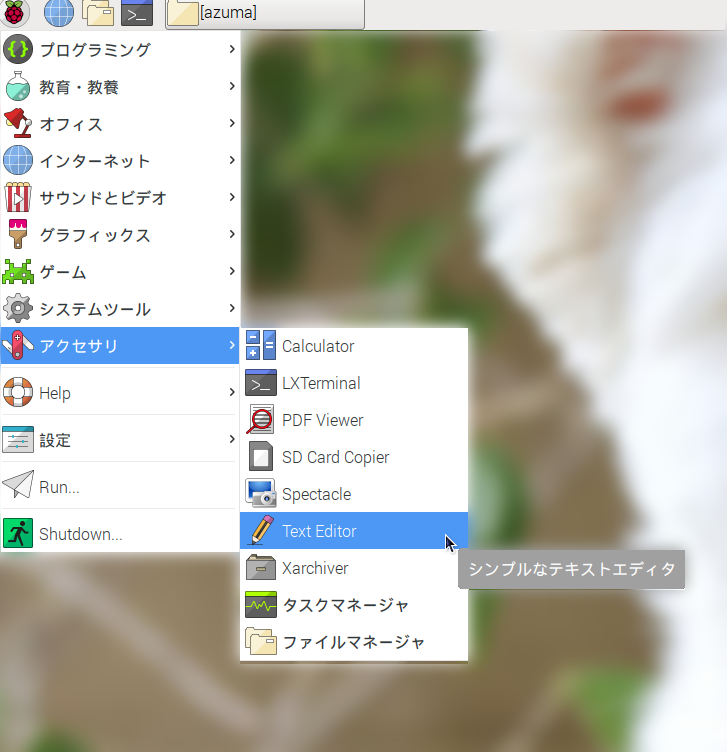
\includegraphics[width=\linewidth]{../../asset/image/textbook-img064.png}
%     \flushleft
%     1 ラズベリーのアイコンをクリックしてアクセサリー＞Text editorを開こう
%   \end{minipage}
%   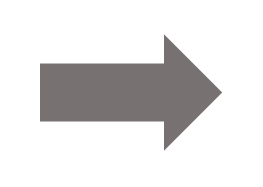
\includegraphics[width=2cm]{../../asset/image/textbook-img053.png}
%   \begin{minipage}{0.4\textwidth}
%     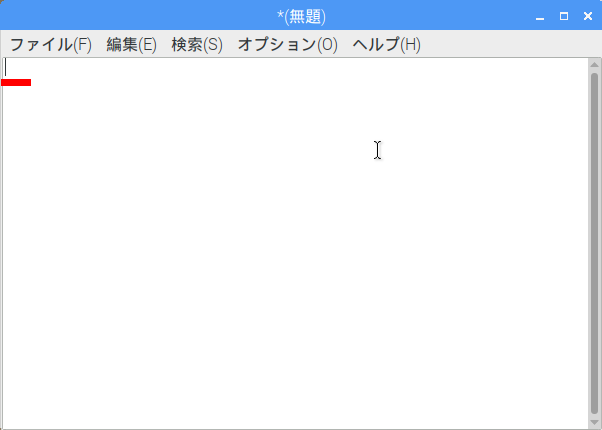
\includegraphics[width=\linewidth]{../../asset/image/textbook-img063.png}
%     \flushleft
%     2 赤線が引かれているところをクリックしてテキストエディタにカーソル（\ruby{縦棒}{たてぼう}）が入っていることを\ruby{確認}{かくにん}してください。
%   \end{minipage}

%   \begin{minipage}{0.4\textwidth}
%     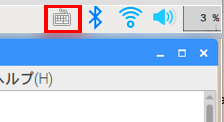
\includegraphics[width=\linewidth]{../../asset/image/textbook-img059.png}
%     \flushleft
%     3 Ctrlとスペースキーを同時に\ruby{押}{お}して

%     英字入力に切り\ruby{替}{か}えよう。アイコンがキーボードであることを\ruby{確認}{かくにん}しよう。
%   \end{minipage}
%   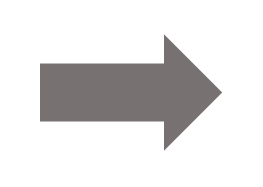
\includegraphics[width=2cm]{../../asset/image/textbook-img053.png}
%   \begin{minipage}{0.4\textwidth}
%     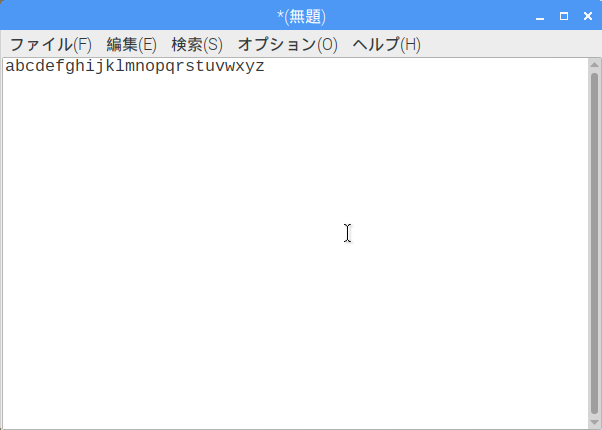
\includegraphics[width=\linewidth]{../../asset/image/textbook-img061.png}
%     \flushleft
%     4 英字入力でa〜zまで入力しよう
%   \end{minipage}

%   \begin{minipage}{0.4\textwidth}
%     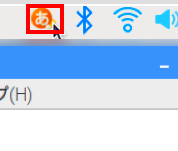
\includegraphics[width=\linewidth]{../../asset/image/textbook-img062.png}
%     \flushleft
%     5 Ctrlとスペースキーを同時に\ruby{押}{お}して
%     アイコンが“あ”になったか\ruby{確認}{かくにん}しましょう。
%   \end{minipage}
%   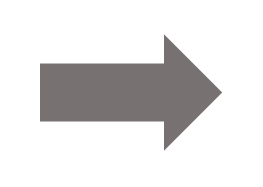
\includegraphics[width=2cm]{../../asset/image/textbook-img053.png}
%   \begin{minipage}{0.4\textwidth}
%     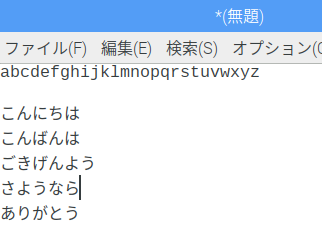
\includegraphics[width=\linewidth]{../../asset/image/textbook-img060.png}
%     \flushleft
%     6 こんにちは〜ありがとうを入力\\
%     7 完成
%   \end{minipage}
  
%   \flushleft
%   \noindent \textbf{問題 1-10}\\
%   Text editorでA〜Zを入力しよう
%   \noindent ヒント 
%   英字入力時にshiftキーを\ruby{押}{お}しながらアルファベットキーを打つと大文字で入力できます
% \end{figure}

% \clearpage

%
% subsubsection 1
%
\subsubsection{半角文字と全角文字について}
\hrule\vspace*{5mm}

全角文字とは、文字の縦と横の比率が1対1の文字のことを指します。
それに対して、半角文字は、横の幅が全角の半分（縦と横の比率が2対1）になります。
それでは、全角と半角の文字の違いを見てみましょう。


\begin{figure}[hb]
  \centering
    % 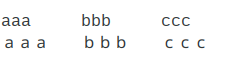
\includegraphics[keepaspectratio, height=20mm]{../../asset/image/textbook-img066.png}
    % 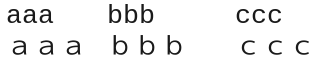
\includegraphics[keepaspectratio, width=0.5\columnwidth]{../../asset/image/textfig_005.png}
    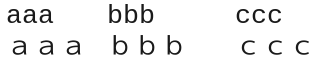
\includegraphics[scale=0.8]{../../asset/image/textfig_005.png}
    \caption{半角文字と全角文字（上：半角，下：全角）}
    \label{fig:21}
\end{figure}

ここで、上の行が半角で下の行が全角の例になります。
アルファベットのサイズからも分かる通り、横幅が大きい方が全角で、小さい方が半角だと覚えておいてください。
日本語の文字は（半角カタカナを除いて）すべて全角です。
なお、
\textbf{\color{red}{プログラミングでアルファベットや記号を入力するときは、必ず半角文字(小さい文字)を使いましょう}}。


% \begin{figure}
%   \subsection{例題 1-10 半角入力と全角入力について}
%   Text Editorを開き、半角入力でアルファベットをa〜zまで入力し、その後、全角入力で
%   アルファベットa〜zまで入力しよう。全角と半角文字の\ruby{違}{ちが}いを\ruby{理解}{りかい}しよう。

%   {\bf\large 考え方}

%   \centering
%   %[Warning: Image ignored] % Unhandled or unsupported graphics:
%   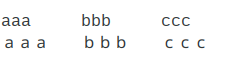
\includegraphics[width=5.978cm]{../../asset/image/textbook-img066.png}
%   \raisebox{8mm}{
%     \begin{minipage}{6.762cm}
%       {文字が小さいのが半角}\\
%       {文字が大きいのが全角}
%     \end{minipage}
%   }

%   \begin{minipage}{16.578cm}
%     % \bigskip
%     アルファベットのサイズからも分かる通り、大きいサイズが全角で、小さいサイズが半角だと覚えておくといいよ
%   \end{minipage}

%   \begin{minipage}{0.3\textwidth}
%     %[Warning: Image ignored] % Unhandled or unsupported graphics:
%     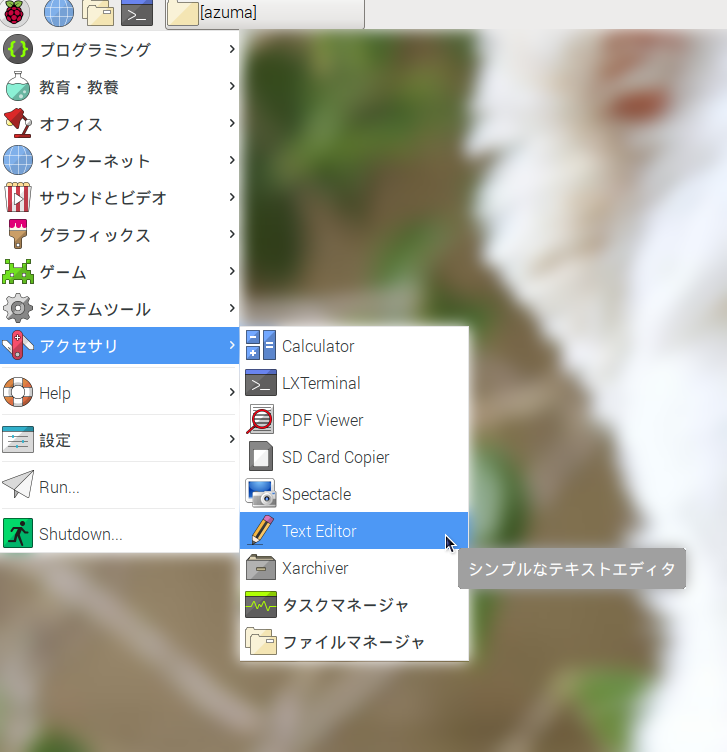
\includegraphics[width=\linewidth]{../../asset/image/textbook-img067.png}
%     \flushleft
%     1 Text editorを開こう
%   \end{minipage}
%   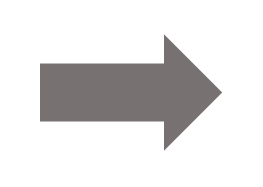
\includegraphics[width=2cm]{../../asset/image/textbook-img073.png}
%   \begin{minipage}{0.3\textwidth}
%     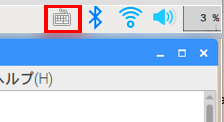
\includegraphics[width=\linewidth]{../../asset/image/textbook-img059.png}
%     \flushleft
%     2 キーボードのアイコンになっていることを\ruby{確認}{かくにん}して半角を入力しよう
%   \end{minipage}

%   \begin{minipage}{0.3\textwidth}
%     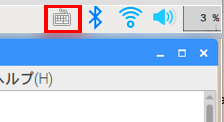
\includegraphics[width=\linewidth]{../../asset/image/textbook-img059.png}
%     \flushleft
%     3 半角のアルファベットを入力し終えたら右上のキーボードアイコンをクリック
%   \end{minipage}
%   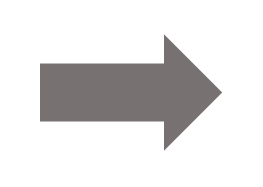
\includegraphics[width=2cm]{../../asset/image/textbook-img073.png}
%   \begin{minipage}{0.3\textwidth}
%     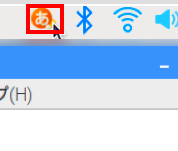
\includegraphics[width=\linewidth]{../../asset/image/textbook-img062.png}
%     \flushleft
%     4 アイコンが変わったことを\ruby{確認}{かくにん}しよう
%   \end{minipage}

%   \begin{minipage}{0.3\textwidth}
%     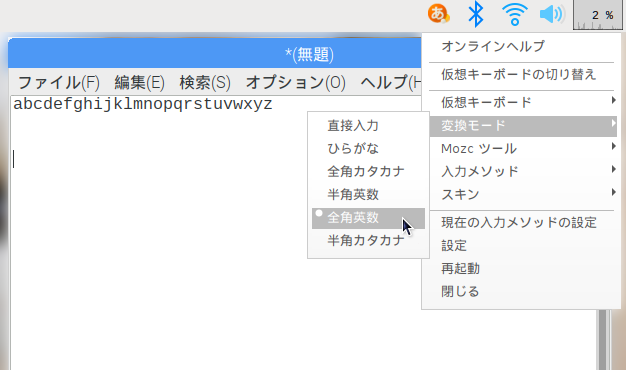
\includegraphics[width=\linewidth]{../../asset/image/textbook-img069.png}
%     \flushleft
%     5 アイコンを右クリックして、全角英数を\ruby{選択}{せんたく}
%   \end{minipage}
%   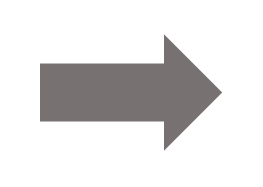
\includegraphics[width=2cm]{../../asset/image/textbook-img073.png}
%   \begin{minipage}{0.3\textwidth}
%     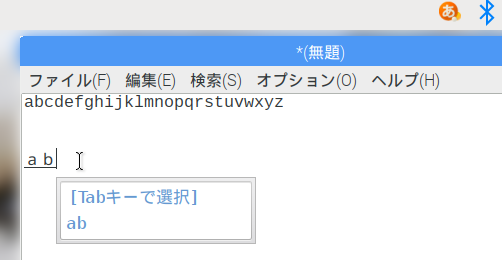
\includegraphics[width=\linewidth]{../../asset/image/textbook-img070.png}
%     \flushleft
%     6 入力
%   \end{minipage}

%   \vspace{3mm}
%   \begin{minipage}{\textwidth}
%     {\centering\textbf{\color{red}{
%       プログラミングでアルファベット,記号を入力するときは
%       半角(小さい文字)で入力しましょう}}
%     }
%   \end{minipage}

%   \flushleft
%   \noindent \textbf{問題1-11}\\
%   Text editorで半角A〜Zと全角A〜Zを入力しよう
%   ヒント

%   英字入力時にshiftキーを\ruby{押}{お}しながらアルファベットキーを打つと大文字で入力できます

% \end{figure}

\clearpage


%
% subsubsection 1
%
\subsubsection{ブラウザで\ruby{検索}{けんさく}しよう}
\hrule\vspace*{5mm}

ウェブブラウザ（ブラウザとも呼ばれます）を開いていろいろなことを\ruby{検索}{けんさく}してみましょう。
ブラウザを使用するとウェブサイトを開くことができます。
もし、困ったことがあったら自分で\ruby{検索}{けんさく}できるように使い方を覚えておきましょう。\\

{\bf \ruby{検索}{けんさく}の手順}

\begin{minipage}[t]{0.49\columnwidth}
  \textcircled{\scriptsize{1}}\\
  デスクトップ左上の地球儀のアイコンをクリックするとブラウザが起動します
\end{minipage}\hfill
%
\begin{minipage}[t]{0.49\columnwidth}
  \centering
  \vbox to 0pt{\vskip-3mm
    % 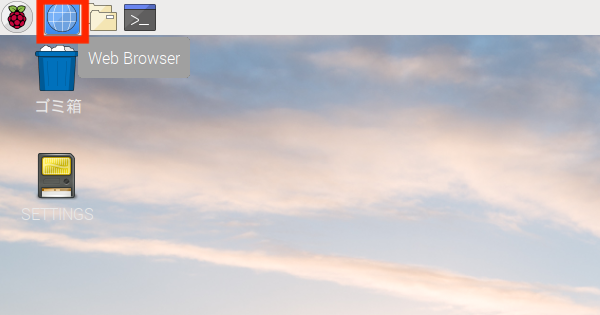
\includegraphics[keepaspectratio, height=30mm]{../../asset/image/textbook-img071.png}
    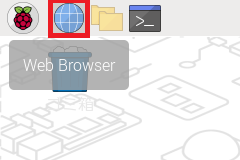
\includegraphics[scale=0.8]{../../asset/image/textfig_006.png}
  \vss}
  \vspace{35mm}
\end{minipage}

\begin{minipage}[t]{0.49\columnwidth}
  \textcircled{\scriptsize{2}}\\
  ブラウザが起動したら、赤で囲われている部分をクリックし、キーボードで\ruby{検索}{けんさく}したいワードを入力して
  Enterキーを押す
\end{minipage}\hfill
%
\begin{minipage}[t]{0.49\columnwidth}
  \centering
  \vbox to 0pt{\vskip-3mm
    % 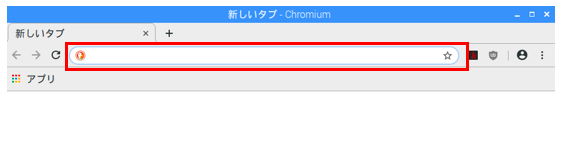
\includegraphics[keepaspectratio, height=20mm]{../../asset/image/textbook-img075.png}
    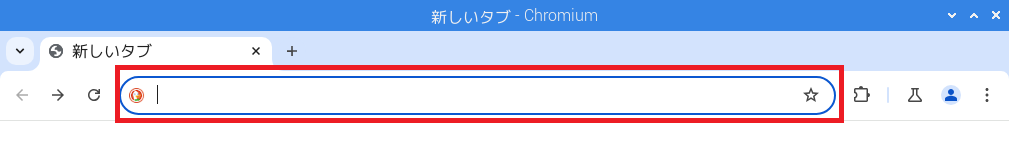
\includegraphics[scale=0.25]{../../asset/image/textfig_007.png}
  \vss}
  \vspace{20mm}
\end{minipage}
\vspace*{10mm}


{\bf 画像の\ruby{検索}{けんさく}}（「ねこ」の画像を\ruby{検索}{けんさく}してみよう）

\begin{minipage}[t]{0.49\columnwidth}
  \textcircled{\scriptsize{1}}\\
  ブラウザを起動して、「ねこ」と入力してEnterキーを押すと、「ねこ」の\ruby{検索}{けんさく}結果が表示されます
  % （著作権の関画像をぼかしています）
\end{minipage}\hfill
%
\begin{minipage}[t]{0.49\columnwidth}
  \centering
  \vbox to 0pt{\vskip-3mm
    % 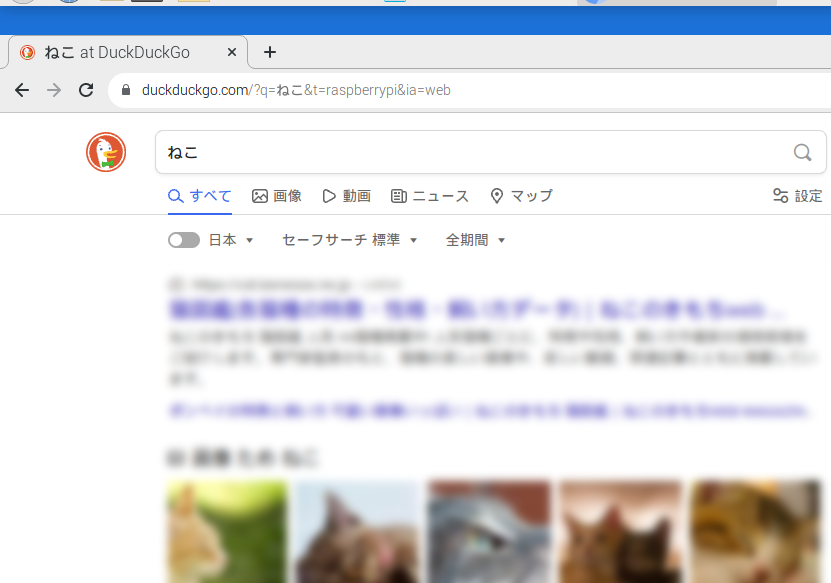
\includegraphics[keepaspectratio, height=40mm]{../../asset/image/textbook-img078x.png}
    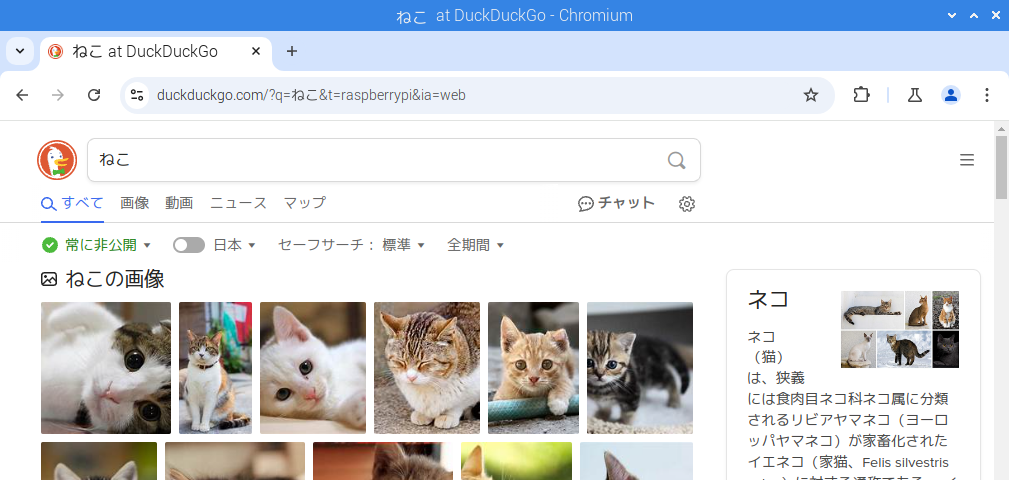
\includegraphics[scale=0.25]{../../asset/image/textfig_008.png}
  \vss}
  \vspace{40mm}
\end{minipage}

\begin{minipage}[t]{0.49\columnwidth}
  \textcircled{\scriptsize{2}}\\
  赤線で囲まれている「画像」をクリックすると、「ねこ」の画像だけが\ruby{検索}{けんさく}できます
  （「すべて」をクリックすると、もとの\ruby{検索}{けんさく}結果にもどります）
\end{minipage}\hfill
%
\begin{minipage}[t]{0.49\columnwidth}
  \centering
  \vbox to 0pt{\vskip-3mm
    % 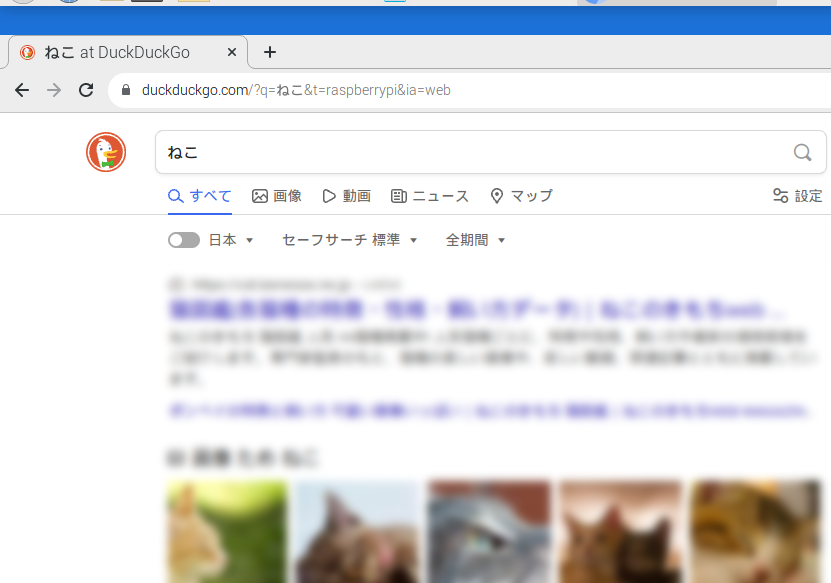
\includegraphics[keepaspectratio, height=40mm]{../../asset/image/textbook-img078x.png}
    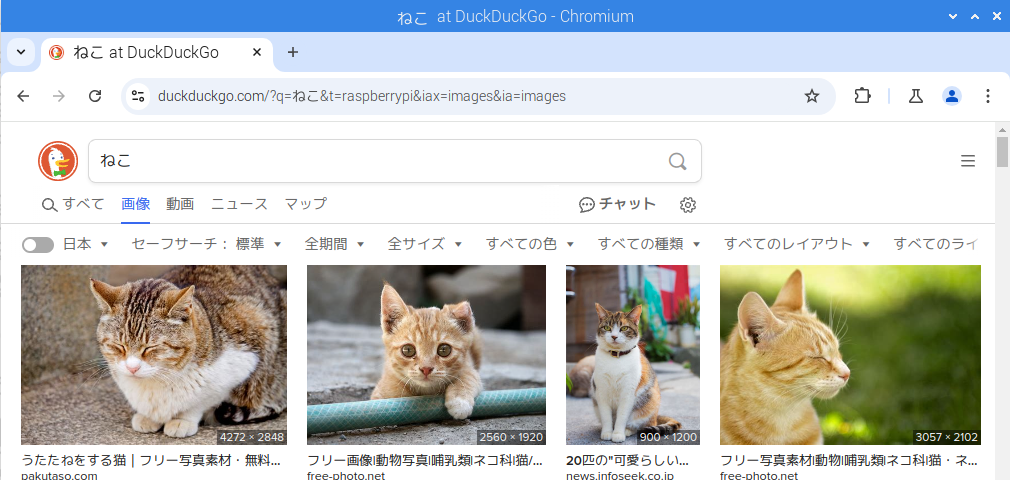
\includegraphics[scale=0.25]{../../asset/image/textfig_009.png}
  \vss}
  \vspace{45mm}
\end{minipage}

\begin{tcolorbox}[title=\useOmetoi,breakable]
  \begin{enumerate}
    \addex{自分の好きなキーワードで\ruby{検索}{けんさく}してみよう。}
  \end{enumerate}
\end{tcolorbox}



% \begin{figure}[t]
%   \subsection{例題 1-11 ブラウザでけんさくをしよう}
%   ブラウザを開いてけんさくをしよう。ブラウザを使用するとウェブサイトを開くことができます。もし、困ったことがあったら自分でけんさくをできるように使い方を覚えておきましょう。
%   \vskip.5\baselineskip
%   \subsection{ブラウザ立ち上げとマウスそうさについて}
%   ブラウザを立ち上げ、好きなものを調べよう

%   {\bf\large 考え方}

%   \begin{minipage}{\textwidth}
%     \begin{minipage}{0.45\textwidth}
%       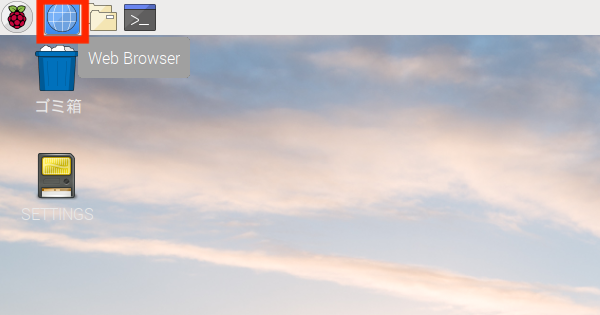
\includegraphics[width=\linewidth]{../../asset/image/textbook-img071.png}
%       1 デスクトップの左上のアイコンを左クリック
%     \end{minipage}
%     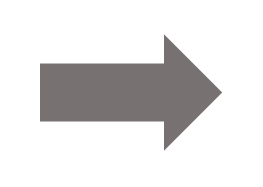
\includegraphics[width=1.505cm]{../../asset/image/textbook-img073.png}
%     \begin{minipage}{0.45\textwidth}
%       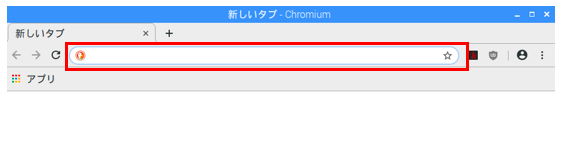
\includegraphics[width=\linewidth]{../../asset/image/textbook-img075.png}
%       2 ブラウザが立ち上がり、赤で囲われている部分を左クリック
%     \end{minipage}
%   \end{minipage}

%   \hfill\begin{minipage}{0.45\textwidth}
%     {\centering
%       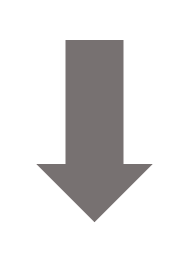
\includegraphics[width=1.707cm]{../../asset/image/textbook-img074.png}
%     }\\
%     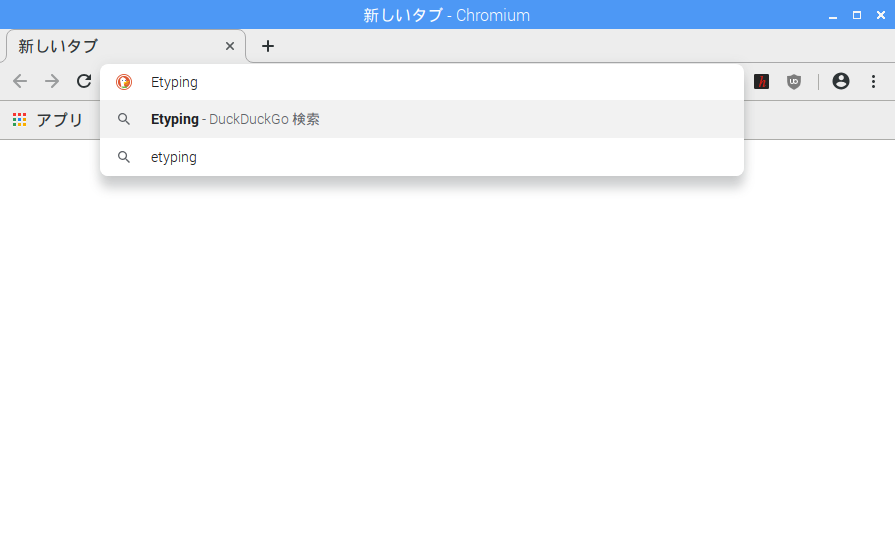
\includegraphics[width=\linewidth]{../../asset/image/textbook-img072.png}
%     3 キーボードでけんさくしたいワードを入力しよう。入力し終えたらenterキーを\ruby{押}{お}そう
%   \end{minipage}

%   \vspace{70mm}

% \end{figure}
% \clearpage


% \begin{figure}
%   \subsubsection{図~\ref{fig:20}のように赤い四角で囲われているところにけんさくしたい言葉を入れてエンターキーを\ruby{押}{お}すとけんさくができます。例えば”ねこ”とけんさくしてみましょう。}
%   \centering
%   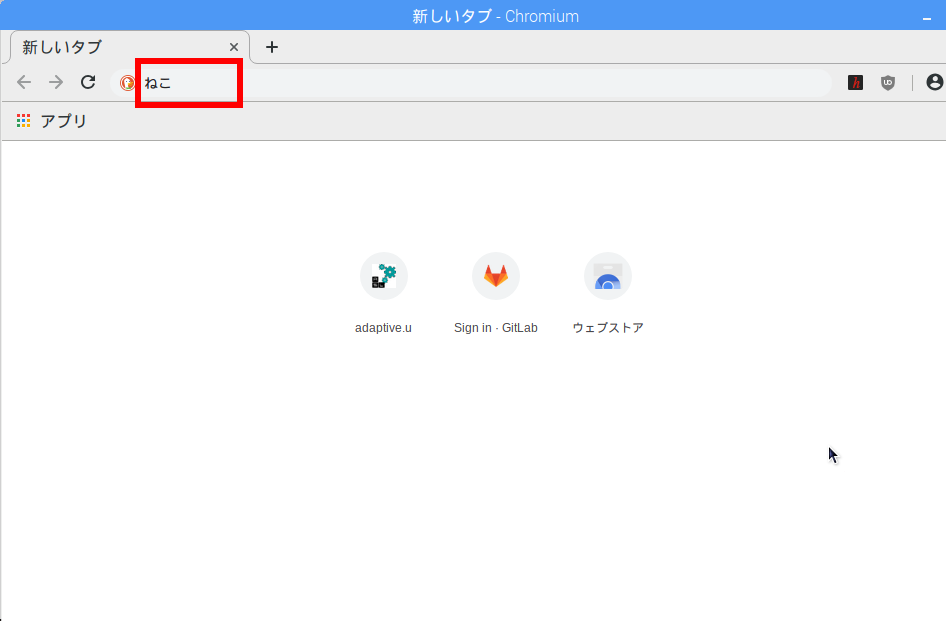
\includegraphics[width=0.45\textwidth]{../../asset/image/textbook-img077.png}
%   \caption{けんさくバー}\label{fig:20}
  
%   \flushleft
%   けんさくすると図~\ref{fig:21}このような感じになります。青線で囲んであるところは今けんさくした言葉です。赤線で囲われている\textbf{\ruby{画像}{がぞう}}をクリックすると\ruby{画像}{がぞう}をけんさくできます。クリックしてみましょう。


%   \centering
%   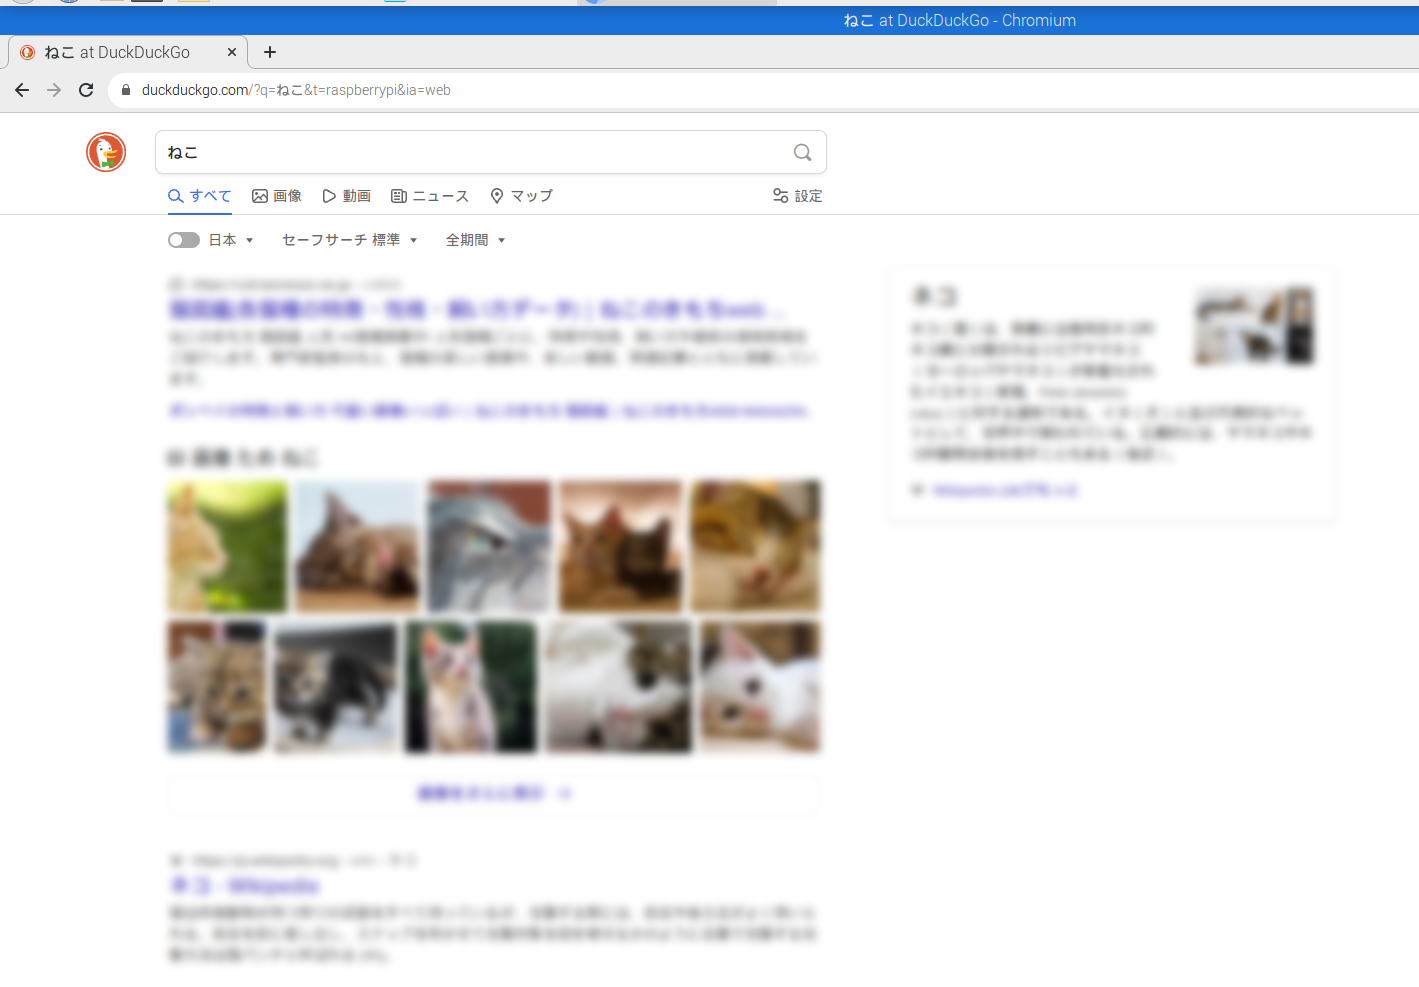
\includegraphics[width=0.45\textwidth]{../../asset/image/textbook-img078.png}
%   \caption{”ねこ”けんさく結果\\
%   けんりの関けいで\ruby{画像}{がぞう}をぼかしてあります}\label{fig:21}
%   \flushleft
%   図~\ref{fig:22}のように”ねこ”の\ruby{画像}{がぞう}がたくさんでてきました。
%   \textbf{すべて}をクリックすると先ほどの~\ref{fig:20}のようなホームページけんさくに\ruby{戻}{もど}れます。


%   \centering
%   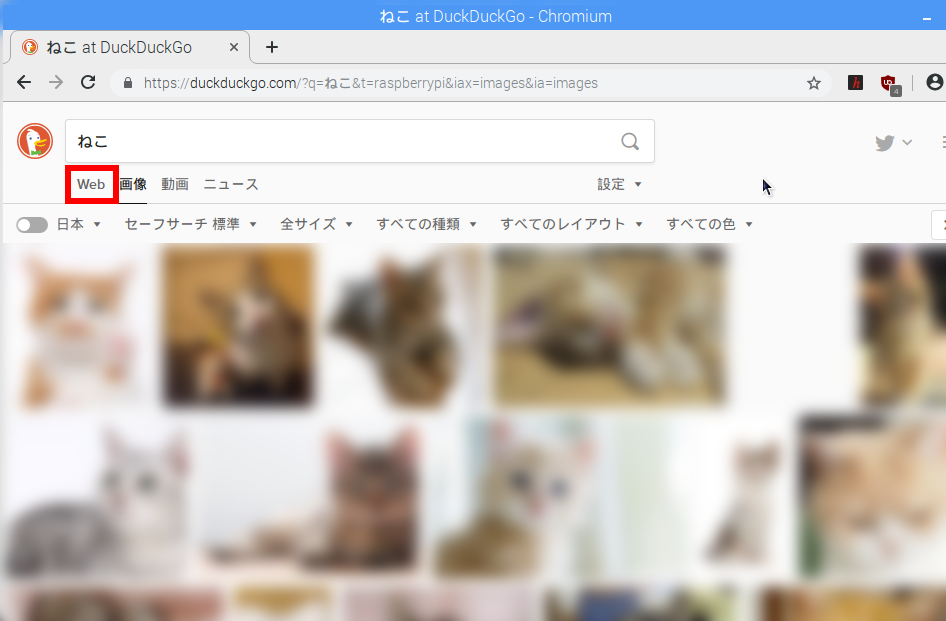
\includegraphics[width=0.45\textwidth]{../../asset/image/textbook-img079.png}
%   \caption{”ねこ”\ruby{画像}{がぞう}けんさく結果}\label{fig:22}
%   \flushleft
%   \noindent \textbf{問題 1-12}\\
%   自分の好きなキーワードをけんさくしてみよう

% \end{figure}
% \clearpage


%
% subsubsection 2
%
\subsubsection{キーボード入力の練習をしよう}
\hrule\vspace*{5mm}

キーボードで文字を入力することをタイピングと言います。
ここでは、タイピング練習ができるウェブサイト「e-typing」を使って、タイピングに\ruby{慣}{な}れましょう。
なお、パソコンで日本語を入力するときは、ローマ字入力が基本ですので、不慣れな場合は、
下のローマ字・アルファベット表で入力方法を確認してください。

\begin{figure}[hb]
  \centering
    % 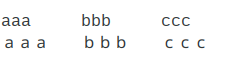
\includegraphics[keepaspectratio, height=20mm]{../../asset/image/textbook-img066.png}
    % 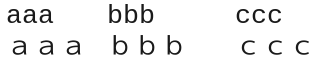
\includegraphics[keepaspectratio, width=0.5\columnwidth]{../../asset/image/textfig_005.png}
    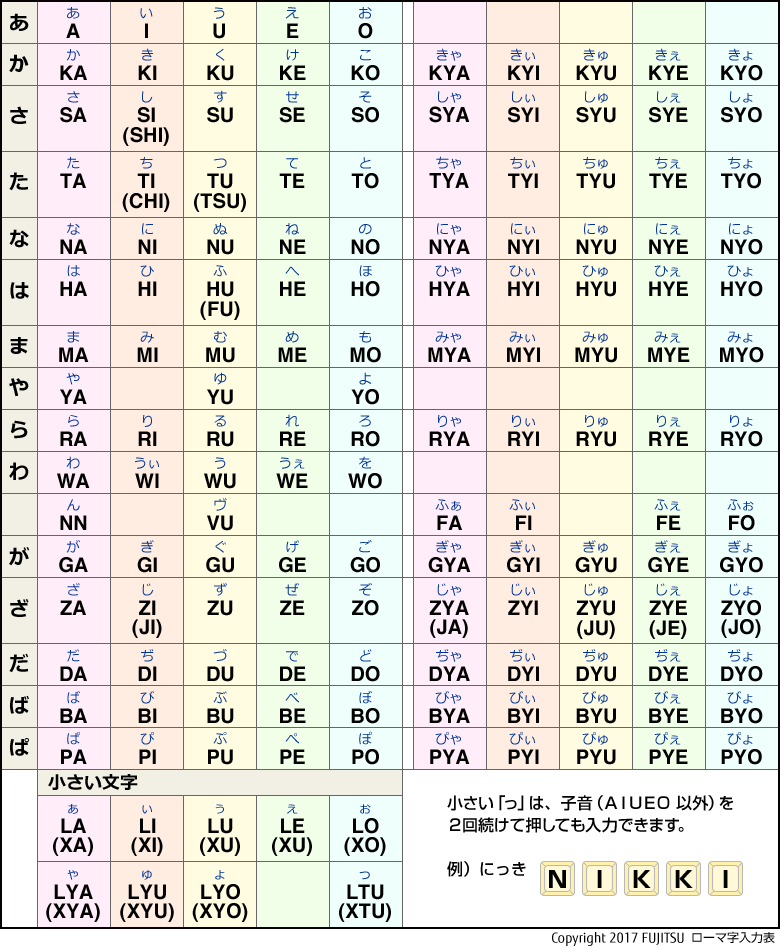
\includegraphics[scale=0.4]{../../asset/image/textbook-img080.png}
    \caption{ローマ字・アルファベット表}
    \label{fig:22}
\end{figure}

{\bf タイピング練習の手順}

\begin{minipage}[t]{0.49\columnwidth}
  \textcircled{\scriptsize{1}}\\
  ブラウザで「etyping」を\ruby{検索}{けんさく}して、タイピング練習ができるウェブサイト
  「e-typing」をみつけましょう（右図のように\ruby{検索}{けんさく}できたら、
  赤わくのリンクをクリックしてください）
\end{minipage}\hfill
%
\begin{minipage}[t]{0.49\columnwidth}
  \centering
  \vbox to 0pt{\vskip-3mm
    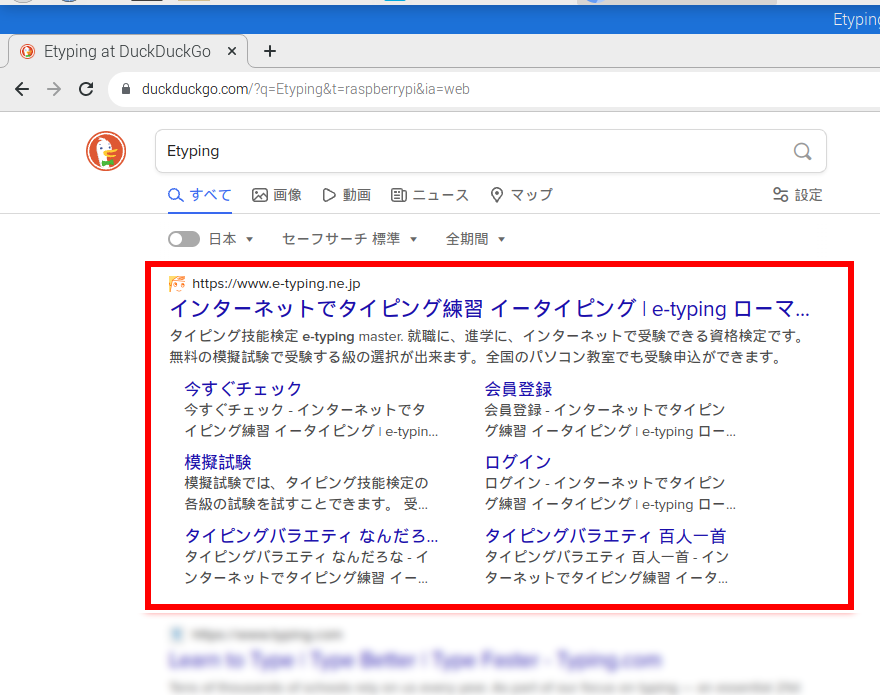
\includegraphics[scale=0.3]{../../asset/image/textbook-img086x.png}
  \vss}
  \vspace{35mm}
\end{minipage}

\begin{minipage}[t]{0.49\columnwidth}
  \textcircled{\scriptsize{2}}\\
  右図のようにホームページが開けたら、「今すぐチェック！」ボタンをクリックしましょう
\end{minipage}\hfill
%
\begin{minipage}[t]{0.49\columnwidth}
  \centering
  \vbox to 0pt{\vskip-3mm
    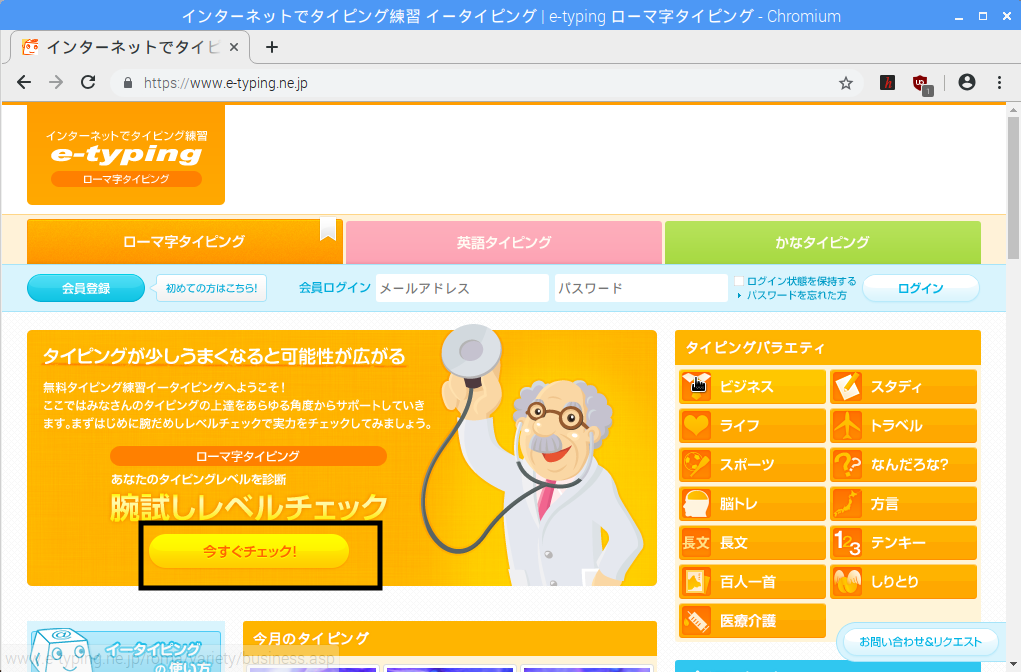
\includegraphics[scale=0.27]{../../asset/image/textbook-img087.png}
  \vss}
  \vspace{50mm}
\end{minipage}

\begin{minipage}[t]{0.49\columnwidth}
  \textcircled{\scriptsize{3}}\\
  もう一度「今すぐチェック！」ボタンをクリックすると、右図のような
  \ruby{腕試}{うでだめ}しレベルチェックウィンドウが表示されますので、
  スタートボタンをクリックします
\end{minipage}\hfill
%
\begin{minipage}[t]{0.49\columnwidth}
  \centering
  \vbox to 0pt{\vskip-3mm
    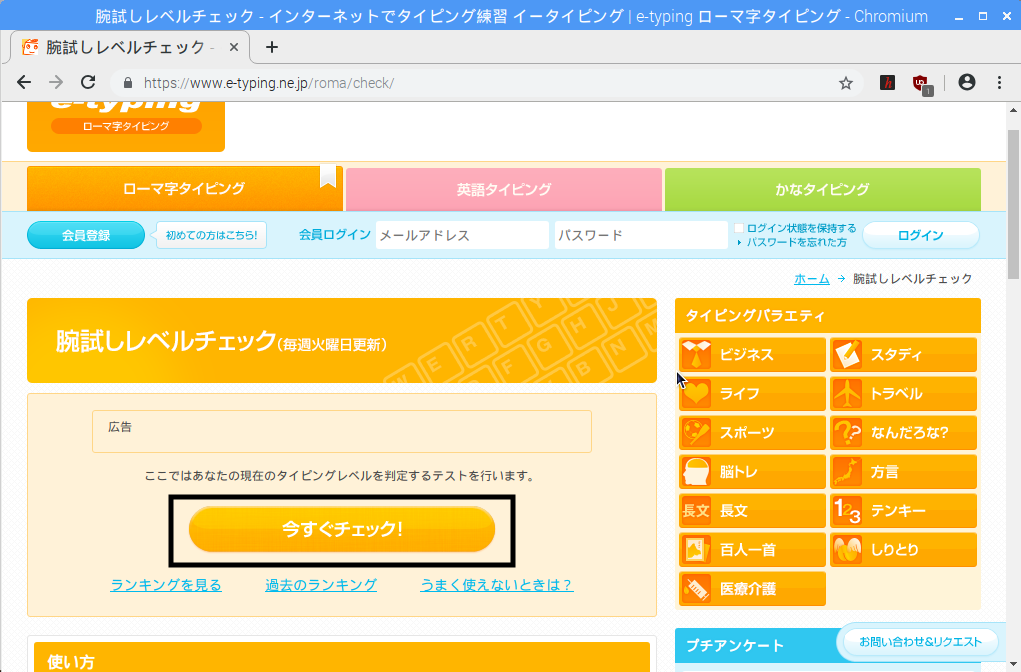
\includegraphics[scale=0.27]{../../asset/image/textbook-img088.png}
  \vss}
  \vspace{50mm}
\end{minipage}

\begin{minipage}[t]{0.49\columnwidth}
  \textcircled{\scriptsize{4}}\\
  キーボードのスペースキーを押すとゲームがスタートします
\end{minipage}\hfill
%
\begin{minipage}[t]{0.49\columnwidth}
  \centering
  \vbox to 0pt{\vskip-3mm
    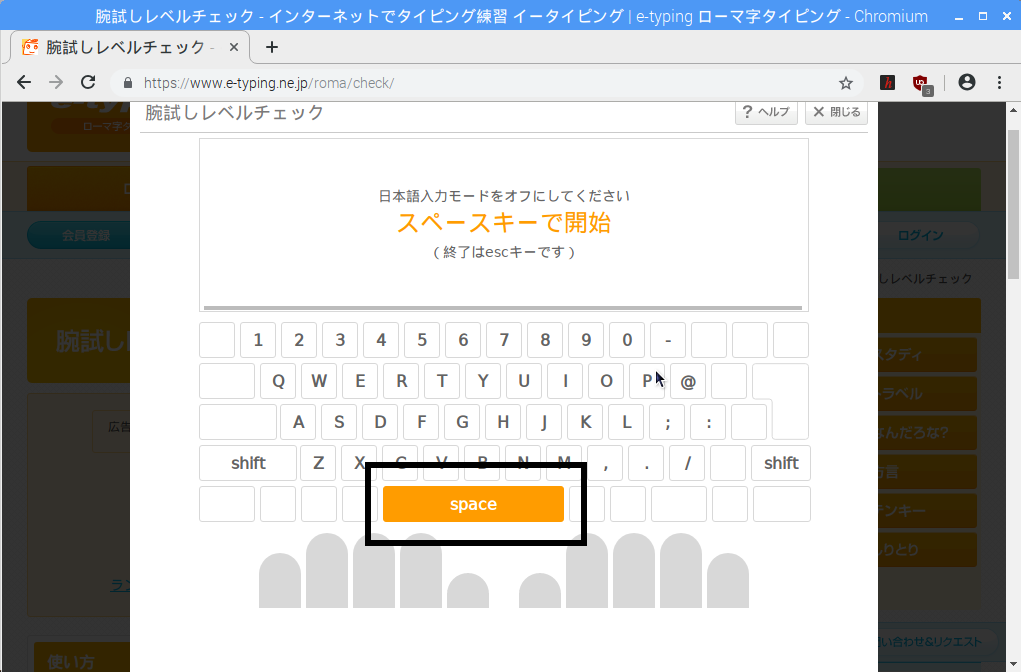
\includegraphics[scale=0.27]{../../asset/image/textbook-img090.png}
  \vss}
  \vspace{50mm}
\end{minipage}

\begin{minipage}[t]{0.49\columnwidth}
  \textcircled{\scriptsize{5}}\\
  ゲームでは、画面左上の文字をキーボードで入力します\\
  キーの位置は画面中央のキーボードにオレンジ色で表示されます\\
  \ruby{慣}{な}れてきたら、画面下のオレンジ色の指で、オレンジ色のキーを\ruby{押}{お}せるように練習してみましょう
\end{minipage}\hfill
%
\begin{minipage}[t]{0.49\columnwidth}
  \centering
  \vbox to 0pt{\vskip-3mm
    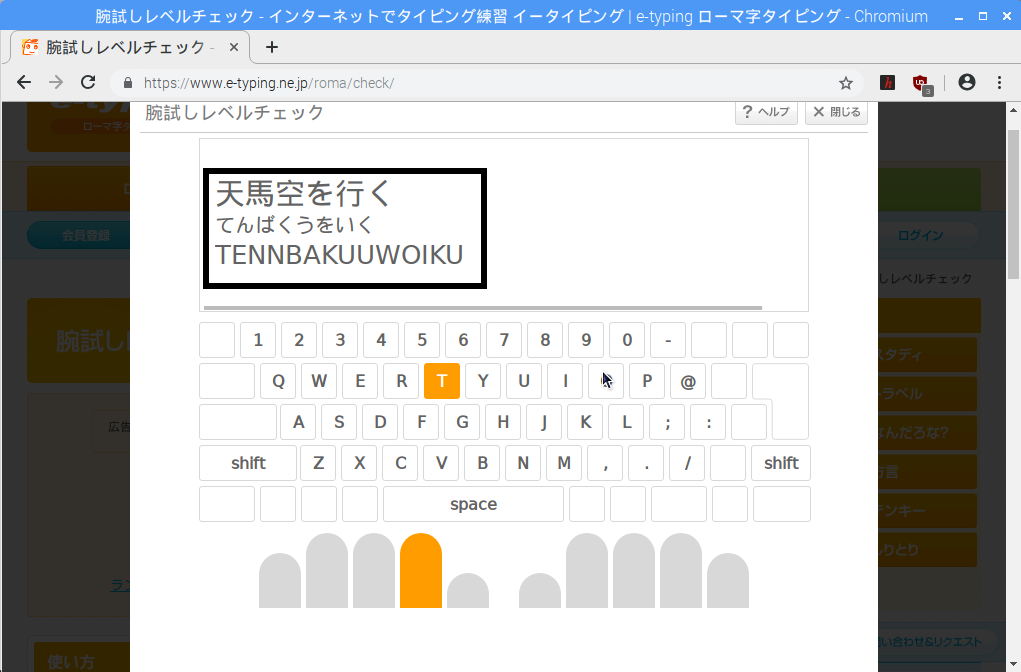
\includegraphics[scale=0.27]{../../asset/image/textbook-img089.png}
  \vss}
  \vspace{50mm}
\end{minipage}



% \begin{figure}[t]
%   \subsection{例題 1-12 キーボード入力の練習をしよう}
%   ブラウザで”Etyping”とけんさくし、キーボードタイピングサイトでタイピングに\ruby{慣}{な}れよう

%   \textbf{考え方}\\
%   \textbf{タイピング} ・・・キーボードで文字を入力すること
%   \vskip.5\baselineskip
%   \begin{minipage}{\textwidth}
%     \raisebox{30mm}{
%       \begin{minipage}{0.65\textwidth}
%         パソコンでの文字入力はローマ字入力が\ruby{基本}{きほん}です。
%         けんさくなどをしたいとき、キーボードで文字を入力します。
%         今回はタイピング練習サイト”Etyping”でタイピングを
%         練習しましょう。

%         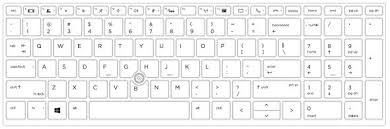
\includegraphics[width=0.7\linewidth]{../../asset/image/textbook-img081.png}
%         
\includegraphics[width=0.25\linewidth]{../../asset/image/textbook-img082.png}
%       \end{minipage} }
%     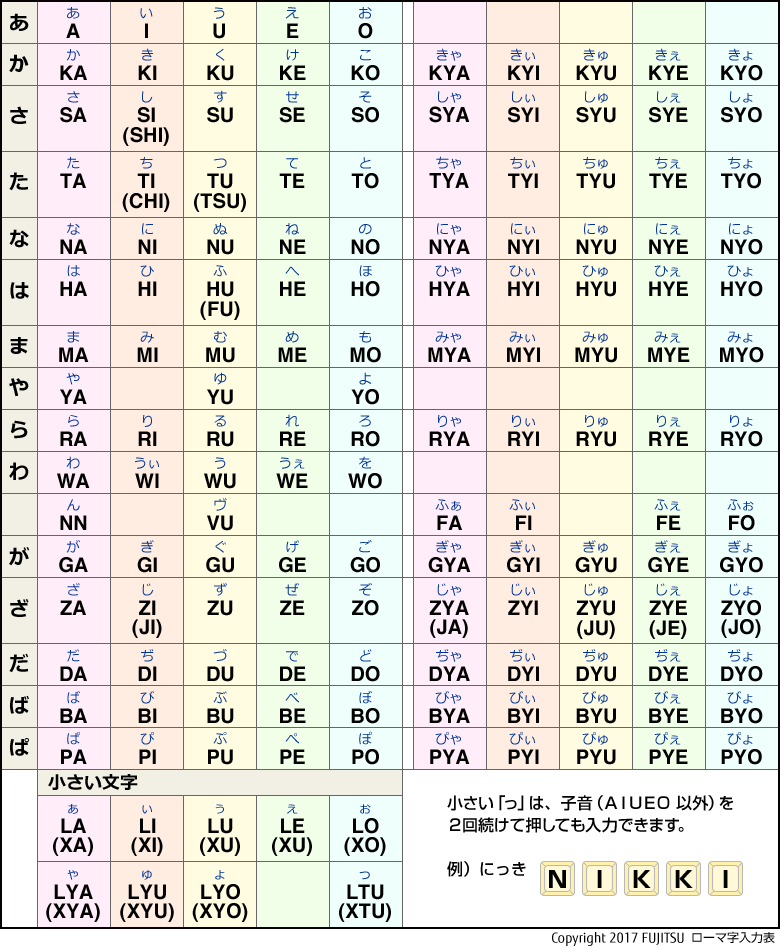
\includegraphics[width=0.3\textwidth]{../../asset/image/textbook-img080.png}
%   \end{minipage}

%   \centering

%   {\centering
%     \textbf{まずはタイピングゲームを開こう}
%     \par}

%   \centering

%   \begin{minipage}{0.4\textwidth}
%     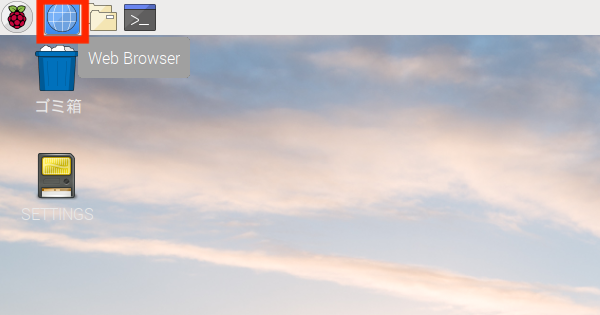
\includegraphics[width=\linewidth]{../../asset/image/textbook-img071.png}
%     1 左上のアイコンをクリックしよう
%   \end{minipage}
%   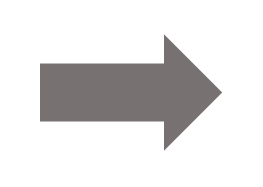
\includegraphics[width=2cm]{../../asset/image/textbook-img084.png}
%   \begin{minipage}{0.4\textwidth}
%     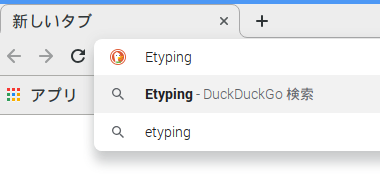
\includegraphics[width=\linewidth]{../../asset/image/textbook-img083.png}
%     2 けんさくらんに”Etyping”と入力しenterを\ruby{押}{お}そう
%   \end{minipage}
%   \vskip.5\baselineskip
%   \begin{minipage}{0.45\textwidth}
%     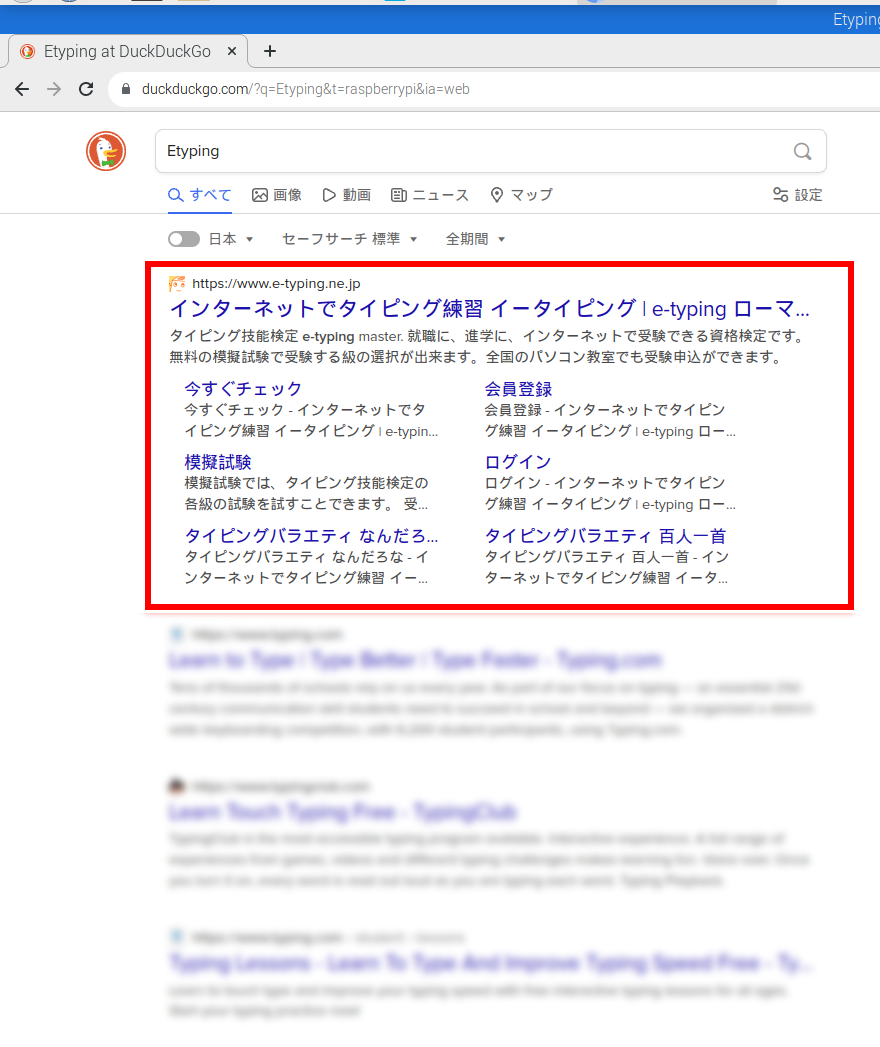
\includegraphics[width=\linewidth]{../../asset/image/textbook-img086.png}
%     3 サイトに入りましょう。赤わくで囲われているところのうち、一番上の「インターネットでタイピング練習 イータイピング」をクリックします。
%   \end{minipage}
%   \begin{minipage}{0.45\textwidth}
%     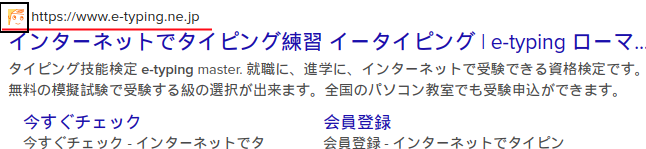
\includegraphics[width=\linewidth]{../../asset/image/textbook-img085.png}
%     赤線で線が引かれているところ、黒い四角で囲んであるアイコンをよく確かめてください。
%   \end{minipage}

%   \centering

% \end{figure}

% \clearpage

% \begin{figure}
%   \textbf{考え方(続き)}

%   \centering
%   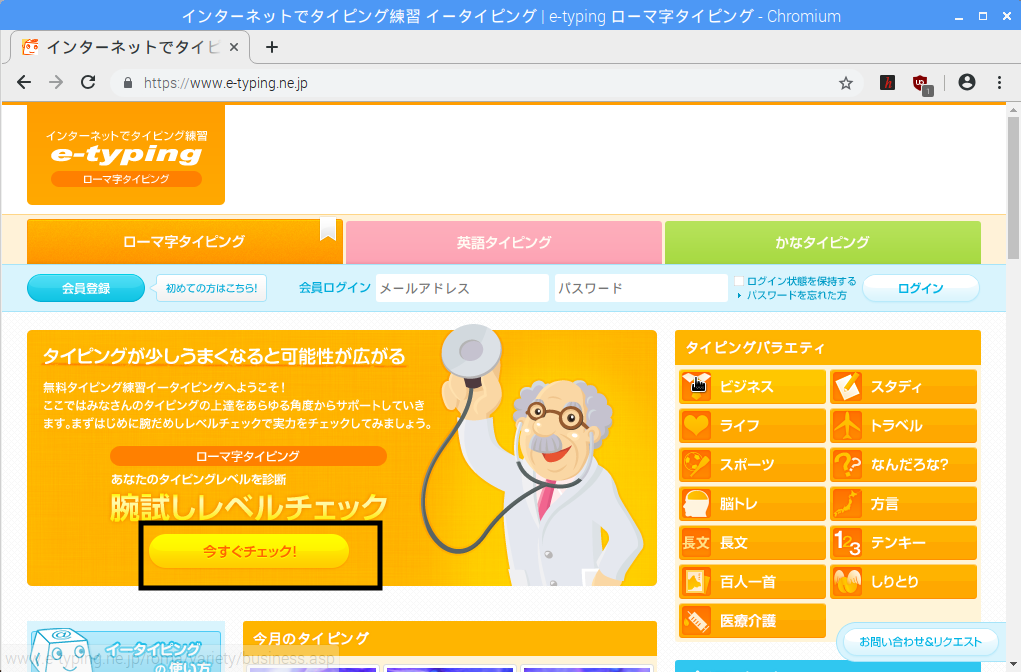
\includegraphics[width=0.7\textwidth]{../../asset/image/textbook-img087.png}
%   \begin{minipage}{0.7\textwidth}
%     4 ホームページが開けたら黒で囲んである\textbf{今すぐチェック!}をクリックしよう

%   \end{minipage}
% \end{figure}





% \begin{figure}
%   \centering
%   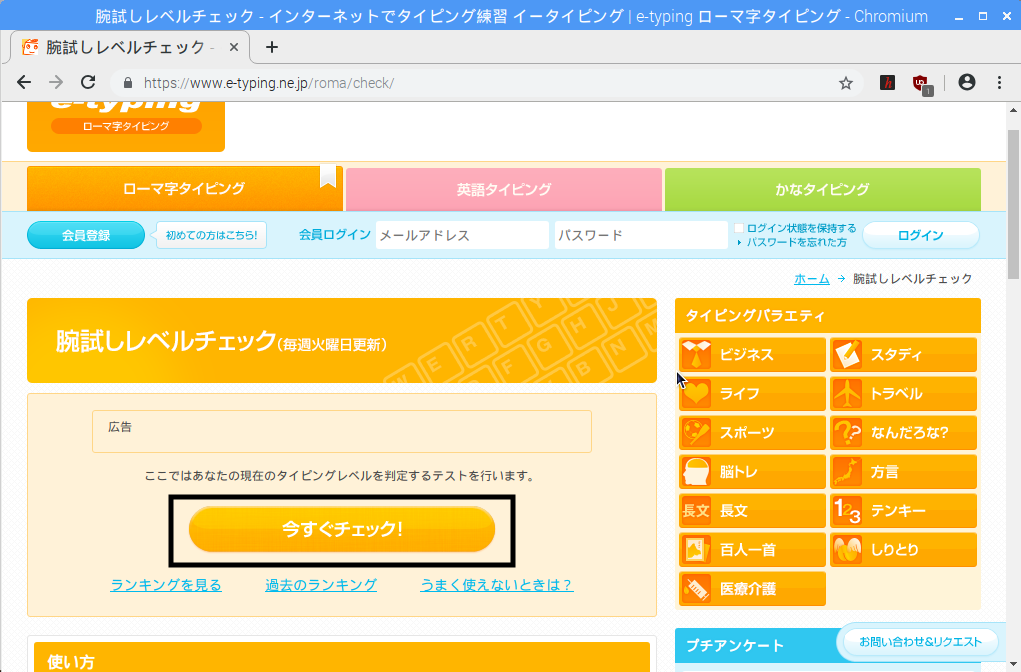
\includegraphics[width=0.7\textwidth]{../../asset/image/textbook-img088.png}

%   \begin{minipage}{0.7\textwidth}
%     5 黒い四角で囲んである\textbf{今すぐチェック!}をもう一度クリックします。
%   \end{minipage}
% \end{figure}

% \clearpage



% \begin{figure}[t]
%   \subsection{ 考え方（続き）}

%   \centering
%   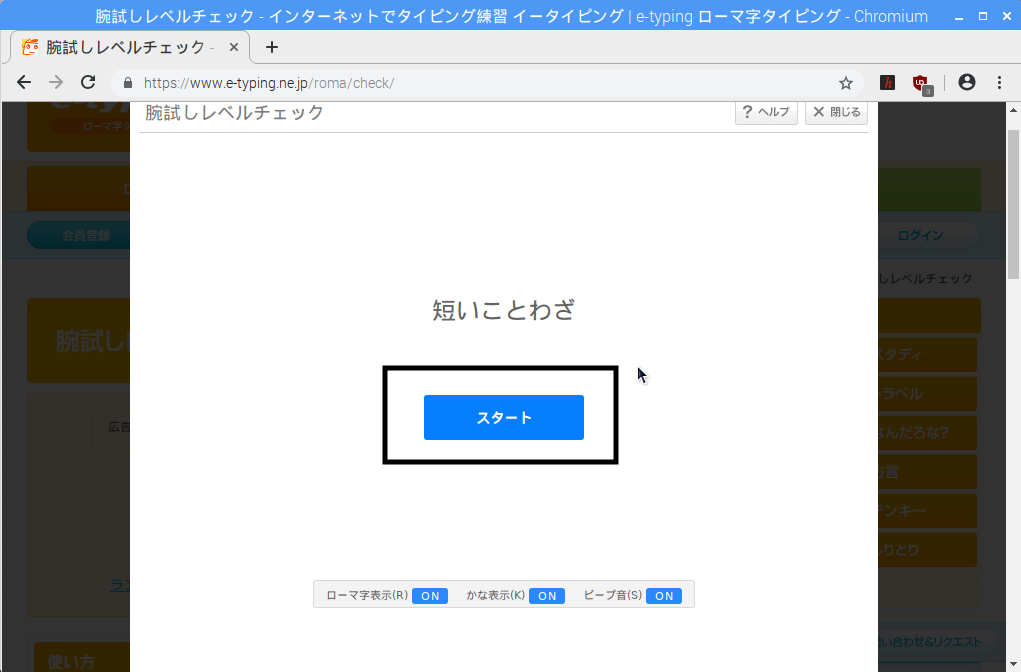
\includegraphics[width=	0.6\textwidth]{../../asset/image/textbook-img091.png}
%   \raisebox{40mm}{\begin{minipage}{5cm}
%       6 黒い四角で囲んである
%       \textbf{スタート}を
%       クリックします。
%     \end{minipage}
%   }

%   \bigskip
%   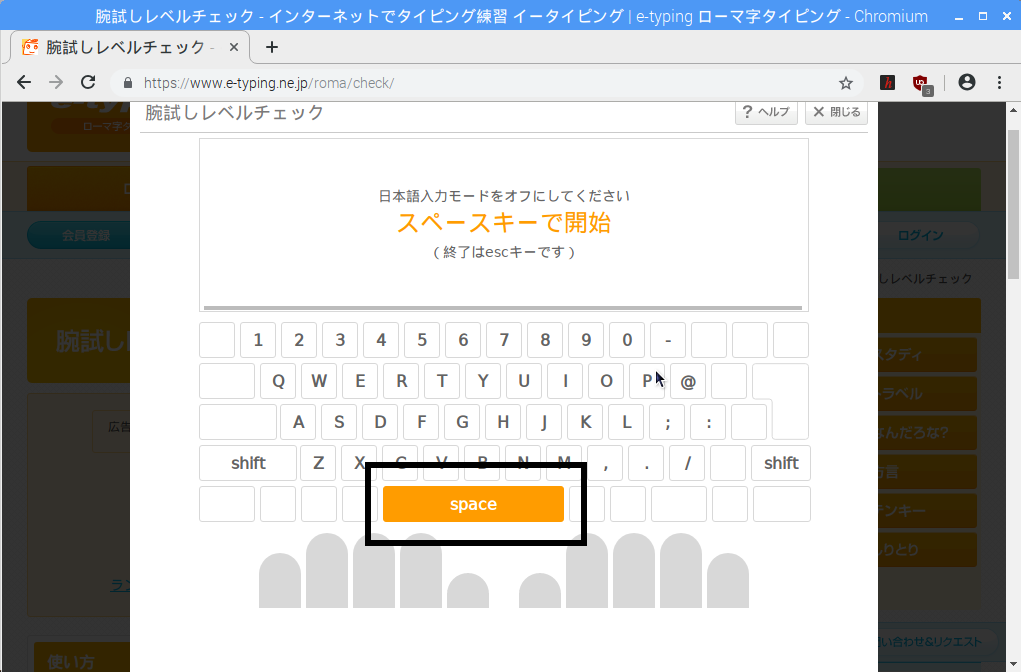
\includegraphics[width=0.6\textwidth]{../../asset/image/textbook-img090.png}
%   \raisebox{40mm}{\begin{minipage}{5cm}
%       7 キーボードのスペースキーを\ruby{押}{お}すとゲームがスタートします。


%       \bigskip
%     \end{minipage}
%   }

%   \bigskip


%   \bigskip

%   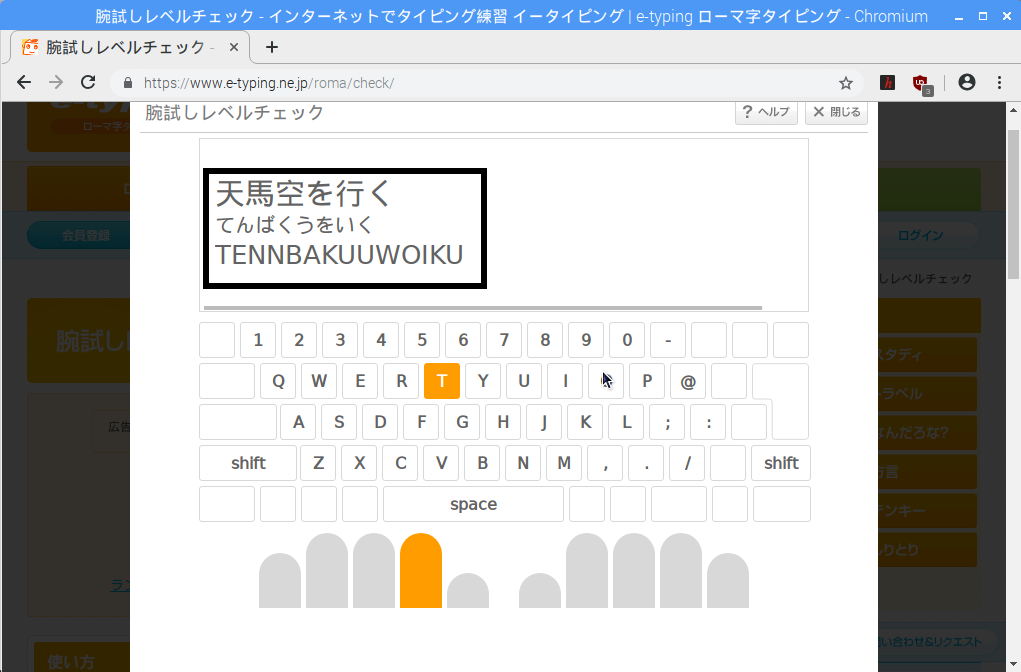
\includegraphics[width=0.6\textwidth]{../../asset/image/textbook-img089.png}
%   \raisebox{30mm}{\begin{minipage}{5cm}
%       8 ゲームでは黒で囲んである文字をキーボードで入力します。


%       \bigskip

%       キーの位置は画面にオレンジで色がついています。


%       \bigskip

%       \ruby{慣}{な}れてきたら、オレンジになっている指でキーボードを\ruby{押}{お}せるように練習してみましょう。


%       \bigskip
%     \end{minipage}
%   }

%   \bigskip
%   \bigskip
%   \bigskip
%   \bigskip
% \end{figure}

\clearpage

%
% subsection 1.3
%
\subsection{画面の見た目を自分の好みに変えよう}

ここでは、ラズパイのデスクトップに表示される画像（かべ紙）やウィンドウの色などを変えてみましょう。

%
% subsubsection 1
%
\subsubsection{画像を\ruby{検索}{けんさく}して、目当ての画像を保存しよう}
\hrule\vspace*{5mm}

ブラウザで\ruby{検索}{けんさく}した\ruby{画像}{がぞう}は、ラズパイのフォルダ内に\ruby{保存}{ほぞん}することができます。
フォルダ名は、中に入っている\ruby{画像}{がぞう}やファイルに関連する名前にすると、
どんな\ruby{画像}{がぞう}やファイルが\ruby{保存}{ほぞん}されているか分かりやすくなります。
ここでは、\texttt{Pictures}フォルダの中に\texttt{usagi}フォルダを作成して、
その中に\ruby{画像検索}{がぞうけんさく}で見つけたうさぎの\ruby{画像}{がぞう}を\ruby{保存}{ほぞん}しましょう。\\

{\bf 手順}

\begin{minipage}[t]{0.49\columnwidth}
  \textcircled{\scriptsize{1}}\\
  ファイルマネージャを使って、\texttt{Pictures}フォルダの中に\texttt{usagi}フォルダを作成しましょう。
\end{minipage}\hfill
%
\begin{minipage}[t]{0.49\columnwidth}
  \centering
  \vbox to 0pt{\vskip-3mm
    % 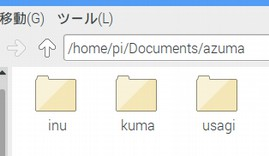
\includegraphics[scale=0.3]{../../asset/image/textbook-img094.jpg}
    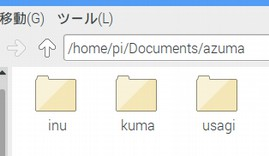
\includegraphics[width=0.5\linewidth]{../../asset/image/textbook-img094.jpg}
  \vss}
  \vspace{45mm}
\end{minipage}

\begin{minipage}[t]{0.49\columnwidth}
  \textcircled{\scriptsize{2}}\\
  ブラウザを使って「うさぎ」の\ruby{画像}{がぞう}を\ruby{検索}{けんさく}しましょう。
  目当ての画像を見つけたらクリックして大きく表示します
\end{minipage}\hfill
%
\begin{minipage}[t]{0.49\columnwidth}
  \centering
  \vbox to 0pt{\vskip-3mm
    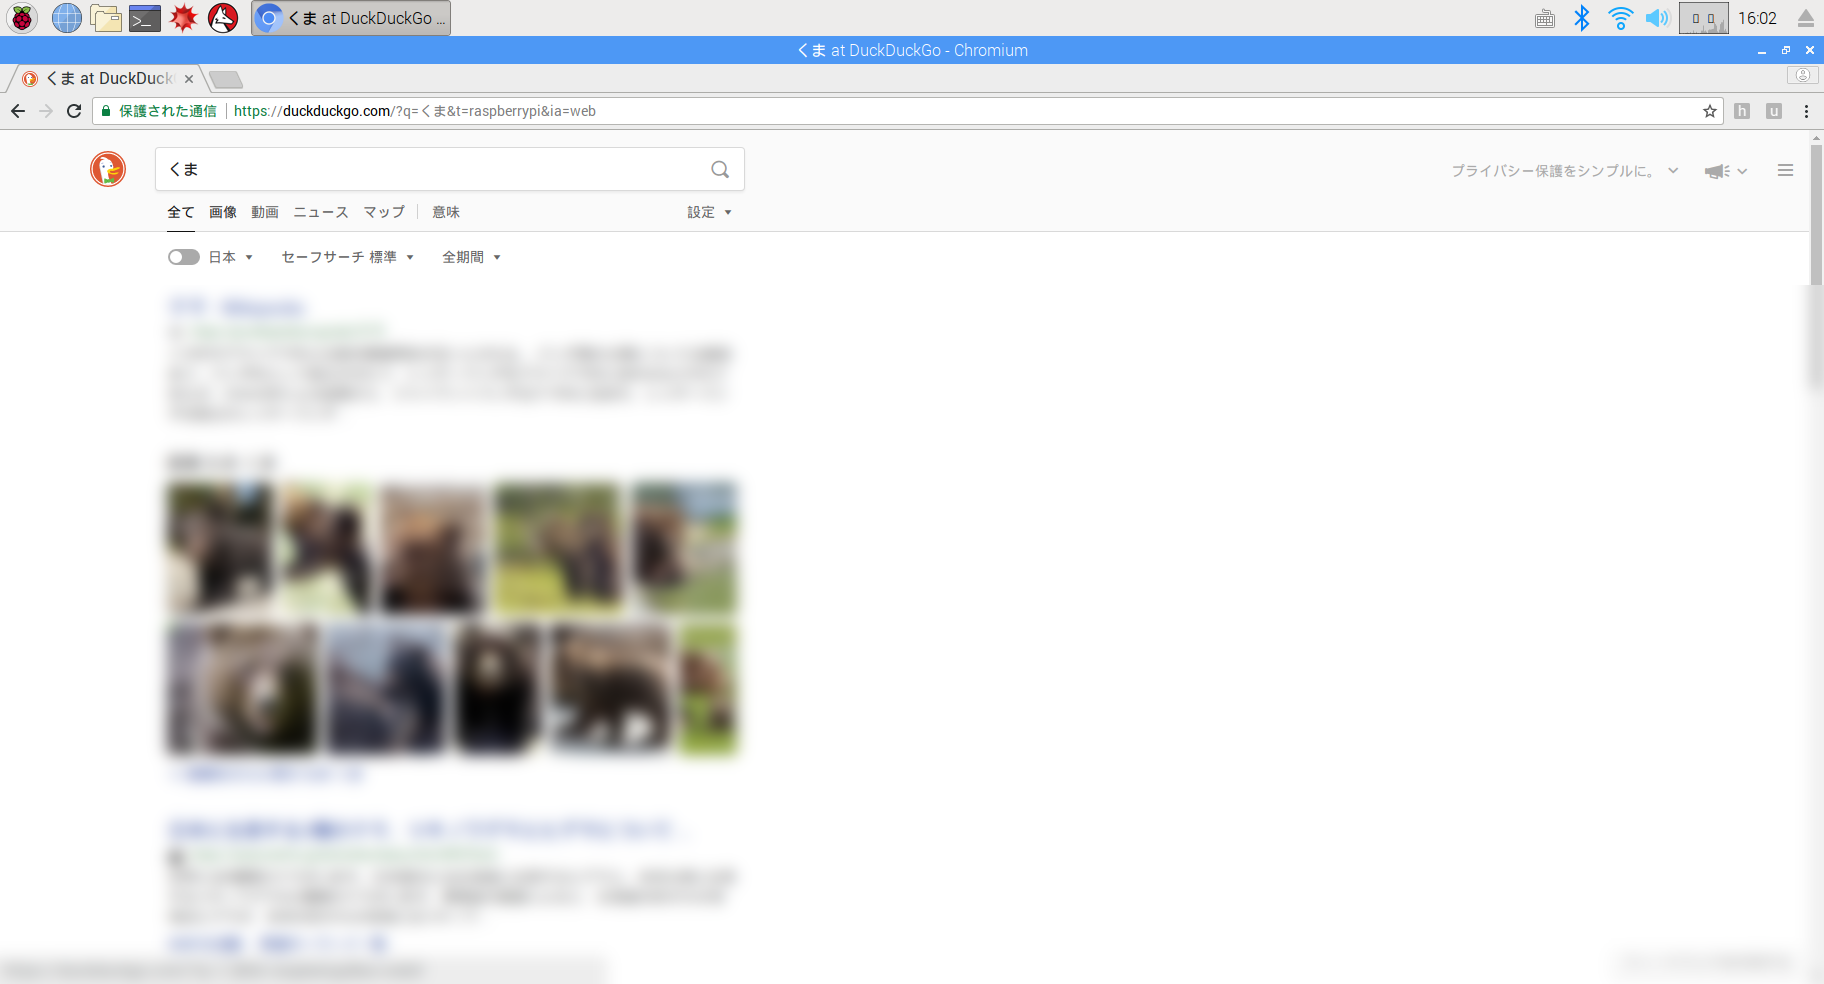
\includegraphics[height=0.5\linewidth]{../../asset/image/textbook-img096.png}
  \vss}
  \vspace{45mm}
\end{minipage}

\begin{minipage}[t]{0.49\columnwidth}
  \textcircled{\scriptsize{3}}\\
  \ruby{画像}{がぞう}の上で右クリックしてメニューを表示し、「名前をつけて画像を保存」をクリックします
\end{minipage}\hfill
%
\begin{minipage}[t]{0.49\columnwidth}
  \centering
  \vbox to 0pt{\vskip-3mm
    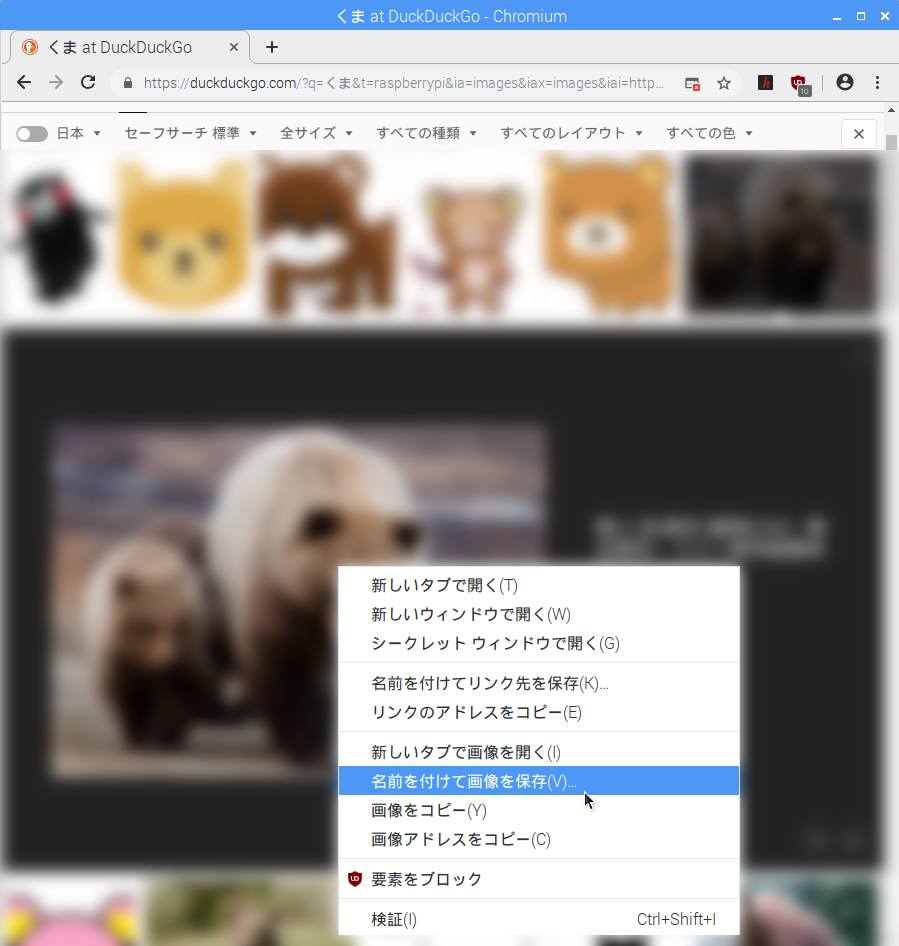
\includegraphics[width=0.5\linewidth]{../../asset/image/textbook-img095.png}
  \vss}
  \vspace{45mm}
\end{minipage}

\begin{minipage}[t]{0.49\columnwidth}
  \textcircled{\scriptsize{4}}\\
  ウィンドウ左側からPicturesフォルダを選択し、\texttt{usagi}フォルダをダブルクリックして保存場所を指定します。
  上のテキストボックスに名前を入力したら、右下の「SAVE」をクリックします
  （この例では画像に\texttt{cute.jpg}という名前を付けています）
\end{minipage}\hfill
%
\begin{minipage}[t]{0.49\columnwidth}
  \centering
  \vbox to 0pt{\vskip-3mm
    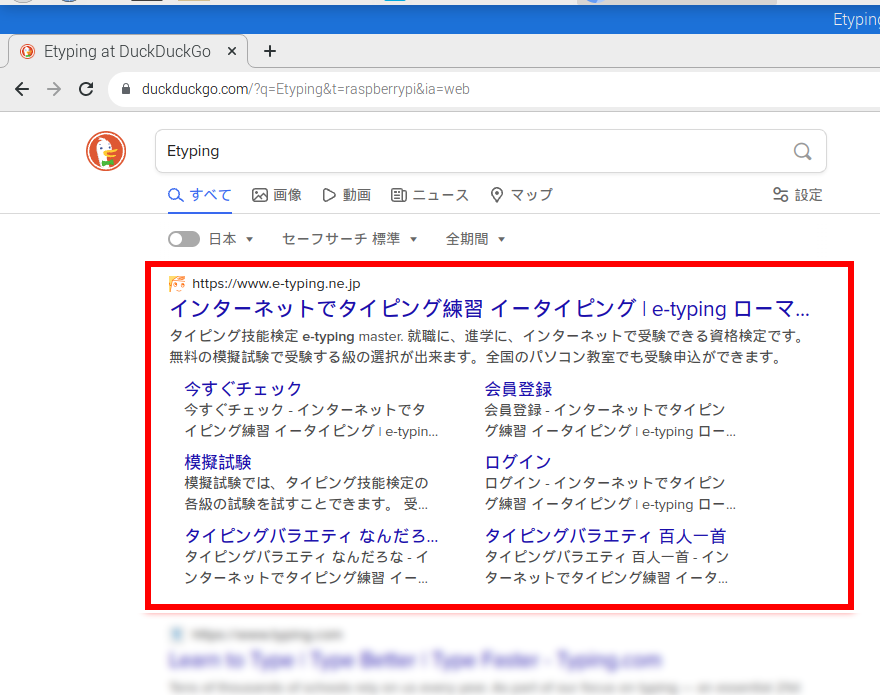
\includegraphics[scale=0.3]{../../asset/image/textbook-img086x.png}
  \vss}
  \vspace{45mm}
\end{minipage}

\begin{minipage}[t]{0.49\columnwidth}
  \textcircled{\scriptsize{5}}\\
  ファイルマネージャでウィンドウ左側からPicturesフォルダを選択し、\texttt{usagi}フォルダをダブルクリックして保存場所を指定します。
  上のテキストボックスに名前を入力したら、右下の「SAVE」をクリックします
  （この例では画像に\texttt{cute.jpg}という名前を付けています）
\end{minipage}\hfill
%
\begin{minipage}[t]{0.49\columnwidth}
  \centering
  \vbox to 0pt{\vskip-3mm
    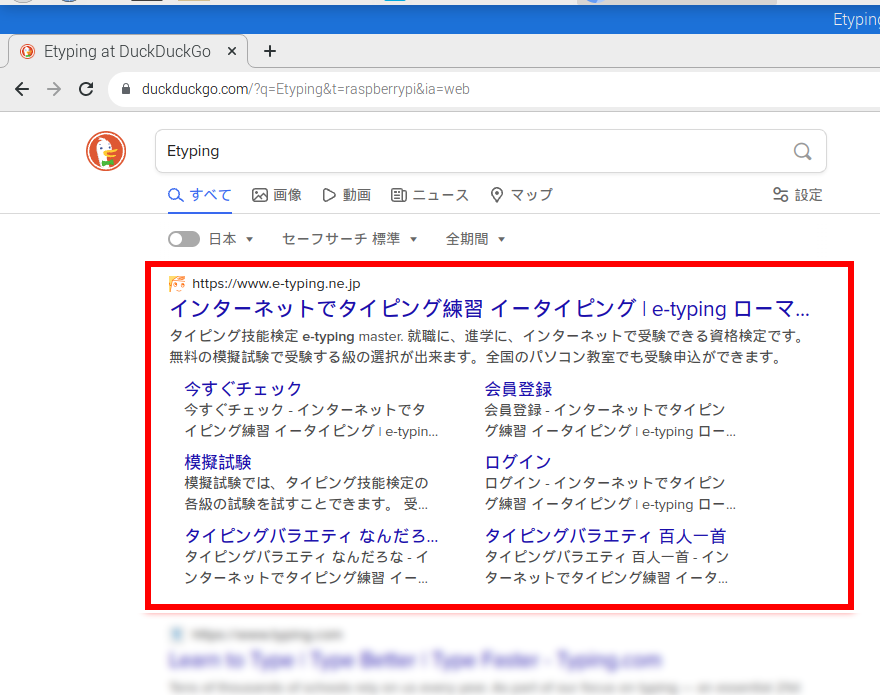
\includegraphics[scale=0.3]{../../asset/image/textbook-img086x.png}
  \vss}
  \vspace{45mm}
\end{minipage}



\begin{figure}[t]
  \subsection{例題 1-13 \ruby{画像}{がぞう}けんさくし、\ruby{画像}{がぞう}を\ruby{保存}{ほぞん}しよう}
  Documentsフォルダに自分の名前のフォルダを作り、さらにその中にkuma、usagi、inuフォルダを作成、そのフォルダに\ruby{画像}{がぞう}けんさくで得たクマ、うさぎ、犬の\ruby{画像}{がぞう}をそれぞれ\ruby{対応}{たいおう}するフォルダに\ruby{保存}{ほぞん}しよう

  \textbf{考え方}

  \bigskip
  \centering

    \begin{minipage}{0.4\textwidth}
      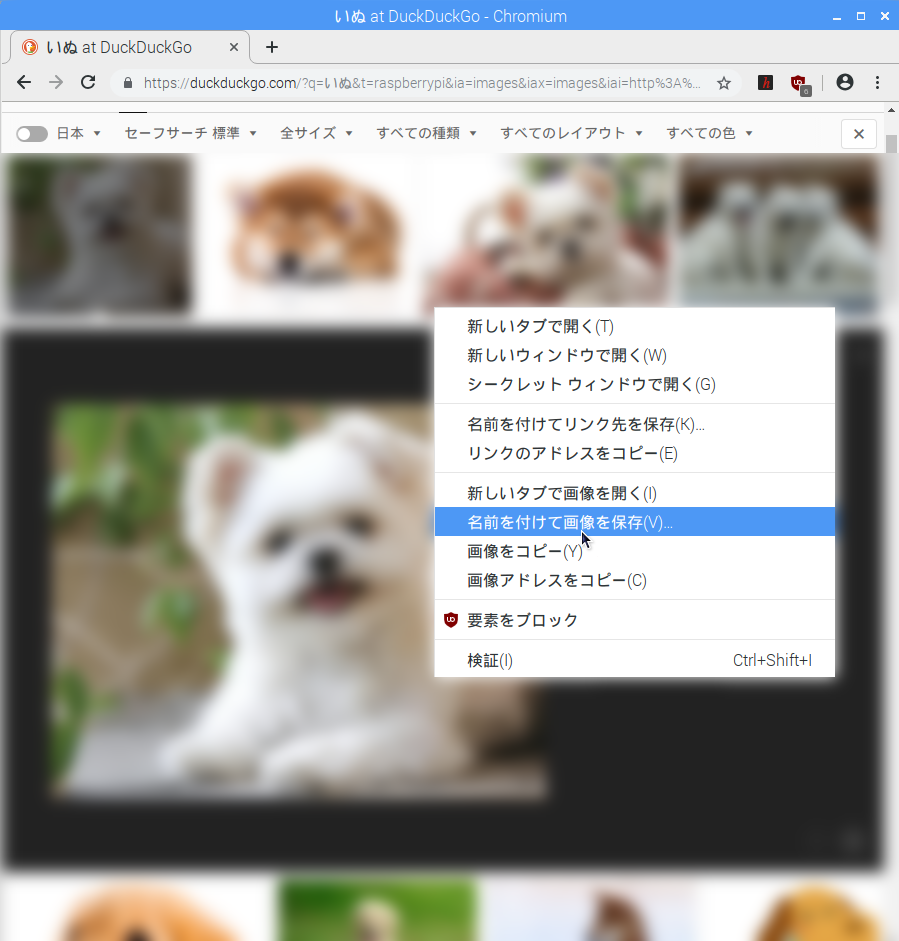
\includegraphics[width=\linewidth]{../../asset/image/textbook-img092.png}
    \end{minipage}
    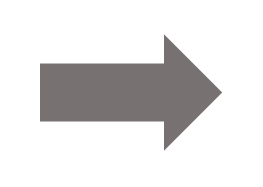
\includegraphics[width=2cm]{../../asset/image/textbook-img073.png}
    \begin{minipage}{0.4\textwidth}
      
\includegraphics[width=0.5\linewidth]{../../asset/image/textbook-img044.png}
    \end{minipage}

  \flushleft
  {\bfseries
    フォルダに\ruby{画像}{がぞう}を\ruby{保存}{ほぞん}しよう}

  ブラウザの\ruby{画像}{がぞう}けんさくしたいものはラズベリーパイのフォルダ内に\ruby{保存}{ほぞん}することができる

  \ruby{画像}{がぞう}と関連のあるフォルダ名にしておくと、どのような\ruby{画像}{がぞう}が\ruby{保存}{ほぞん}されているのかわかりやすいよ

  \begin{minipage}{0.4\textwidth}
    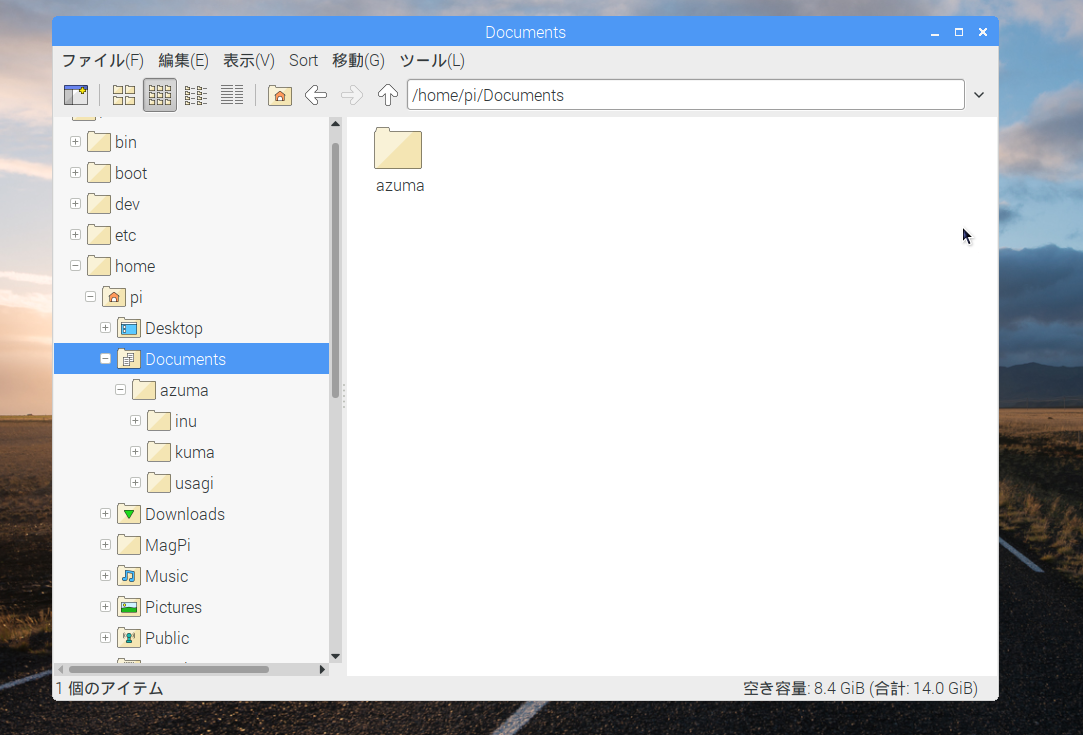
\includegraphics[width=\linewidth]{../../asset/image/textbook-img093.png}
    \flushleft
    1 例題の方法で自分の名前のフォルダをDocuments内に作成しよう
  \end{minipage}
  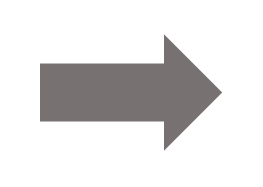
\includegraphics[width=2cm]{../../asset/image/textbook-img073.png}
  \begin{minipage}{0.4\textwidth}
    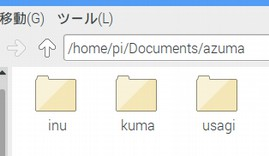
\includegraphics[width=\linewidth]{../../asset/image/textbook-img094.jpg}
    \flushleft
    2 自分のフォルダをダブルクリックし、その中に上の\ruby{画像}{がぞう}のように３つのフォルダを作成
  \end{minipage}

  \begin{minipage}{0.4\textwidth}
    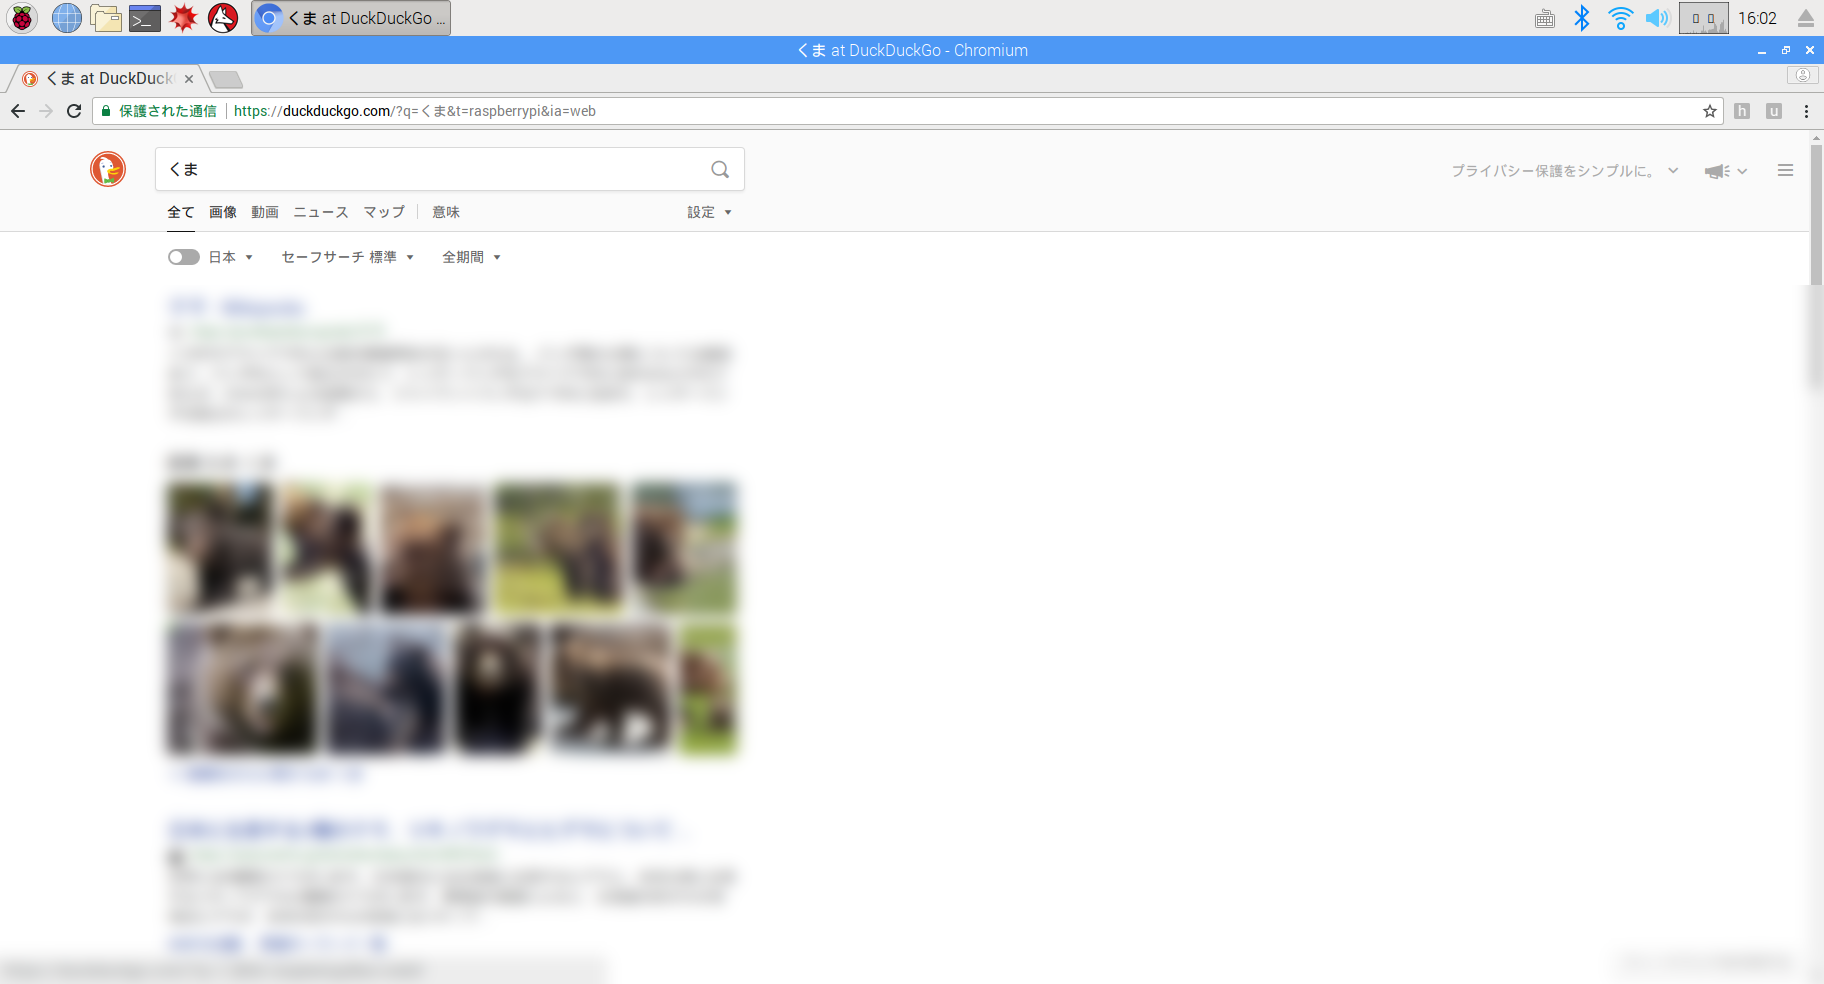
\includegraphics[width=\linewidth]{../../asset/image/textbook-img096.png}
    \flushleft
    3 ブラウザを立ち上げてくまをけんさくし、上の\ruby{画像}{がぞう}の赤色で囲われた”\ruby{画像}{がぞう}”をクリック
  \end{minipage}
  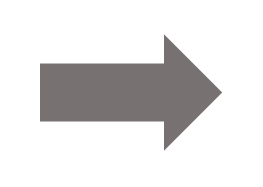
\includegraphics[width=2cm]{../../asset/image/textbook-img073.png}
  \begin{minipage}{0.4\textwidth}
    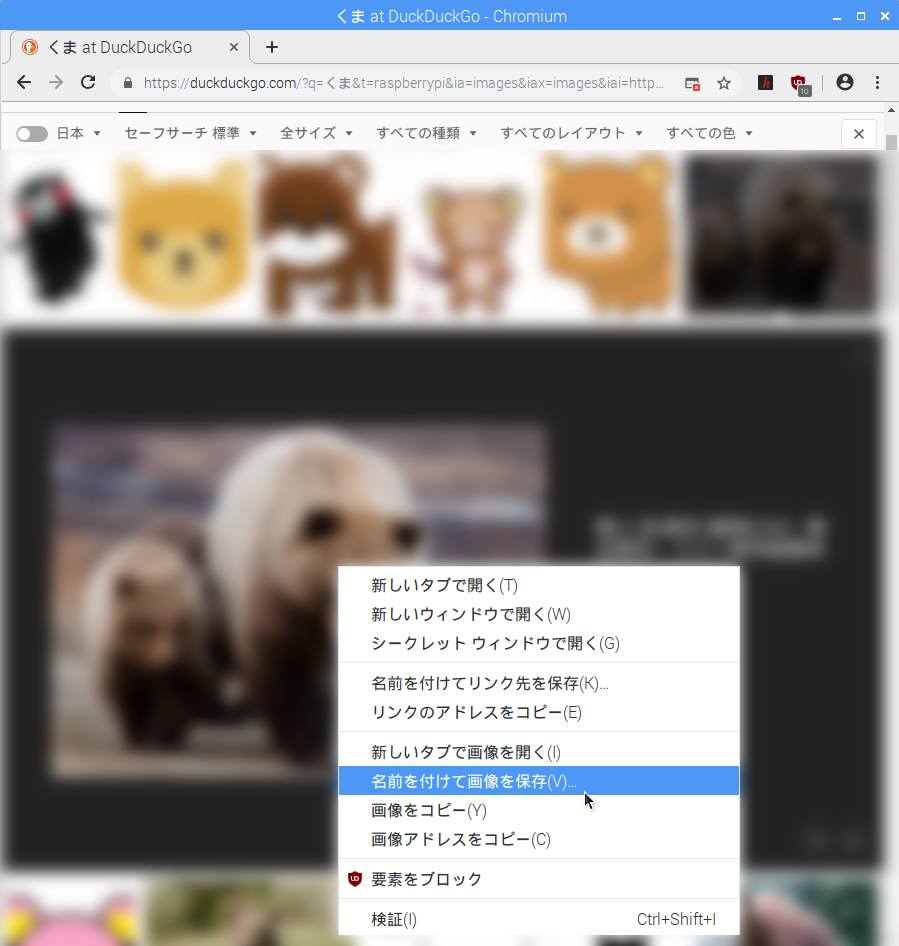
\includegraphics[width=\linewidth]{../../asset/image/textbook-img095.png}
    \flushleft
    4 \ruby{画像}{がぞう}けんさくで好きな\ruby{画像}{がぞう}上で右クリックをし”名前をつけて\ruby{保存}{ほぞん}”をクリック
  \end{minipage}

\end{figure}

\clearpage

\begin{figure}[t]
  \flushleft
  \textbf{考え方（続き）}

  \centering

  \begin{minipage}{0.4\textwidth}
    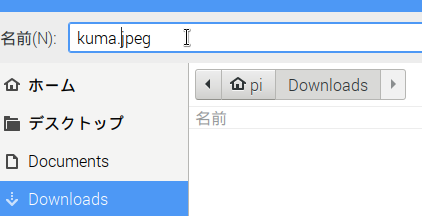
\includegraphics[width=\linewidth]{../../asset/image/textbook-img097.png}
    \flushleft
    5 \ 名前を\ruby{変更}{へんこう}
  \end{minipage}
  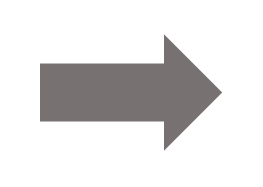
\includegraphics[width=2cm]{../../asset/image/textbook-img073.png}
  \begin{minipage}{0.4\textwidth}
    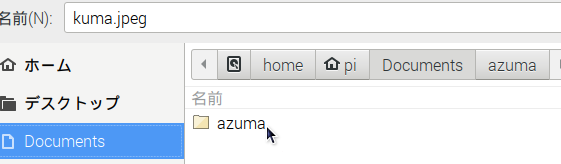
\includegraphics[width=\linewidth]{../../asset/image/textbook-img098.png}
    \flushleft
    6 \ 自分の名前フォルダをダブルクリック
  \end{minipage}

  \bigskip

  \begin{minipage}{0.4\textwidth}
    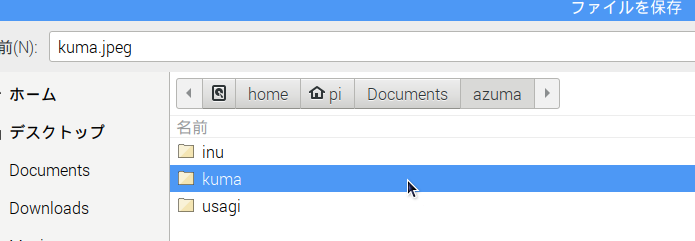
\includegraphics[width=\linewidth]{../../asset/image/textbook-img100.png}
    \flushleft
    7 \ “kuma”フォルダをダブルクリック
  \end{minipage}
  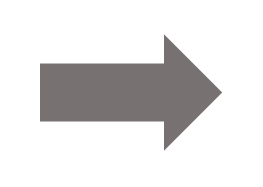
\includegraphics[width=2cm]{../../asset/image/textbook-img073.png}
  \begin{minipage}{0.4\textwidth}
    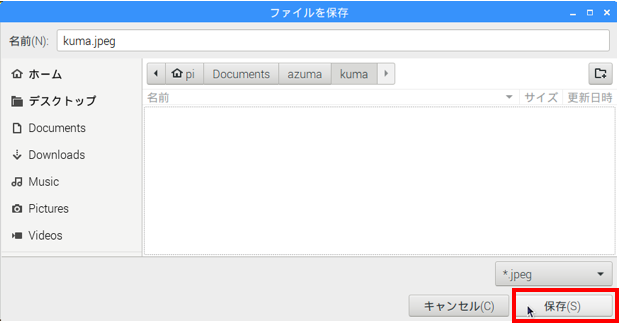
\includegraphics[width=\linewidth]{../../asset/image/textbook-img099.png}
    \flushleft
    8 \ 名前と\ruby{保存}{ほぞん}場所が決まったら右下の\ruby{保存}{ほぞん}をクリック
  \end{minipage}

  \bigskip

  \begin{minipage}{0.4\textwidth}
    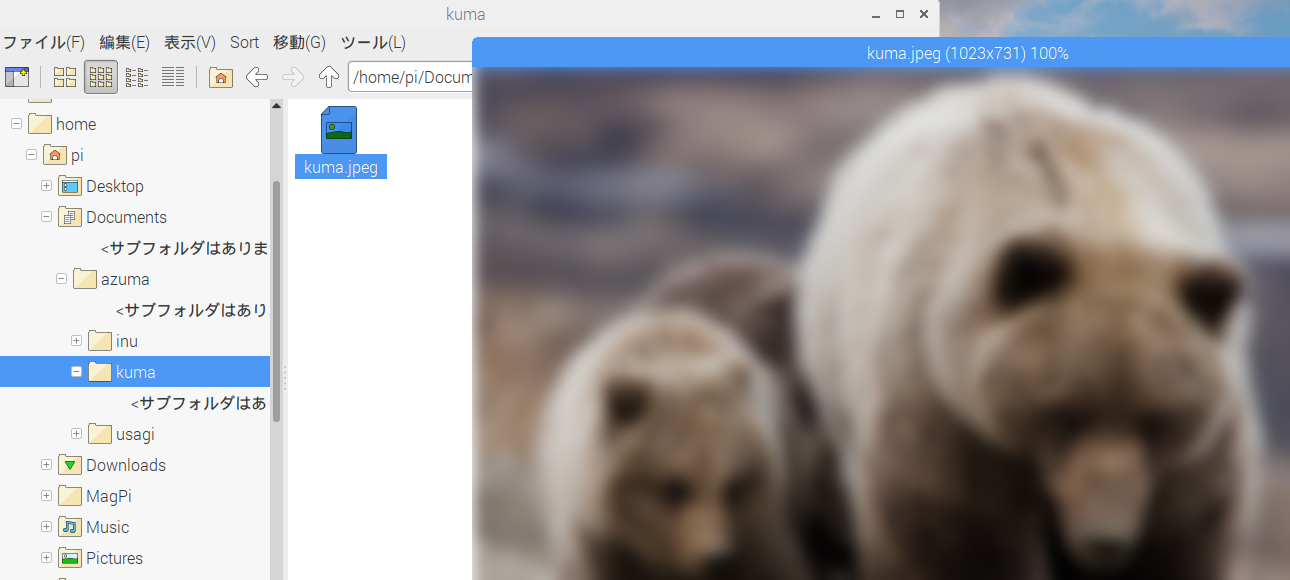
\includegraphics[width=\linewidth]{../../asset/image/textbook-img102.png}
    \flushleft
    9 \ kumaフォルダを開き、\ruby{画像}{がぞう}が\ruby{保存}{ほぞん}されているか、\ruby{確認}{かくにん}しよう
  \end{minipage}
  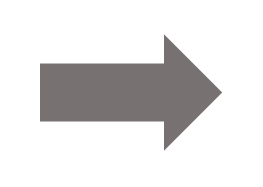
\includegraphics[width=2cm]{../../asset/image/textbook-img073.png}
  \begin{minipage}{0.4\textwidth}
    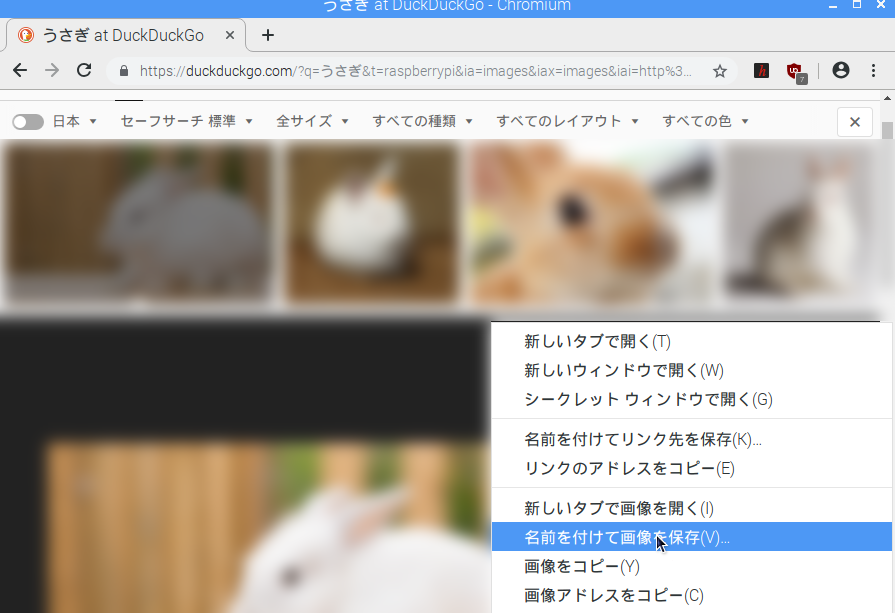
\includegraphics[width=\linewidth]{../../asset/image/textbook-img101.png}
    \flushleft
    10 うさぎで検索し好きな\ruby{画像}{がぞう}を\ruby{保存}{ほぞん}しよう
  \end{minipage}

  \vspace{60mm}

\end{figure}

\bigskip

\clearpage

\begin{figure}[t]
  \textbf{考え方(続き)}

  \begin{minipage}{0.4\textwidth}
    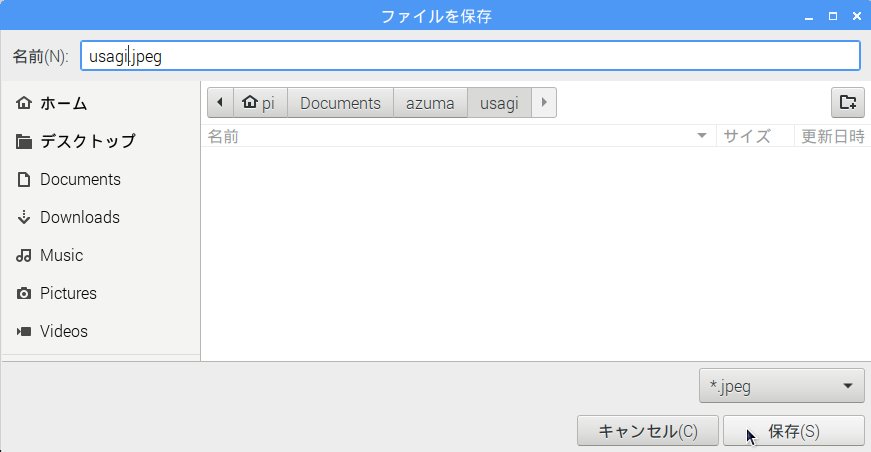
\includegraphics[width=\linewidth]{../../asset/image/textbook-img103.png}
    \flushleft
    11 同じように\ruby{保存}{ほぞん}フォルダと名前を決めて\ruby{保存}{ほぞん}しよう
  \end{minipage}
  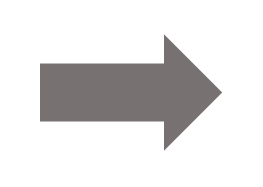
\includegraphics[width=2cm]{../../asset/image/textbook-img073.png}
  \begin{minipage}{0.4\textwidth}
    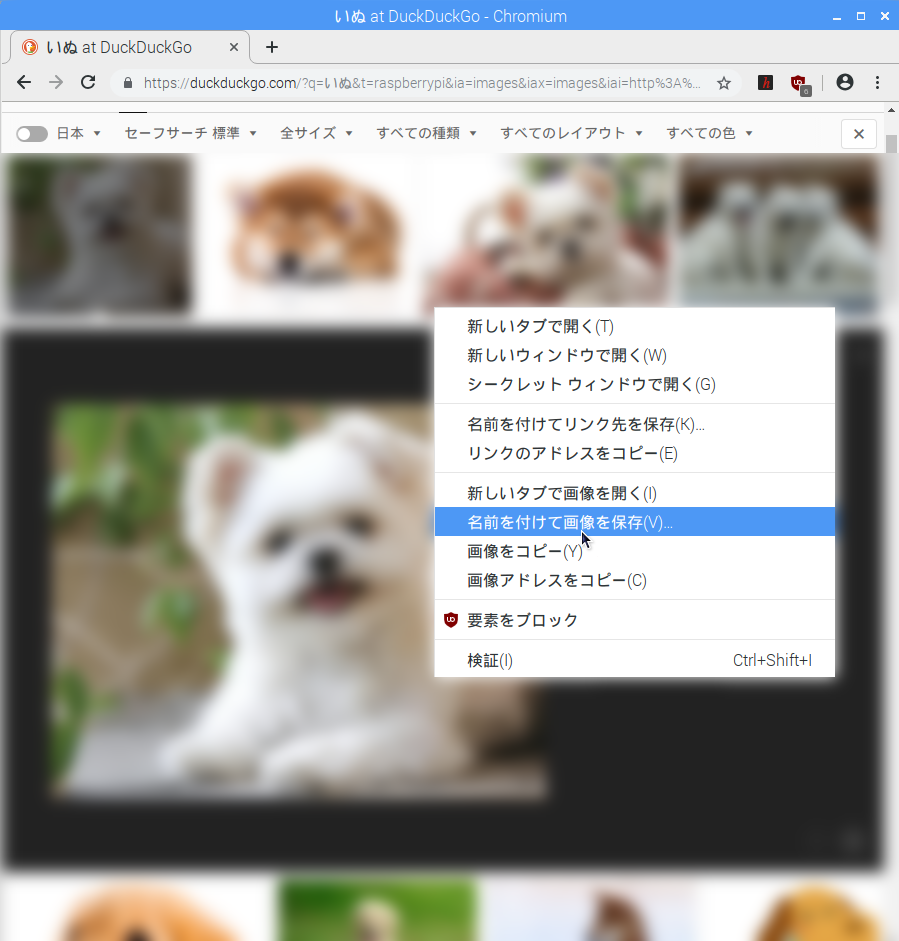
\includegraphics[width=\linewidth]{../../asset/image/textbook-img092.png}
    \flushleft
    12 犬も同様
  \end{minipage}

  \bigskip

  \begin{minipage}{0.4\textwidth}
    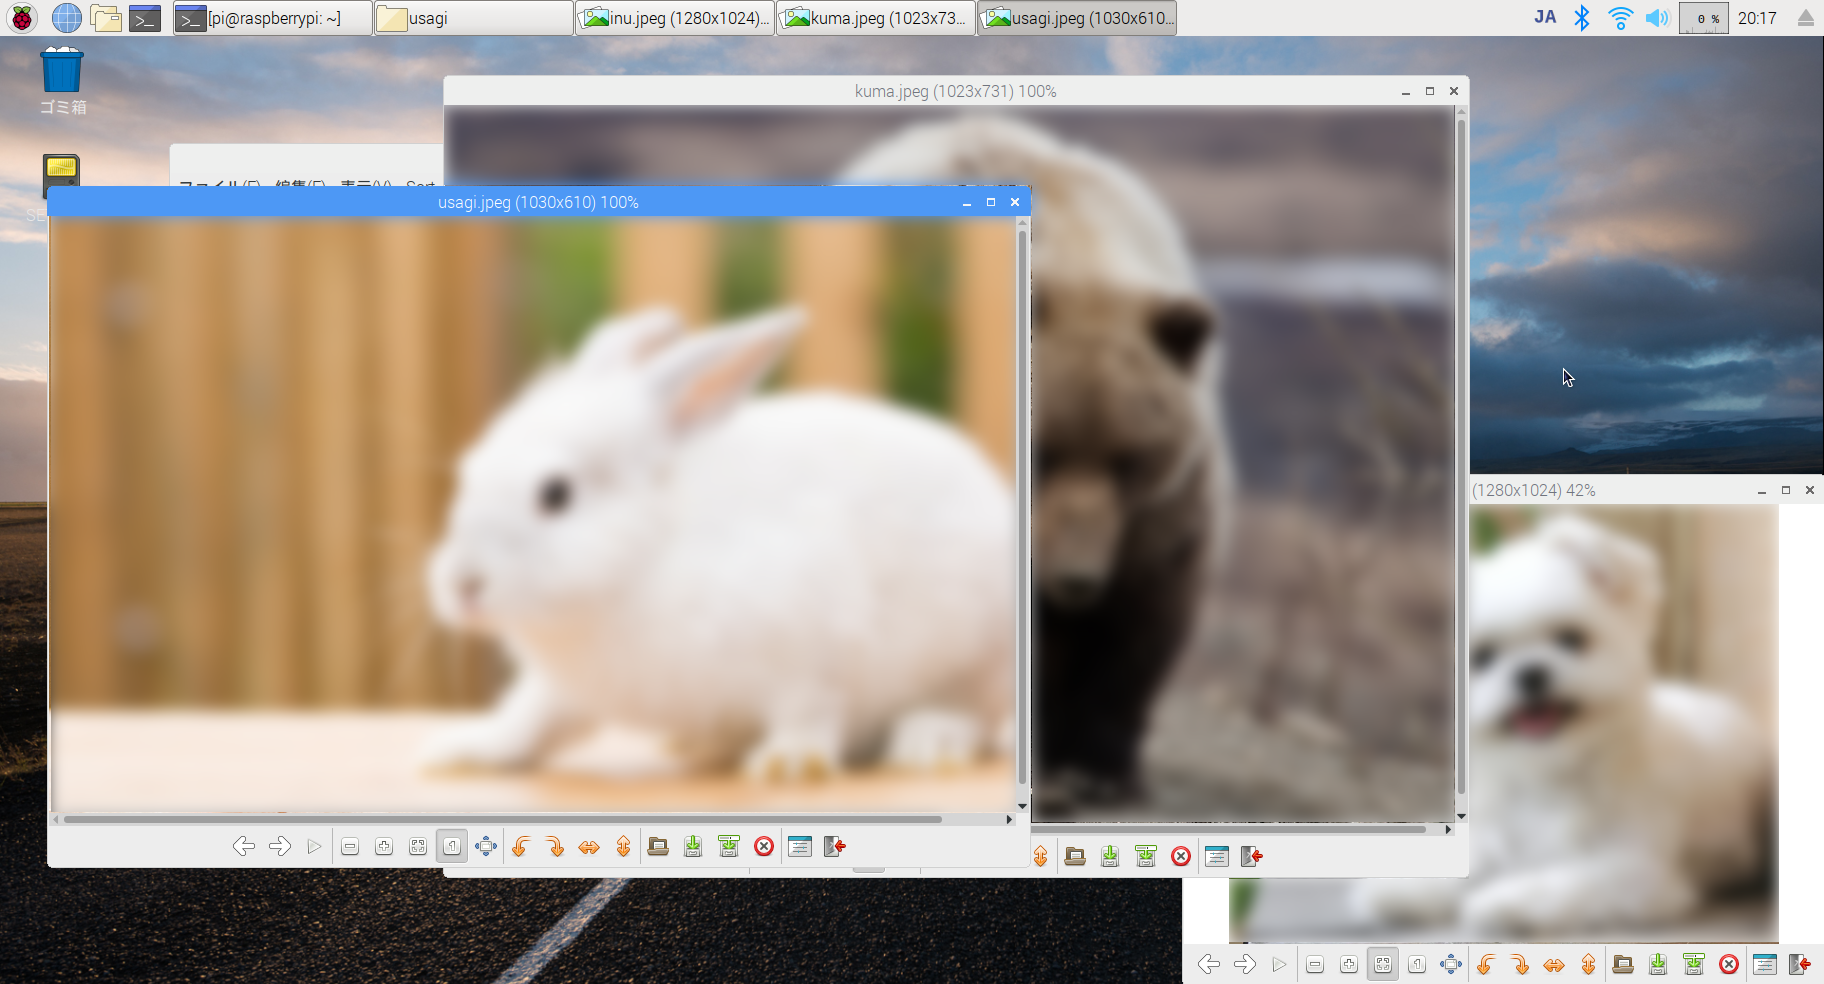
\includegraphics[width=\linewidth]{../../asset/image/textbook-img105.png}
    \flushleft
    13 犬も同様
  \end{minipage}
  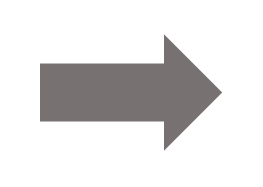
\includegraphics[width=2cm]{../../asset/image/textbook-img073.png}
  \begin{minipage}{0.4\textwidth}
    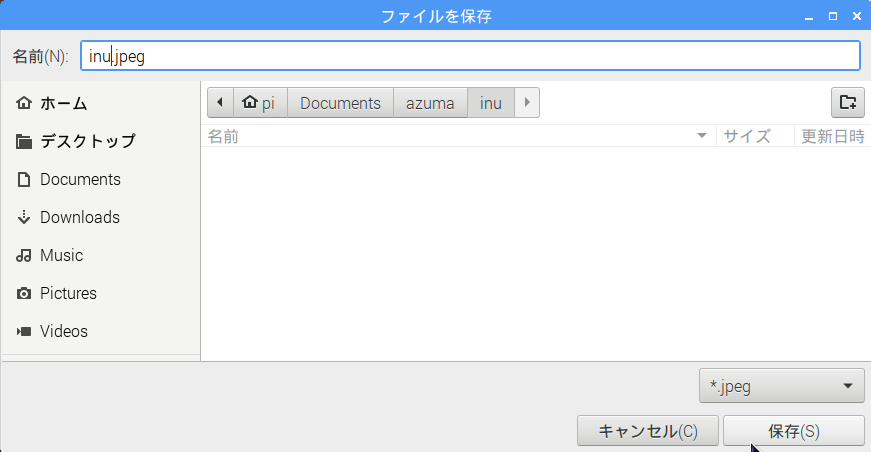
\includegraphics[width=\linewidth]{../../asset/image/textbook-img104.png}
    \flushleft
    14 ruby{保存}{ほぞん}成功
  \end{minipage}

  \centering
\end{figure}

\bigskip

\noindent \textbf{問題 1-13}\\
自分の好きなものの\ruby{画像}{がぞう}を\ruby{保存}{ほぞん}し、自分で作成したフォルダに入れよう。

\clearpage

\begin{figure}
  \subsection{がめんの見た目を自分の好きなものに変えよう}
  
  \subsection{例題 1-14 かべ紙を変えよう}
  \ruby{保存}{ほぞん}した\ruby{画像}{がぞう}をデスクトップのかべ紙にしよう

  \textbf{考え方}
  \bigskip

  \centering
  \begin{minipage}{\textwidth}
    デスクトップのかべ紙は変えることができるよ
    いつも目に入るものだから、自分好みにカスタマイズして気分良く勉強できる\ruby{環境}{かんきょう}にしよう
  \end{minipage}

  \begin{minipage}{0.4\textwidth}
    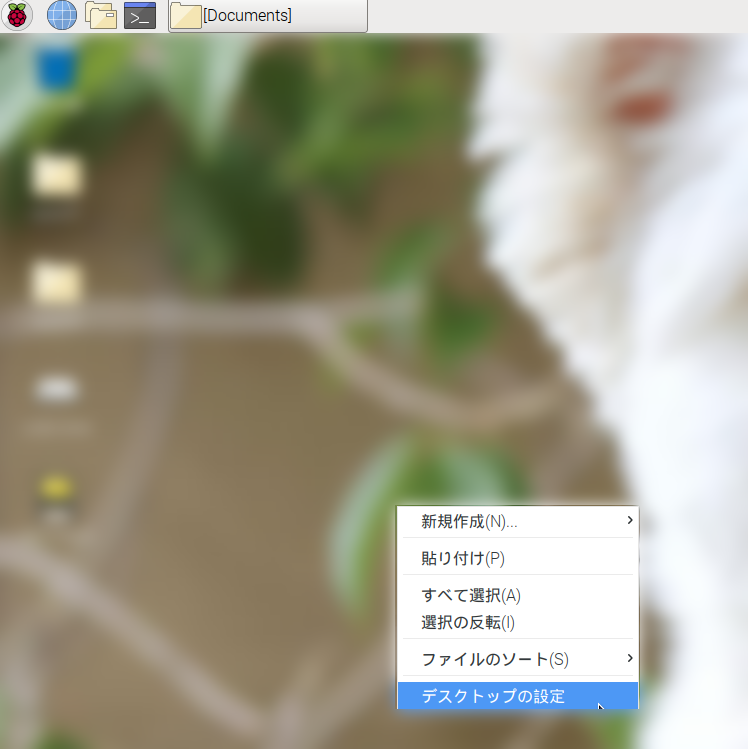
\includegraphics[width=\linewidth]{../../asset/image/textbook-img107.png}
    \flushleft
    1 デスクトップ上で右クリックし、デスクトップの\ruby{設定}{せってい}をクリック
  \end{minipage}
  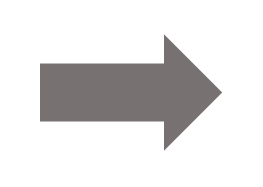
\includegraphics[width=2cm]{../../asset/image/textbook-img073.png}
  \begin{minipage}{0.4\textwidth}
    
\includegraphics[width=0.4\linewidth]{../../asset/image/textbook-img082.png}
    \hfill
    
\includegraphics[width=0.4\linewidth]{../../asset/image/textbook-img106.png}
    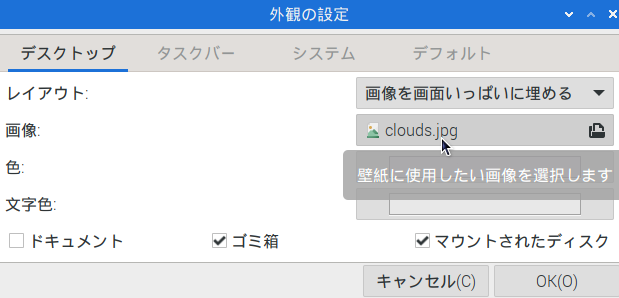
\includegraphics[width=\linewidth]{../../asset/image/textbook-img108.png}
    \flushleft
    2 上の\ruby{画像}{がぞう}のようにクリック
  \end{minipage}

  \begin{minipage}{0.4\textwidth}
    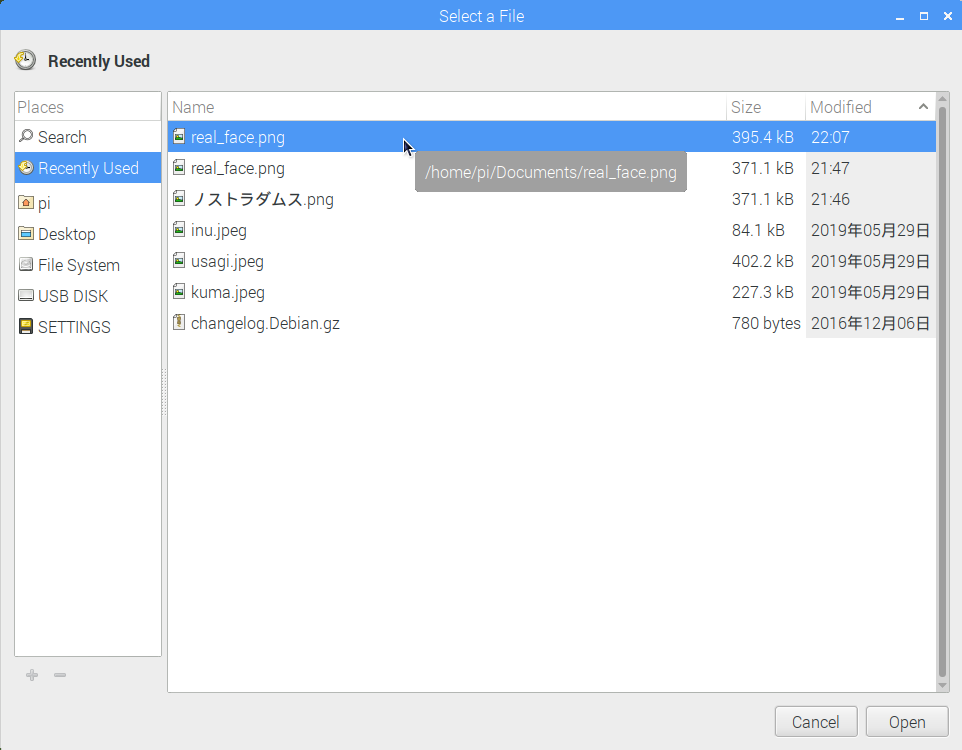
\includegraphics[width=\linewidth]{../../asset/image/textbook-img110.png}
    \flushleft
    3 デスクトップにしたい\ruby{画像}{がぞう}を選ぼう
  \end{minipage}
  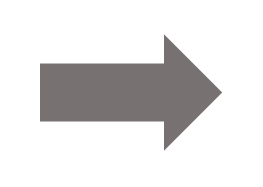
\includegraphics[width=2cm]{../../asset/image/textbook-img073.png}
  \begin{minipage}{0.4\textwidth}
    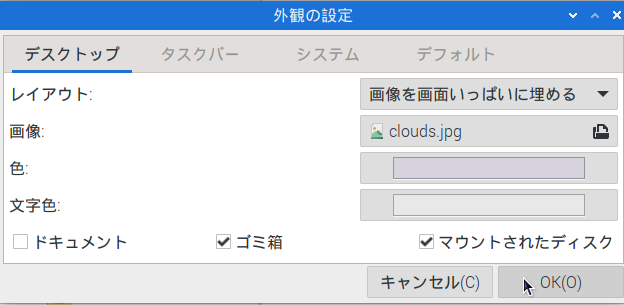
\includegraphics[width=\linewidth]{../../asset/image/textbook-img109.png}
    \flushleft
    4 選び終えたらOKをクリック
  \end{minipage}

  \bigskip


  \flushleft
  \begin{minipage}{0.45\textwidth}
    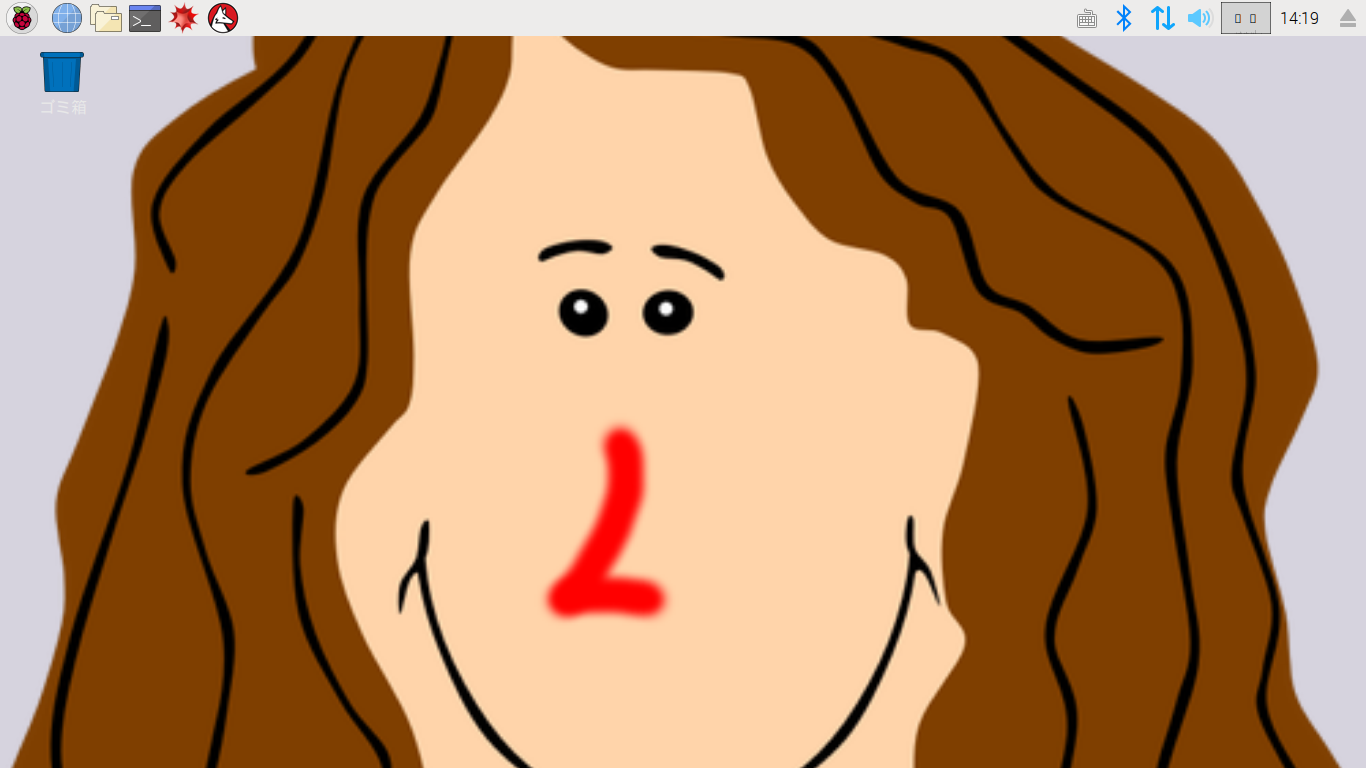
\includegraphics[width=0.85\linewidth]{../../asset/image/textbook-img111.png}\\
    5 デスクトップが変わっているよ
  \end{minipage}

  \bigskip

  \noindent \textbf{問題 1-14}\\
  デスクトップのかべ紙を好きなものに変えてみよう。\ruby{画像}{がぞう}はブラウザでけんさくしてね
\end{figure}

\bigskip

\clearpage
\begin{figure}
  \subsection{例題 1-15 ウィンドウの色を変えてみよう}

  ウィンドウの色を変えてみよう
  
  \textbf{考え方}
  
  \bigskip
  \centering
  \begin{minipage}{\textwidth}
      ウィンドウの色も、デスクトップと同じように変えることができるよ
  \end{minipage}

  \begin{minipage}{0.4\textwidth}
    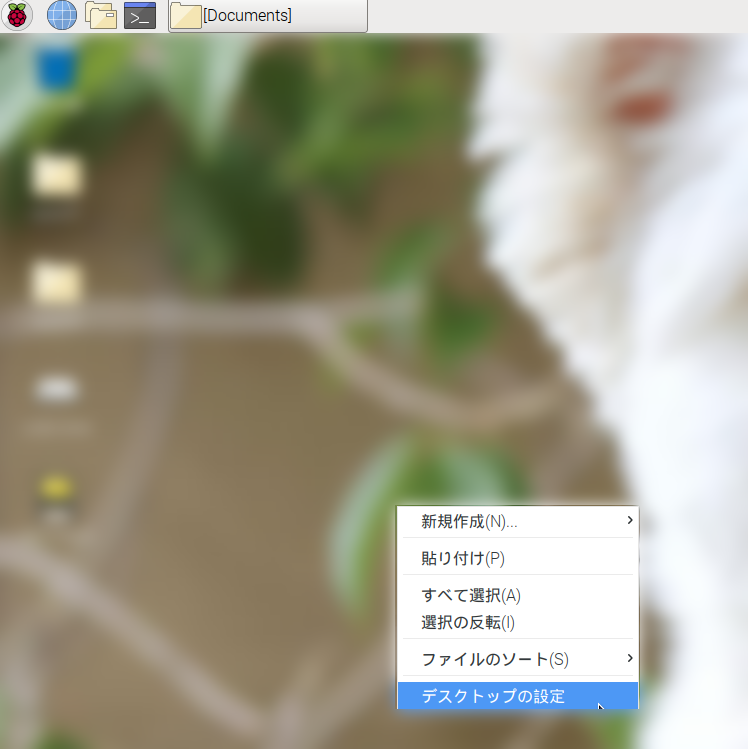
\includegraphics[width=\linewidth]{../../asset/image/textbook-img107.png}
    \flushleft
    1 デスクトップ上で右クリックし、デスクトップの\ruby{設定}{せってい}をクリック
  \end{minipage}
  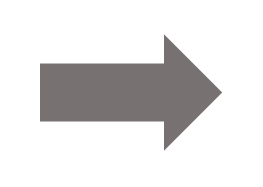
\includegraphics[width=2cm]{../../asset/image/textbook-img073.png}
  \begin{minipage}{0.4\textwidth}
    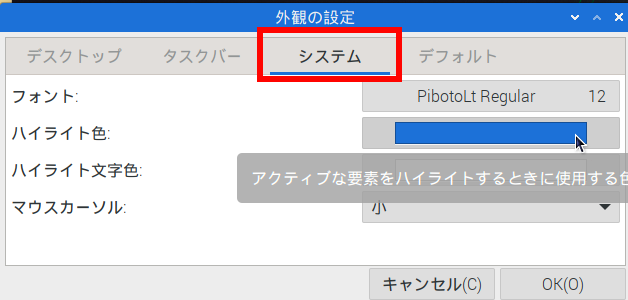
\includegraphics[width=\linewidth]{../../asset/image/textbook-img1001.png}
    \flushleft
    2 上の{画像}{がぞう}の赤く囲われた「システム」をクリックした後、下の「ハイライト色」をクリック
  \end{minipage}

  \begin{minipage}{0.4\textwidth}
    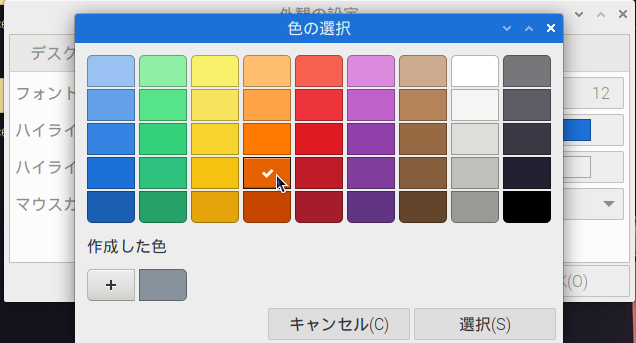
\includegraphics[width=\linewidth]{../../asset/image/textbook-img1002.png}
    \flushleft
    3 すきな色を選ぼう
  \end{minipage}
  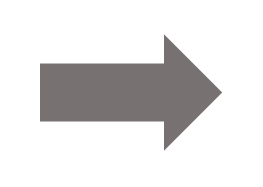
\includegraphics[width=2cm]{../../asset/image/textbook-img073.png}
  \begin{minipage}{0.4\textwidth}
    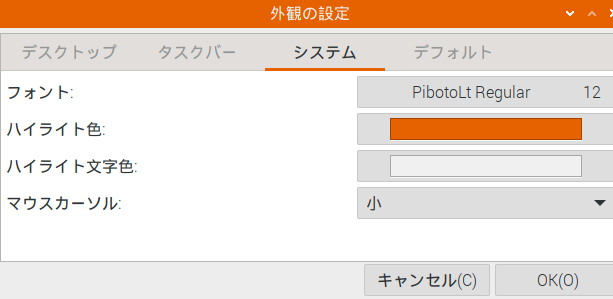
\includegraphics[width=\linewidth]{../../asset/image/textbook-img1003.png}
    \flushleft
    4 選び終えたら、自動的にウィンドウの色が変わっているよ
  \end{minipage}

  \flushleft
  \noindent \textbf{問題 1-15}\\
  UIを好きな色に変えてみよう。

\end{figure}


\bigskip

\clearpage

\end{document}
